
%% main.tex (based on bare_jrnl_compsoc.tex)
%% V1.4b
%% 2015/08/26
%% by Michael Shell
%% See:
%% http://www.michaelshell.org/
%% for current contact information.
%%
%% This is a skeleton file demonstrating the use of IEEEtran.cls
%% (requires IEEEtran.cls version 1.8b or later) with an IEEE
%% Computer Society journal paper.
%%
%% Support sites:
%% http://www.michaelshell.org/tex/ieeetran/
%% http://www.ctan.org/pkg/ieeetran
%% and
%% http://www.ieee.org/

%%*************************************************************************
%% Legal Notice:
%% This code is offered as-is without any warranty either expressed or
%% implied; without even the implied warranty of MERCHANTABILITY or
%% FITNESS FOR A PARTICULAR PURPOSE! 
%% User assumes all risk.
%% In no event shall the IEEE or any contributor to this code be liable for
%% any damages or losses, including, but not limited to, incidental,
%% consequential, or any other damages, resulting from the use or misuse
%% of any information contained here.
%%
%% All comments are the opinions of their respective authors and are not
%% necessarily endorsed by the IEEE.
%%
%% This work is distributed under the LaTeX Project Public License (LPPL)
%% ( http://www.latex-project.org/ ) version 1.3, and may be freely used,
%% distributed and modified. A copy of the LPPL, version 1.3, is included
%% in the base LaTeX documentation of all distributions of LaTeX released
%% 2003/12/01 or later.
%% Retain all contribution notices and credits.
%% ** Modified files should be clearly indicated as such, including  **
%% ** renaming them and changing author support contact information. **
%%*************************************************************************


% *** Authors should verify (and, if needed, correct) their LaTeX system  ***
% *** with the testflow diagnostic prior to trusting their LaTeX platform ***
% *** with production work. The IEEE's font choices and paper sizes can   ***
% *** trigger bugs that do not appear when using other class files.       ***                          ***
% The testflow support page is at:
% http://www.michaelshell.org/tex/testflow/


\documentclass[10pt,journal,compsoc]{IEEEtran}
%
% If IEEEtran.cls has not been installed into the LaTeX system files,
% manually specify the path to it like:
% \documentclass[10pt,journal,compsoc]{../sty/IEEEtran}



\usepackage[T1]{fontenc}
\usepackage{microtype}
\usepackage{graphicx}
\usepackage{listings}
\usepackage{wrapfig}
\usepackage{enumitem}
\usepackage{balance}
\usepackage{float}
\usepackage{url}
\usepackage{tabularx}
\usepackage[table]{xcolor}
\usepackage{booktabs}
\usepackage{subfigure} 
\usepackage{multirow}
\usepackage{mdframed}


% Some very useful LaTeX packages include:
% (uncomment the ones you want to load)


% *** MISC UTILITY PACKAGES ***
%
%\usepackage{ifpdf}
% Heiko Oberdiek's ifpdf.sty is very useful if you need conditional
% compilation based on whether the output is pdf or dvi.
% usage:
% \ifpdf
%   % pdf code
% \else
%   % dvi code
% \fi
% The latest version of ifpdf.sty can be obtained from:
% http://www.ctan.org/pkg/ifpdf
% Also, note that IEEEtran.cls V1.7 and later provides a builtin
% \ifCLASSINFOpdf conditional that works the same way.
% When switching from latex to pdflatex and vice-versa, the compiler may
% have to be run twice to clear warning/error messages.






% *** CITATION PACKAGES ***
%
\ifCLASSOPTIONcompsoc
  % IEEE Computer Society needs nocompress option
  % requires cite.sty v4.0 or later (November 2003)
  \usepackage[nocompress]{cite}
\else
  % normal IEEE
  \usepackage{cite}
\fi
% cite.sty was written by Donald Arseneau
% V1.6 and later of IEEEtran pre-defines the format of the cite.sty package
% \cite{} output to follow that of the IEEE. Loading the cite package will
% result in citation numbers being automatically sorted and properly
% "compressed/ranged". e.g., [1], [9], [2], [7], [5], [6] without using
% cite.sty will become [1], [2], [5]--[7], [9] using cite.sty. cite.sty's
% \cite will automatically add leading space, if needed. Use cite.sty's
% noadjust option (cite.sty V3.8 and later) if you want to turn this off
% such as if a citation ever needs to be enclosed in parenthesis.
% cite.sty is already installed on most LaTeX systems. Be sure and use
% version 5.0 (2009-03-20) and later if using hyperref.sty.
% The latest version can be obtained at:
% http://www.ctan.org/pkg/cite
% The documentation is contained in the cite.sty file itself.
%
% Note that some packages require special options to format as the Computer
% Society requires. In particular, Computer Society  papers do not use
% compressed citation ranges as is done in typical IEEE papers
% (e.g., [1]-[4]). Instead, they list every citation separately in order
% (e.g., [1], [2], [3], [4]). To get the latter we need to load the cite
% package with the nocompress option which is supported by cite.sty v4.0
% and later. Note also the use of a CLASSOPTION conditional provided by
% IEEEtran.cls V1.7 and later.





% *** GRAPHICS RELATED PACKAGES ***
%
\ifCLASSINFOpdf
  % \usepackage[pdftex]{graphicx}
  % declare the path(s) where your graphic files are
  % \graphicspath{{../pdf/}{../jpeg/}}
  % and their extensions so you won't have to specify these with
  % every instance of \includegraphics
  % \DeclareGraphicsExtensions{.pdf,.jpeg,.png}
\else
  % or other class option (dvipsone, dvipdf, if not using dvips). graphicx
  % will default to the driver specified in the system graphics.cfg if no
  % driver is specified.
  % \usepackage[dvips]{graphicx}
  % declare the path(s) where your graphic files are
  % \graphicspath{{../eps/}}
  % and their extensions so you won't have to specify these with
  % every instance of \includegraphics
  % \DeclareGraphicsExtensions{.eps}
\fi
% graphicx was written by David Carlisle and Sebastian Rahtz. It is
% required if you want graphics, photos, etc. graphicx.sty is already
% installed on most LaTeX systems. The latest version and documentation
% can be obtained at: 
% http://www.ctan.org/pkg/graphicx
% Another good source of documentation is "Using Imported Graphics in
% LaTeX2e" by Keith Reckdahl which can be found at:
% http://www.ctan.org/pkg/epslatex
%
% latex, and pdflatex in dvi mode, support graphics in encapsulated
% postscript (.eps) format. pdflatex in pdf mode supports graphics
% in .pdf, .jpeg, .png and .mps (metapost) formats. Users should ensure
% that all non-photo figures use a vector format (.eps, .pdf, .mps) and
% not a bitmapped formats (.jpeg, .png). The IEEE frowns on bitmapped formats
% which can result in "jaggedy"/blurry rendering of lines and letters as
% well as large increases in file sizes.
%
% You can find documentation about the pdfTeX application at:
% http://www.tug.org/applications/pdftex






% *** MATH PACKAGES ***
%
\usepackage{amsmath}
% A popular package from the American Mathematical Society that provides
% many useful and powerful commands for dealing with mathematics.
%
% Note that the amsmath package sets \interdisplaylinepenalty to 10000
% thus preventing page breaks from occurring within multiline equations. Use:
\interdisplaylinepenalty=2500
% after loading amsmath to restore such page breaks as IEEEtran.cls normally
% does. amsmath.sty is already installed on most LaTeX systems. The latest
% version and documentation can be obtained at:
% http://www.ctan.org/pkg/amsmath





% *** SPECIALIZED LIST PACKAGES ***
%
%\usepackage{algorithmic}
% algorithmic.sty was written by Peter Williams and Rogerio Brito.
% This package provides an algorithmic environment fo describing algorithms.
% You can use the algorithmic environment in-text or within a figure
% environment to provide for a floating algorithm. Do NOT use the algorithm
% floating environment provided by algorithm.sty (by the same authors) or
% algorithm2e.sty (by Christophe Fiorio) as the IEEE does not use dedicated
% algorithm float types and packages that provide these will not provide
% correct IEEE style captions. The latest version and documentation of
% algorithmic.sty can be obtained at:
% http://www.ctan.org/pkg/algorithms
% Also of interest may be the (relatively newer and more customizable)
% algorithmicx.sty package by Szasz Janos:
% http://www.ctan.org/pkg/algorithmicx




% *** ALIGNMENT PACKAGES ***
%
%\usepackage{array}
% Frank Mittelbach's and David Carlisle's array.sty patches and improves
% the standard LaTeX2e array and tabular environments to provide better
% appearance and additional user controls. As the default LaTeX2e table
% generation code is lacking to the point of almost being broken with
% respect to the quality of the end results, all users are strongly
% advised to use an enhanced (at the very least that provided by array.sty)
% set of table tools. array.sty is already installed on most systems. The
% latest version and documentation can be obtained at:
% http://www.ctan.org/pkg/array


% IEEEtran contains the IEEEeqnarray family of commands that can be used to
% generate multiline equations as well as matrices, tables, etc., of high
% quality.




% *** SUBFIGURE PACKAGES ***
%\ifCLASSOPTIONcompsoc
%  \usepackage[caption=false,font=footnotesize,labelfont=sf,textfont=sf]{subfig}
%\else
%  \usepackage[caption=false,font=footnotesize]{subfig}
%\fi
% subfig.sty, written by Steven Douglas Cochran, is the modern replacement
% for subfigure.sty, the latter of which is no longer maintained and is
% incompatible with some LaTeX packages including fixltx2e. However,
% subfig.sty requires and automatically loads Axel Sommerfeldt's caption.sty
% which will override IEEEtran.cls' handling of captions and this will result
% in non-IEEE style figure/table captions. To prevent this problem, be sure
% and invoke subfig.sty's "caption=false" package option (available since
% subfig.sty version 1.3, 2005/06/28) as this is will preserve IEEEtran.cls
% handling of captions.
% Note that the Computer Society format requires a sans serif font rather
% than the serif font used in traditional IEEE formatting and thus the need
% to invoke different subfig.sty package options depending on whether
% compsoc mode has been enabled.
%
% The latest version and documentation of subfig.sty can be obtained at:
% http://www.ctan.org/pkg/subfig




% *** FLOAT PACKAGES ***
%
%\usepackage{fixltx2e}
% fixltx2e, the successor to the earlier fix2col.sty, was written by
% Frank Mittelbach and David Carlisle. This package corrects a few problems
% in the LaTeX2e kernel, the most notable of which is that in current
% LaTeX2e releases, the ordering of single and double column floats is not
% guaranteed to be preserved. Thus, an unpatched LaTeX2e can allow a
% single column figure to be placed prior to an earlier double column
% figure.
% Be aware that LaTeX2e kernels dated 2015 and later have fixltx2e.sty's
% corrections already built into the system in which case a warning will
% be issued if an attempt is made to load fixltx2e.sty as it is no longer
% needed.
% The latest version and documentation can be found at:
% http://www.ctan.org/pkg/fixltx2e


%\usepackage{stfloats}
% stfloats.sty was written by Sigitas Tolusis. This package gives LaTeX2e
% the ability to do double column floats at the bottom of the page as well
% as the top. (e.g., "\begin{figure*}[!b]" is not normally possible in
% LaTeX2e). It also provides a command:
%\fnbelowfloat
% to enable the placement of footnotes below bottom floats (the standard
% LaTeX2e kernel puts them above bottom floats). This is an invasive package
% which rewrites many portions of the LaTeX2e float routines. It may not work
% with other packages that modify the LaTeX2e float routines. The latest
% version and documentation can be obtained at:
% http://www.ctan.org/pkg/stfloats
% Do not use the stfloats baselinefloat ability as the IEEE does not allow
% \baselineskip to stretch. Authors submitting work to the IEEE should note
% that the IEEE rarely uses double column equations and that authors should try
% to avoid such use. Do not be tempted to use the cuted.sty or midfloat.sty
% packages (also by Sigitas Tolusis) as the IEEE does not format its papers in
% such ways.
% Do not attempt to use stfloats with fixltx2e as they are incompatible.
% Instead, use Morten Hogholm'a dblfloatfix which combines the features
% of both fixltx2e and stfloats:
%
% \usepackage{dblfloatfix}
% The latest version can be found at:
% http://www.ctan.org/pkg/dblfloatfix




%\ifCLASSOPTIONcaptionsoff
%  \usepackage[nomarkers]{endfloat}
% \let\MYoriglatexcaption\caption
% \renewcommand{\caption}[2][\relax]{\MYoriglatexcaption[#2]{#2}}
%\fi
% endfloat.sty was written by James Darrell McCauley, Jeff Goldberg and 
% Axel Sommerfeldt. This package may be useful when used in conjunction with 
% IEEEtran.cls'  captionsoff option. Some IEEE journals/societies require that
% submissions have lists of figures/tables at the end of the paper and that
% figures/tables without any captions are placed on a page by themselves at
% the end of the document. If needed, the draftcls IEEEtran class option or
% \CLASSINPUTbaselinestretch interface can be used to increase the line
% spacing as well. Be sure and use the nomarkers option of endfloat to
% prevent endfloat from "marking" where the figures would have been placed
% in the text. The two hack lines of code above are a slight modification of
% that suggested by in the endfloat docs (section 8.4.1) to ensure that
% the full captions always appear in the list of figures/tables - even if
% the user used the short optional argument of \caption[]{}.
% IEEE papers do not typically make use of \caption[]'s optional argument,
% so this should not be an issue. A similar trick can be used to disable
% captions of packages such as subfig.sty that lack options to turn off
% the subcaptions:
% For subfig.sty:
% \let\MYorigsubfloat\subfloat
% \renewcommand{\subfloat}[2][\relax]{\MYorigsubfloat[]{#2}}
% However, the above trick will not work if both optional arguments of
% the \subfloat command are used. Furthermore, there needs to be a
% description of each subfigure *somewhere* and endfloat does not add
% subfigure captions to its list of figures. Thus, the best approach is to
% avoid the use of subfigure captions (many IEEE journals avoid them anyway)
% and instead reference/explain all the subfigures within the main caption.
% The latest version of endfloat.sty and its documentation can obtained at:
% http://www.ctan.org/pkg/endfloat
%
% The IEEEtran \ifCLASSOPTIONcaptionsoff conditional can also be used
% later in the document, say, to conditionally put the References on a 
% page by themselves.




% *** PDF, URL AND HYPERLINK PACKAGES ***
%
%\usepackage{url}
% url.sty was written by Donald Arseneau. It provides better support for
% handling and breaking URLs. url.sty is already installed on most LaTeX
% systems. The latest version and documentation can be obtained at:
% http://www.ctan.org/pkg/url
% Basically, \url{my_url_here}.





% *** Do not adjust lengths that control margins, column widths, etc. ***
% *** Do not use packages that alter fonts (such as pslatex).         ***
% There should be no need to do such things with IEEEtran.cls V1.6 and later.
% (Unless specifically asked to do so by the journal or conference you plan
% to submit to, of course. )


% correct bad hyphenation here
\hyphenation{op-tical net-works semi-conduc-tor}


%% our macros and included packages
% \newcommand{\finalVersion} % Uncomment this line to generate a
% production ready pdf

\ifdefined\finalVersion
    \newcommand{\LineComment}[3]{}
\else
    \newcommand{\LineComment}[3]{\textbf{[[#1}{\color{#2} #3}\textbf{]]}}
\fi

\newcommand{\pef}{PEF}
%% please, do not italicize ``i.e.'' and ``e.g.'' - Marcelo
\newcommand{\ie}{i.e.}
\newcommand{\eg}{e.g.}
\newcommand{\etal}{et al.}
\newcommand{\Comment}[1]{}
\newcommand{\CodeIn}[1]{{\small\texttt{#1}}}

\newcommand{\Fix}[1]{\LineComment{}{red}{#1}}
\newcommand{\Jbc}[1]{\LineComment{Jean: }{orange}{#1}}
\newcommand{\Luis}[1]{\LineComment{Luis: }{darkblue}{#1}}
\newcommand{\Mar}[1]{\LineComment{Marcelo: }{darkgreen}{#1}}

%% use this macros
\newcommand{\github}{Github} %% change consistently
\newcommand{\pomf}{\emph{pom.xml}} %% change consistently

%% Evaluation macros

%% SUBJECTS
\newcommand{\SubjectsGithub}{813}
\newcommand{\SubjectsGithubNotMaven}{\Fix{48}}
\newcommand{\SubjectsGithubNotTestable}{\Fix{132}}
\newcommand{\SubjectsGithubFlaky}{\Fix{16}}
\newcommand{\numSubjs}{390}
\newcommand{\numSubjsShort}{307}
\newcommand{\numSubjsMed}{49}
\newcommand{\numSubjsLong}{34}

%% CONFIGURATION MODES
\newcommand{\Seq}{C0}
\newcommand{\SeqClassParMeth}{C1}
\newcommand{\ParClassSeqMeth}{C2}
\newcommand{\ParClassParMeth}{C3}
\newcommand{\Fork}{F}
\newcommand{\ForkSeq}{\Fork{}\Seq{}}
\newcommand{\ForkParMeth}{\Fork{}\SeqClassParMeth{}}

%% RQ1
\newcommand{\medg}{medium}
\newcommand{\longg}{long}
\newcommand{\shortg}{short}

\newcommand{\numSubjsPass}{250}
\newcommand{\numSubjsFail}{140}

\newcommand{\numMed}{\Fix{49}}
\newcommand{\numLong}{\Fix{34}}
\newcommand{\numMedLong}{83}
\newcommand{\percentMedLongRunning}{21\%}
\newcommand{\percentLongRunning}{8.7\%}

%% RQ3&RQ4
\newcommand{\avgSpeedup}{4.4}
\newcommand{\pomMedLong}{67}
\newcommand{\numPomMed}{38}
\newcommand{\numPomLong}{29}
\newcommand{\numPomMatched}{\pomMedLong{}}
\newcommand{\percentParallel}{13.3\%}
\newcommand{\percentParallelUpdated}{18.1\%}
\newcommand{\numNonParallel}{74}
%% \newcommand{\numPomMatchedValid}{\Fix{103}}
\newcommand{\numProjectsPar}{nine}
\newcommand{\percentShortSequential}{\Fix{96.7\%}}

\newcommand{\averageMedLongRunning}{8m36s}
\newcommand{\percentParallelForLongRunning}{\Fix{80\%}}

%% RQ5
\newcommand{\emailsSent}{297}
\newcommand{\emailsFalseAnswers}{three}
\newcommand{\emailsTrueAnswers}{32}
\newcommand{\emailsProjectsAnswered}{36}
\newcommand{\percEmailsProjectsAnswered}{61.29\%}
\newcommand{\emailsAnswered}{38}
\newcommand{\percEmailsAnswered}{12.8\%}
\newcommand{\discartedProjects}{10}
\newcommand{\emailsProjects}{62}

%% RQ5 Survey answers
\newcommand{\emailsCI}{12} % 8 + distributed
\newcommand{\emailsLocal}{6}
\newcommand{\emailsDistributed}{4}
\newcommand{\emailsNotDescribed}{14}

\newcommand{\emailsSequential}{30}
\newcommand{\emailsParallel}{6}

\newcommand{\emailsA}{8.33\%} %3
\newcommand{\emailsB}{33.33\%} %12
\newcommand{\emailsC}{22.22\%} %8
\newcommand{\emailsD}{16.67\%} %6
\newcommand{\emailsNA}{19.45\%} %7

\newcommand{\webpage}{\url{https://doubleblind.000webhostapp.com/}}



\begin{document}
%
% paper title
% Titles are generally capitalized except for words such as a, an, and, as,
% at, but, by, for, in, nor, of, on, or, the, to and up, which are usually
% not capitalized unless they are the first or last word of the title.
% Linebreaks \\ can be used within to get better formatting as desired.
% Do not put math or special symbols in the title.
\title{Test Suite Parallelization in Open-Source Projects:\\ A Study on Its Usage and Impact}
%
%
% author names and IEEE memberships
% note positions of commas and nonbreaking spaces ( ~ ) LaTeX will not break
% a structure at a ~ so this keeps an author's name from being broken across
% two lines.
% use \thanks{} to gain access to the first footnote area
% a separate \thanks must be used for each paragraph as LaTeX2e's \thanks
% was not built to handle multiple paragraphs
%
%
%\IEEEcompsocitemizethanks is a special \thanks that produces the bulleted
% lists the Computer Society journals use for "first footnote" author
% affiliations. Use \IEEEcompsocthanksitem which works much like \item
% for each affiliation group. When not in compsoc mode,
% \IEEEcompsocitemizethanks becomes like \thanks and
% \IEEEcompsocthanksitem becomes a line break with idention. This
% facilitates dual compilation, although admittedly the differences in the
% desired content of \author between the different types of papers makes a
% one-size-fits-all approach a daunting prospect. For instance, compsoc 
% journal papers have the author affiliations above the "Manuscript
% received ..."  text while in non-compsoc journals this is reversed. Sigh.

\author{Michael~Shell,~\IEEEmembership{Member,~IEEE,}
        John~Doe,~\IEEEmembership{Fellow,~OSA,}
        and~Jane~Doe,~\IEEEmembership{Life~Fellow,~IEEE}% <-this % stops a space
\IEEEcompsocitemizethanks{\IEEEcompsocthanksitem M. Shell was with the Department
of Electrical and Computer Engineering, Georgia Institute of Technology, Atlanta,
GA, 30332.\protect\\
% note need leading \protect in front of \\ to get a newline within \thanks as
% \\ is fragile and will error, could use \hfil\break instead.
E-mail: see http://www.michaelshell.org/contact.html
\IEEEcompsocthanksitem J. Doe and J. Doe are with Anonymous University.}% <-this % stops an unwanted space
\thanks{Manuscript received April 19, 2005; revised August 26, 2015.}}

% note the % following the last \IEEEmembership and also \thanks - 
% these prevent an unwanted space from occurring between the last author name
% and the end of the author line. i.e., if you had this:
% 
% \author{....lastname \thanks{...} \thanks{...} }
%                     ^------------^------------^----Do not want these spaces!
%
% a space would be appended to the last name and could cause every name on that
% line to be shifted left slightly. This is one of those "LaTeX things". For
% instance, "\textbf{A} \textbf{B}" will typeset as "A B" not "AB". To get
% "AB" then you have to do: "\textbf{A}\textbf{B}"
% \thanks is no different in this regard, so shield the last } of each \thanks
% that ends a line with a % and do not let a space in before the next \thanks.
% Spaces after \IEEEmembership other than the last one are OK (and needed) as
% you are supposed to have spaces between the names. For what it is worth,
% this is a minor point as most people would not even notice if the said evil
% space somehow managed to creep in.



% The paper headers
\markboth{Journal of \LaTeX\ Class Files,~Vol.~14, No.~8, August~2015}%
{Shell \MakeLowercase{\textit{et al.}}: Bare Demo of IEEEtran.cls for Computer Society Journals}
% The only time the second header will appear is for the odd numbered pages
% after the title page when using the twoside option.
% 
% *** Note that you probably will NOT want to include the author's ***
% *** name in the headers of peer review papers.                   ***
% You can use \ifCLASSOPTIONpeerreview for conditional compilation here if
% you desire.



% The publisher's ID mark at the bottom of the page is less important with
% Computer Society journal papers as those publications place the marks
% outside of the main text columns and, therefore, unlike regular IEEE
% journals, the available text space is not reduced by their presence.
% If you want to put a publisher's ID mark on the page you can do it like
% this:
%\IEEEpubid{0000--0000/00\$00.00~\copyright~2015 IEEE}
% or like this to get the Computer Society new two part style.
%\IEEEpubid{\makebox[\columnwidth]{\hfill 0000--0000/00/\$00.00~\copyright~2015 IEEE}%
%\hspace{\columnsep}\makebox[\columnwidth]{Published by the IEEE Computer Society\hfill}}
% Remember, if you use this you must call \IEEEpubidadjcol in the second
% column for its text to clear the IEEEpubid mark (Computer Society jorunal
% papers don't need this extra clearance.)



% use for special paper notices
%\IEEEspecialpapernotice{(Invited Paper)}



% for Computer Society papers, we must declare the abstract and index terms
% PRIOR to the title within the \IEEEtitleabstractindextext IEEEtran
% command as these need to go into the title area created by \maketitle.
% As a general rule, do not put math, special symbols or citations
% in the abstract or keywords.
\IEEEtitleabstractindextext{%
\begin{abstract}
Dealing with high testing costs remains an important problem in
Software Engineering.  Test suite parallelization is an important
approach to address this problem.  This paper reports our findings on
the usage and impact of test suite parallelization in open-source
projects.\Comment{ This study brings to light the benefits and burdens
  of that approach.} It provides recommendations to practitioners and
tool developers to speed up test execution.

Considering a set of \numSubjs{} popular Java projects we analyzed, we
found that \percentMedLongRunning{} of the projects contain costly
test suites but parallelization features still seem underutilized in
practice~---~only \percentParallelUpdated{} of costly projects use
parallelization.  The main reported reason for adoption resistance was
the concern to deal with concurrency issues.  Results suggest that, on
average, developers prefer high predictability than high performance
in running tests.
\end{abstract}

% Note that keywords are not normally used for peerreview papers.
\begin{IEEEkeywords}
Computer Society, IEEE, IEEEtran, journal, \LaTeX, paper, template.
\end{IEEEkeywords}}


% make the title area
\maketitle


% To allow for easy dual compilation without having to reenter the
% abstract/keywords data, the \IEEEtitleabstractindextext text will
% not be used in maketitle, but will appear (i.e., to be "transported")
% here as \IEEEdisplaynontitleabstractindextext when the compsoc 
% or transmag modes are not selected <OR> if conference mode is selected 
% - because all conference papers position the abstract like regular
% papers do.
\IEEEdisplaynontitleabstractindextext
% \IEEEdisplaynontitleabstractindextext has no effect when using
% compsoc or transmag under a non-conference mode.



% For peer review papers, you can put extra information on the cover
% page as needed:
% \ifCLASSOPTIONpeerreview
% \begin{center} \bfseries EDICS Category: 3-BBND \end{center}
% \fi
%
% For peerreview papers, this IEEEtran command inserts a page break and
% creates the second title. It will be ignored for other modes.
\IEEEpeerreviewmaketitle


% An example of a floating figure using the graphicx package.
% Note that \label must occur AFTER (or within) \caption.
% For figures, \caption should occur after the \includegraphics.
% Note that IEEEtran v1.7 and later has special internal code that
% is designed to preserve the operation of \label within \caption
% even when the captionsoff option is in effect. However, because
% of issues like this, it may be the safest practice to put all your
% \label just after \caption rather than within \caption{}.
%
% Reminder: the "draftcls" or "draftclsnofoot", not "draft", class
% option should be used if it is desired that the figures are to be
% displayed while in draft mode.
%
%\begin{figure}[!t]
%\centering
%\includegraphics[width=2.5in]{myfigure}
% where an .eps filename suffix will be assumed under latex, 
% and a .pdf suffix will be assumed for pdflatex; or what has been declared
% via \DeclareGraphicsExtensions.
%\caption{Simulation results for the network.}
%\label{fig_sim}
%\end{figure}

% Note that the IEEE typically puts floats only at the top, even when this
% results in a large percentage of a column being occupied by floats.
% However, the Computer Society has been known to put floats at the bottom.


% An example of a double column floating figure using two subfigures.
% (The subfig.sty package must be loaded for this to work.)
% The subfigure \label commands are set within each subfloat command,
% and the \label for the overall figure must come after \caption.
% \hfil is used as a separator to get equal spacing.
% Watch out that the combined width of all the subfigures on a 
% line do not exceed the text width or a line break will occur.
%
%\begin{figure*}[!t]
%\centering
%\subfloat[Case I]{\includegraphics[width=2.5in]{box}%
%\label{fig_first_case}}
%\hfil
%\subfloat[Case II]{\includegraphics[width=2.5in]{box}%
%\label{fig_second_case}}
%\caption{Simulation results for the network.}
%\label{fig_sim}
%\end{figure*}
%
% Note that often IEEE papers with subfigures do not employ subfigure
% captions (using the optional argument to \subfloat[]), but instead will
% reference/describe all of them (a), (b), etc., within the main caption.
% Be aware that for subfig.sty to generate the (a), (b), etc., subfigure
% labels, the optional argument to \subfloat must be present. If a
% subcaption is not desired, just leave its contents blank,
% e.g., \subfloat[].


% An example of a floating table. Note that, for IEEE style tables, the
% \caption command should come BEFORE the table and, given that table
% captions serve much like titles, are usually capitalized except for words
% such as a, an, and, as, at, but, by, for, in, nor, of, on, or, the, to
% and up, which are usually not capitalized unless they are the first or
% last word of the caption. Table text will default to \footnotesize as
% the IEEE normally uses this smaller font for tables.
% The \label must come after \caption as always.
%
%\begin{table}[!t]
%% increase table row spacing, adjust to taste
%\renewcommand{\arraystretch}{1.3}
% if using array.sty, it might be a good idea to tweak the value of
% \extrarowheight as needed to properly center the text within the cells
%\caption{An Example of a Table}
%\label{table_example}
%\centering
%% Some packages, such as MDW tools, offer better commands for making tables
%% than the plain LaTeX2e tabular which is used here.
%\begin{tabular}{|c||c|}
%\hline
%One & Two\\
%\hline
%Three & Four\\
%\hline
%\end{tabular}
%\end{table}


% Note that the IEEE does not put floats in the very first column
% - or typically anywhere on the first page for that matter. Also,
% in-text middle ("here") positioning is typically not used, but it
% is allowed and encouraged for Computer Society conferences (but
% not Computer Society journals). Most IEEE journals/conferences use
% top floats exclusively. 
% Note that, LaTeX2e, unlike IEEE journals/conferences, places
% footnotes above bottom floats. This can be corrected via the
% \fnbelowfloat command of the stfloats package.

\Jbc{Review float and text formatting on the whole document.}

\section{Introduction}

Optimizing regression testing is important.  As software evolves the
size of test sets increases, potentially leading to disruption in the
development process caused by late reports of test failures.  This
problem manifests more dramatically at large IT companies
(e.g.,\Comment{ Groupon~\Fix{cite},} Google~\Fix{cite} and
Microsoft~\Fix{cite}) where the size of test sets often exceeds the
size of the code base.  Several approaches have been proposed to
optimize regression testing.  Research has focused mostly on test
selection~\Fix{cite}, test reduction~\Fix{cite}, and test
prioritization~\Fix{cite}.  Although these approaches can also be
applied in industrial settings, the focus in industry has been
mostly in parallelizing execution of tests using server
farms,\Fix{@Jean: Is
this an assumption? Is there any evidence?} where worker machines
from the farm are assigned to execute distinct subsets of the original
test suite.

Given the proliferation of multicore machines it is not surprising
that popular build systems and testing frameworks provide today
support for parallel test execution with the goal of running tests
more efficiently~\cite{junit-org,testng,nunit,maven-surefire-plugin}.
The lower-level parallelism enabled through build systems and testing
frameworks is an important complement to the higher-level parallelism
enabled through server farms.  These solutions enable the use of
commodity hardware to maximize CPU usage\footnote{In the case of the
  Java language, for example, it is possible to explore parallelism
  across and within JVMs.}.  For the scenario of large IT
organizations, lower-level parallelization schemes could leverage the
computing power of server nodes in addition to the aggregate
processing power of the farm.  Lower-level parallelism fits
particularly well smaller organizations (/projects) with relatively
high testing costs but lower budgets.  Unfortunately, these solutions
can't be used out-of-the-box: unrestricted parallel execution of tests
can produce non-deterministic results as developers typically do not
provision protection to concurrent accesses originated from arbitrary
program points (\ie{}, tests).  We refer to this problem as Parallel
Execution Flakiness (\pef{}).

To illustrate the importance of parallel test execution and the
problem of \pef{} let's consider the case of the ``core'' module from
the Apache Camel project~\cite{apache-camel-web}.  This module
contains 5,679 test cases, declared in 2,356 test classes.  We ran
those tests in a machine with 16GB of memory and 8 virtual CPUs (4
cores with 2 native threads each).  Sequential test execution takes
24m50s to run this test set.  Execution of the same test set takes
2m28s when we configured parallel execution to fork a JVM per CPU and
execute test classes, uniquely allocated to that JVM, sequentially but
running test methods from each class in separate threads.  Note that
this is an order of magnitude speedup (10.07x)\Fix{Need to understand
  why this is 10x as opposed to something closer to 7x - I didn't get
  your concern here}.
Unfortunately, due to \pef{}, $\sim$2\% (114 of 5,679) of the tests
fail when executed in parallel.  It is important to notice that the
ratio of failures varies with the project as it depends on factors
such as length of test cases and amount of shared state across tests.

\pef{} is an important obstacle to enable parallel test execution.
Conceptually, higher parallelization can result in higher chances of
concurrency-related problems.  It is important to execute tests
efficiently without sacrificing reliability
\Fix{gap between pars?? What gap?}

This paper reports an empirical study to evaluate the impact of
parallelization options on test execution speedup and \pef{}. Based on
these results, we proposed different low-cost synchronization
strategies to avoid \pef{}.

%%  LocalWords:  parallelization multicore JUnit TestNG NUnit XXm YYm
%%  LocalWords:  Groupon parallelizing multi JVMs CPUs JVM

\section{Parallel Execution of Test Suites}
\label{sec:modes}

Figure~\ref{fig:levels} illustrates different levels where
parallelism in test execution can be obtained.
The highest level indicates
parallelism obtained through different machines on the
network.  For instance, using virtual machines from a cloud service to
\begin{wrapfigure}{r}{0.13\textwidth}  
  \vspace{-2mm}
  \centering
  %  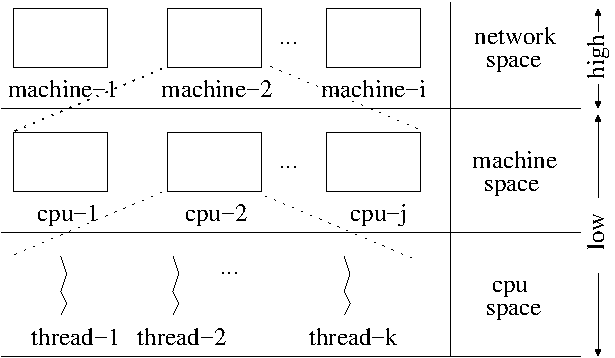
\includegraphics[width=0.35\textwidth]{figs/parallel-levels.pdf}    
  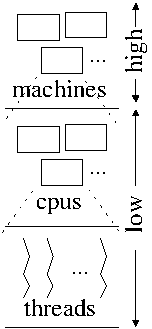
\includegraphics[width=2cm]{figs/parallel-levels-short.pdf}  
  \caption{\label{fig:levels}Levels of parallelism.}
  \vspace{-2mm}
\end{wrapfigure}
distribute test execution.  The lowest levels denote parallelism
obtained within a single machine.  These levels are complementary:
the lowest levels leverage the computing power of server
nodes whereas the highest level leverages the aggregate processing
power of a network of machines.
This paper focuses on low-level parallelism, where computation can be
offloaded at different CPUs within a machine and at different threads
within each CPU.  This form of parallelism is enabled through build
systems (spawning processes in different CPUs) and testing frameworks
(spawning threads in one given CPU).  It is important to note that a variety
of testing frameworks provide today support for parallel test
execution (e.g., JUnit~\cite{junit-org}, TestNG~\cite{testng}, and
NUnit~\cite{nunit}) as to benefit from the available power of popular multi-core processors.
In the following, we elaborate relevant features of testing frameworks
and build systems for parallelization.  We focused on Java, Maven, and JUnit but the
discussion can be generalized to other language and tools.

\subsection{Testing Frameworks}
\label{sec:frameworks}

The list below shows the choices to control parallelism within one
Java Virtual Machine (JVM).  These options are offered by the testing
framework (\eg{}, JUnit).

\begin{itemize}
\item
    \textbf{Sequential (\Seq).}~No parallelism is involved.
\item
    \textbf{Sequential classes; parallel methods
      (\SeqClassParMeth).}~This configuration corresponds to running
    test classes sequentially, but running test methods from those
    classes concurrently.
\item
    \textbf{Parallel classes; sequential methods
      (\ParClassSeqMeth{}).}~This configuration corresponds to running
    test classes concurrently, but running test methods sequentially.
\item
    \textbf{Parallel classes; Parallel methods
      (\ParClassParMeth).}~This configuration runs test classes and
    methods concurrently.\Comment{corresponds to the
    combination of \SeqClassParMeth{} and \ParClassSeqMeth{}.  }
\end{itemize}

Notice that an important aspect in deciding which configuration to use (or in
designing new test suites) is the possibility of race conditions on shared data
during execution.  Data sharing can occur, for example, through state that is
reachable from statically-declared variables in the program or through variables
declared within the scope of the test class or even through resources available
on the file system and the network~\cite{luo-etal-fse2014}.  Considering data
race avoidance, configuration \SeqClassParMeth{} is preferable over
\ParClassSeqMeth{} when it is clear that test methods in a class do not
manipulate shared state, which can be challenging to
determine~\cite{bell-etal-esecfse2015}.  Similarly, \ParClassSeqMeth{} is
preferable over \SeqClassParMeth{} when it is clear that several test methods in
a class perform operations involving shared data.  Configuration
\ParClassParMeth{} does not restrict scheduling orderings.  Consequently, it is
more likely to manifest data races during execution. Note that speedups depend
on several factors, including the test suite size and distribution of test
methods per class.

\subsection{Build Systems}
\label{sec:builder}

%% The build system can spawn multiple JVMs, each running on its own OS
%% process on a given CPU and handling a partition of the test set.
Forking OS processes to run test jobs is the basic mechanism of build
systems to obtain parallelism at the machine space (see
Figure~\ref{fig:levels}).  For Java-based build systems, such as Maven
and Ant, this amounts to spawning one JVM, on a given CPU, to handle a
test job and aggregating results when jobs finish.  The list below
shows the choices to control parallelism through the build system
(\eg{}, Maven).

\begin{itemize}
\item
  \textbf{Forked JVMs with sequential methods (\ForkSeq).}~The build
  system spawns multiple JVMs with this configuration, assigning a
  partition of the set of test classes to each JVM.  Test classes and methods
  run sequentially within each JVM.
\item
  \textbf{Forked JVMs with parallel methods (\ForkParMeth).}~With
  this configuration, the build system forks multiple JVMs, as
  \ForkSeq{} does, but it runs test methods concurrently, as
  \SeqClassParMeth{} does.
\end{itemize}

%% In the configuration \ForkSeq{}, each spawned
%% process runs a different test class at time and the builder merges the
%% results from each execution. In the configuration \ForkParMeth{}, the
%% build system forwards settings to the underlying testing framework to
%% enable parallel execution within each process in addition to running
%% test classes on different processes.

Note from the listing that forking can only be combined with
configuration \SeqClassParMeth{} (see Section~\ref{sec:frameworks}) as
Maven made the design choice to only accept one test class at a time
per forked process.  Maven offers an option to reuse JVMs that can be
used to attenuate the potentially high cost of spawning new JVM
processes on every test class (if reuse is enabled) and also to
achieve test isolation (if reuse is disabled).

%% \Mar{$\leftarrow$Are you sure about this?
%%   It seems silly.  Maybe, the rationale is to ``keep design
%%   simple''.}\Jbc{I'm sure. in addition to keep design simple, I feel
%%   like this was initially conceived to run tests in isolation}
%% \Mar{$\leftarrow$confirma?  se sim, pode mostrar isto na
%%   configuracao abaixo?}\Jbc{added...}
%%We are unaware of other build system capable of running multiple
%%classes at time within a forked process.
%%  to
%% define tasks related to the project building and these tasks are
%% performed several plugins.This file
%% contains defintions of tasks, which are implemented by a collection of
%% plugins.
%% \Jbc{falar do surefire e explicar a
%% configuracao ilustrada - Surefire levanta uma JVM por core e cria uma
%% pool de 5 threads em cada JVM para executar testes em paralelo.}
\begin{figure}[h!]
\centering
\scriptsize
\lstset{
  escapeinside={@}{@},
  numbers=none,xleftmargin=1em,frame=none,framexleftmargin=0.5em,
  basicstyle=\ttfamily\scriptsize, boxpos=c, numberstyle=\tiny,
  morekeywords={parallel, threadCount, perCoreThreadCount,
  forkCount, reuseForks},
  deletekeywords={true}
}
\vspace{-4ex}
\begin{lstlisting}
<plugin>
    <groupId>org.apache.maven.plugins</groupId>
    <artifactId>maven-surefire-plugin</artifactId>
    <configuration>
        <forkCount>1C</forkCount>
        <reuseForks>true</reuseForks>
        <parallel>methods</parallel>
        <threadCount>5</threadCount>
    </configuration>
</plugin>
\end{lstlisting}
  \vspace{-4ex}
  \caption{\label{fig:surefire} Configuration \ForkParMeth{} on
    Maven.}
\end{figure}


\subsubsection*{Example}~Figure~\ref{fig:surefire} shows a
fragment of a Maven configuration file, known as \pomf{}, highlighting
options to run tests using the parallel execution mode \ForkParMeth{}.
Maven implements this feature through its Surefire JUnit test
plugin~\cite{maven-surefire-plugin}.  With this configuration, Maven
forks one JVM per core (\CodeIn{forkCount} parameter) and uses five
threads (\CodeIn{threadCount} parameter) to run test methods
(\CodeIn{parallel} parameter) within each forked JVM.  Maven reuses
created JVMs on subsequent forks when execution of a test class
terminates (\CodeIn{reuseFork} parameter).

%%  LocalWords:  parallelization CPUs JUnit TestNG NUnit multi JVM de
%%  LocalWords:  JVMs falar explicar configuracao ilustrada levanta
%%  LocalWords:  uma por cria cada executar paralelo escapeinside
%%  LocalWords:  xleftmargin framexleftmargin basicstyle boxpos
%%  LocalWords:  numberstyle morekeywords threadCount forkCount
%%  LocalWords:  perCoreThreadCount reuseFork deletekeywords groupId
%%  LocalWords:  artifactId reuseForks

\section{Objects of Analysis}
\label{sec:subjects}

We used \github{}'s search API~\cite{githubsearch} to identify
projects that satisfy the following criteria: (1) the primary language
is Java\footnote{In case of projects in multiple languages, the
  \github{} API considers the predominant language as the primary
  language.}, (2) the project has at least 100 stars, (3) the latest
update was on or after January 1st, 2016, and (4) the \emph{readme}
file contains the string \emph{mvn}.  We focused on Java for its
popularity.  Although there is no clearcut limit on the number of
\github{} stars~\cite{github-stars} to define relevant projects, we
observed that one hundred stars was enough to eliminate trivial subjects. The
third
criteria serves to skip projects without recent activity. The fourth
criteria is an approximation to find Maven projects.\Comment{ The
  rationale is that if the string \emph{mvn} exists in the
  \emph{readme} file, it may represent a Maven call (\eg, to compile
or to test the project).} We focused on Maven for its popularity on
Java projects.  Important to highlight that, as of now, the
\github{}'s search API can only reflect contents from repository
statistics (\eg, number of forks, main programming language); it does
not provide a feature to search for projects containing certain files
(\eg{}, \emph{pom.xml}) in the directory structure.
Figure~\ref{fig:subject-query} illustrates the query to the \github{}
API as an HTTP request.   The result set is sorted
in descending order of stars.

\begin{figure}[t!]
\centering
\scriptsize
\lstset{
    escapeinside={@}{@},
    numbers=left,xleftmargin=1em,frame=single,framexleftmargin=0.5em,
    basicstyle=\ttfamily\scriptsize, boxpos=c, numberstyle=\tiny,
    showstringspaces=false
}
\begin{lstlisting}
https://api.github.com/search/repositories?q=language:java
 +stars:>=100+pushed:>=2016+mvn%20in:readme&sort=stars
\end{lstlisting}
  \caption{\label{fig:subject-query} Query to the \github{} API for
  projects that (1) use Java, (2) contains at least 100
  stars, (3) has been updated on January 1st, 2016 (or later), (4) contains
  the string \emph{mvn} in the \emph{readme} file.}
  \vspace{-5mm}
\end{figure}

We used the following methodology to select projects for
analysis. After obtaining the list of potential projects from GitHub, we
filtered those
containing a \pomf{} file in the root directory.\Comment{  A Maven project may
contain several sub-modules with multiple \pomf{} files.}
Then, considering this set of Maven projects, we
executed the tests for \SubjectsReruns{} times to discard those projects with
issues
in the build file and non-deterministic results observed from sequential
executions.
As of August 25th 2017, our search criteria returned a total of
\SubjectsGithub{}
subjects.
From this set of projects,
\SubjectsGithubNotMaven{} projects were not Maven or did not have a
\pomf{} in the root directory, 
\SubjectsGithubNotTestable{} projects were not considered because of
environment incompatibility
(\eg, missing\Comment{ required web browser or database management
system}~DBMS),
\SubjectsGithubFlaky{} projects were discarded because of
``flaky tests''~\cite{luo-etal-fse2014}. A ``flaky'' test is a test that passes
or fails under
the same circumstances leading to non-deterministic results.
As some of our experiments consist of running tests on different
threads, we ignored these projects as it would be impractical
to identify whether a test failed due to a race condition or some
other source of flakiness.
From the remaining \SubjectsGithubConsistant{} projects with
deterministic results, we eliminated \SubjectsGithubTooManyFailures{}
projects with \SuiteFailingThreshold{} or more failing tests as to
reduce bias. For the
remaining projects with failing tests, we used the JUnit's
\CodeIn{@Ignore} annotation to ignore failing tests.
Our final set of subjects contains \numSubjs{} projects.
Figure~\ref{fig:subjects} summarizes our sample set.

\begin{figure}[ht]
  \vspace{-2mm}
  \centering
  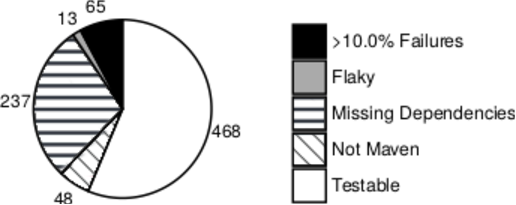
\includegraphics[width=0.27\textwidth]{results/piechart-subjs.pdf}
  \caption{\label{fig:subjects}We fetched \SubjectsGithub{} popular projects
  hosted on \github{}. From this initial sample, we ignored
  \SubjectsGithubNotMaven{} projects without Maven support,
  \SubjectsGithubNotTestable{} with missing dependencies,
  \SubjectsGithubFlaky{} projects with flaky tests, and
  \SubjectsGithubTooManyFailures{} projects had at least
  \SuiteFailingThreshold{} of failing tests. We considered
  \numSubjs{} projects to conduct our study.}
\end{figure}

\label{sec:setup}
To run our experiments, we used a Core i7-4790 (3.60 GHz) Intel processor
machine with eight virtual CPUs (four cores with two native threads each) and
16GB of memory, running Ubuntu 14.04 LTS Trusty Tahr (64-bit version).  We
used\Comment{ Git,} Java 8 and Maven 3.3.9 to build projects and run test
suites. To process test results and generate plots we used Python\Comment{ 3.4},
Bash, R and Ruby\Comment{ 2.3}.  All source artifacts are publicly available for
replication on our website~\cite{ourwebpage}.  This includes supporting
scripts\Comment{ (\eg, the scripts to run the tests and generate raw analysis
data)} and the full list of projects.


\section{Objects of Analysis}
\label{sec:subjects}

%% We evaluated the characteristics of test suites in open-source
%% development from a sample set of Java projects from \github{}.  We are
%% interested to evaluate non-trivial test suites from popular projects
%% that are in activity.

%% , which is used on
%% \github{} to indicate appreciation of a user to a
%% project~\cite{github-stars},

We used \github{}'s search API~\cite{githubsearch} to identify
projects that satisfy the following criteria: (1) the primary language
is Java\footnote{In case of projects in multiple languages, the
  \github{} API considers the predominant language as the primary
  language.}, (2) the project has at least 100 stars, (3) the latest
update was on or after January 1st, 2016, and (4) the \emph{readme}
file contains the string \emph{mvn}.  We focused on Java for its
popularity.  Although there is no clearcut limit on the number of
\github{} stars~\cite{github-stars} to define relevant projects, we
observed that 100 was enough to eliminate trivial subjects. The third
criteria serves to skip projects without recent activity. The fourth
criteria is an approximation to find Maven projects.\Comment{ The
  rationale is that if the string \emph{mvn} exists in the
  \emph{readme} file, it may represent a Maven call (\eg, to compile
  or to test the project).} We focused on Maven for its popularity on
Java projects.  Important to highlight that, as of now, the
\github{}'s search API can only reflect contents from README file (not
other code elements); it does not provide a feature to search for
projects containing certain files in the dir structure (\eg{},
\emph{pom.xml}).  Figure~\ref{fig:subject-query} illustrates the query
to the \github{} API as an HTTP request.  

\vspace{1ex}
\begin{figure}[h!]
\centering
\scriptsize
\lstset{
    escapeinside={@}{@},
    numbers=left,xleftmargin=1em,frame=single,framexleftmargin=0.5em,
    basicstyle=\ttfamily\scriptsize, boxpos=c, numberstyle=\tiny,
    deletekeywords={true}
}
\begin{lstlisting}
https://api.github.com/search/repositories?q=language:java
        +stars:>=100+pushed:>=2016-01-01
        +mvn%20in:readme+sort:stars
\end{lstlisting}
    \caption{\label{fig:subject-query} Query to the \github{} API for
    projects with the following criteria: (1) Java, (2) at least 100
    stars, (3) updated on January 1st, 2016 (or later), (4) contains
    the string \emph{mvn} in the \emph{readme} file. Output is
    paginated in descending order of stars.}
\end{figure}

After obtaining a list of potential projects, we filtered those
containing a \pomf{} file in the root directory.  A Maven project may
contain several sub-modules with multiple \pomf{} files.\Comment{  We
based our methodology to select experimental subjects on other recent
studies in testing and
debugging~\cite{gligoric-etal-issta2015,perez-etal-icst2017}.} As of
March 25th 2017, our search criteria returned \SubjectsGithub{}
subjects. Figure~\ref{fig:subjects} summarizes our sample set. 

\begin{figure}[ht]
    \centering
    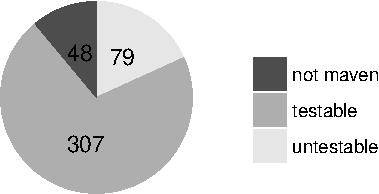
\includegraphics[width=0.25\textwidth]{plots/subjs.pdf}
    \caption{\label{fig:subjects}We fetched \SubjectsGithub{} popular projects
    hosted on \github{}. From this initial sample, we ignored
    \SubjectsGithubNotMaven{} projects without Maven support,
    \SubjectsGithubNotCompilable{} were unable to compile, and
    \SubjectsGithubNotTestable{} untestable projects\Comment{, and
    \SubjectsGithubFlaky{} projects with flaky tests}. We considered
    \numSubjs{} projects to conduct our study.}
\end{figure}

From \SubjectsGithub{} downloaded projects, \SubjectsGithubNotMaven{}
projects were not Maven or did not have a \pomf{} in the root
directory, \SubjectsGithubNotCompilable{} were unable to compile due
to missing dependencies, and \SubjectsGithubNotTestable{} projects
were untestable due to incompatible testing environment.  We also
found \SubjectsGithubFlaky{} projects with ``flaky'' tests.  We
considered those projects but ignored their tests (using JUnit's
\CodeIn{@Ignore} annotation) as to avoid measurement noise.  To detect
those projects, we executed every test suite for three times.  Our
final set of subjects consists of \numSubjs{} projects.

\subsection{Setup and Replication}
\label{sec:setup}

To run our experiments, we used a Core i7-4790 (3.60 GHz) Intel
processor machine with eight virtual CPUs (four cores with two native
threads each) and 16GB of memory, running Ubuntu 14.04 LTS Trusty Tahr
(64-bit version).  Software settings include \Comment{the Linux
  \emph{sysstat} package to measure performance, }git to fetch
subjects, Java 8, and Maven 3.3.9 to build and test subjects. We used
Python\Comment{ 3.4}, Bash, R and Ruby\Comment{ 2.3} to process the
data and generate plots.  All source artifacts are publicly available
for replication (on request)\Comment{ at \Fix{create gh-pages}}.  This
includes supporting scripts (\eg, the script that test subjects and
generates raw analysis data) and the full list of projects. \Comment{,
  and a \emph{Vagrantfile} to emulate our hardware and all software
  dependencies.}


\section{Evaluation}
\label{sec:eval}

%% We are interested in understanding the prevalence of time-consuming
%% test suites and main sources of execution cost. We want to understand
%% how the execution cost is distributed on test cases within a test
%% suite and how developers approach test execution. Based on that, we
%% study parallelization of testing frameworks and build systems.  More
%% precisely, we investigate how prevalent test parallelization is, the
%% potential for improving execution cost, issues of flakiness that
%% hinders the use of parallelization, and how to address those issues.
%% More specifically, we pose the following research questions:

%% The first research question addresses the prevalence of long-running
%% test suites. We are interested to know if costly test suites are
%% common in open-source projects.  The second research question
%% addresses the relationship of test cases and the overall execution
%% cost: we are interested to investigate how the execution time is
%% distributed among test cases.  In the third research question, we
%% investigate if developers consider low-level parallelism features
%% available out-of-the-box to amortize test execution (see
%% Section~\ref{sec:modes}). In addition, we want to identify what
%% configurations are often used and why they are more popular (if any).
%% The fourth research question addresses the impact of low-level
%% parallelism on test execution from projects in our sample set. We want
%% to identify subjects that already use test parallelization and compare
%% their performance in contrast to sequential execution. In addition, we
%% are interested in evaluating the performance of sequential test suites
%% with different parallelization settings.
%% Finally, the fifth research question discusses the limitations and
%% insights to overcome the pitfalls of parallelization.

%% \Comment{
%%     \Fix{distribution of execution time per test case. For each subject
%%     identified in the first research question, we investigate how
%%     balanced is the cost of the test suite in contrast to the cost of
%%     test cases and if there are subjects where the time cost is mostly
%%     dominated by a small fraction of test cases.} \Fix{The third research
%%     question addresses the distribution of regression tests according
%%     to the use of computational resources.  We are interested in
%%     investigating if regression test suites are CPU intensive and if there
%%     are opportunities to improve performance. The RQ4 addresses}
%%     \Fix{...elaborate...}

%%     The rationale is that if the time cost of a regression test is equally
%%     distributed among test cases, the execution cost could be potentially
%%     improved by running tests in parallel (in contrast to the scenario
%%     where only one test case dominates most of the execution time).
%% }

We pose the following research questions, organized by the dimensions
of analysis we presented in Section~\ref{sec:intro}.


%% Feasibility
\newcommand{\numRQFeasibilityOne}{RQ1}
\newcommand{\RQFeasibilityOne}{How prevalent is the occurence of time-consuming
  test suites\Comment{ in open-source projects}?}

\newcommand{\numRQFeasibilityTwo}{RQ2}
\newcommand{\RQFeasibilityTwo}{How time is distributed across test cases?}

%% Adoption
\newcommand{\numRQAdoptionOne}{RQ3}
\newcommand{\RQAdoptionOne}{How popular is test suite
  parallelization\Comment{ in open-source projects}?}

\newcommand{\numRQAdoptionTwo}{RQ4}
\newcommand{\RQAdoptionTwo}{What are the main reasons that prevent developers
  from using test suite parallelization?}

%% Speedups
\newcommand{\numRQSpeedupOne}{RQ5}
\newcommand{\RQSpeedupOne}{What are the speedups obtained with parallelization
  (in projects that actually use it)?}

\newcommand{\numRQSpeedupTwo}{RQ6}
\newcommand{\RQSpeedupTwo}{How test execution scales with the number of
  available CPUs?}

%% Issues
\newcommand{\numRQIssuesOne}{RQ7}
\newcommand{\RQIssuesOne}{How parallel execution configurations affect testing
  costs and flakiness?}


\setlist[itemize]{leftmargin=1em}
\begin{itemize}
\item Feasibility
  \begin{itemize}
  \item \textbf{\numRQFeasibilityOne.} \RQFeasibilityOne
  \item \textbf{\numRQFeasibilityTwo.} \RQFeasibilityTwo    
  \end{itemize}
\item Adoption
  \begin{itemize}
  \item \textbf{\numRQAdoptionOne.} \RQAdoptionOne    
  \item \textbf{\numRQAdoptionTwo.} \RQAdoptionTwo
  \end{itemize}
\item Speedups
  \begin{itemize}
  \item \textbf{\numRQSpeedupOne.} \RQSpeedupOne
  \item \textbf{\numRQSpeedupTwo.} \RQSpeedupTwo
  \end{itemize}      
\item Issues
  \begin{itemize}
  \item \textbf{\numRQIssuesOne.} \RQIssuesOne    
  \end{itemize}
\end{itemize}

%%\newcommand{\RQFeasibilityTwo}{What is the distribution of CPU and IO bound
%%regression test suites from the sample set?}
%%
%%\newcommand{\RQAdoptionOne}{How uniformly distributed is the execution time
%%across test cases in costly projects?}
%%
%%\newcommand{\RQAdoptionTwo}{How often developers use the parallelism features
%%from build systems to improve runtime performance?}



\subsection{Feasibility}
\label{sec:rqA}
\label{sec:rqB}

\begin{itemize}
    \item \numRQFeasibilityOne{}. \textbf{\RQFeasibilityOne}
\end{itemize}
%\Jbc{The following steps may change $\rightarrow$}

To evaluate prevalence of projects with costly test suites, we
considered the \numSubjs{} testable subjects from
Figure~\ref{fig:subjects}.  Figure~\ref{fig:mvn-execution} illustrates
the script we used to measure time.

We took the following actions to isolate our environment from
measurement noise.  First, we observed that some test tasks called
test-unrelated tasks (\eg, \emph{javadoc} generation and static
analyses) that could interfere in our time measurements.  To address
that potential issue, we inspected Maven execution logs from a sample
including a hundred projects prior to running the script from
Figure~\ref{fig:mvn-execution}.  The tasks we found were ignored from
execution (lines 1-3).  Furthermore, to avoid noise from operating
system events, we configured our workstation to run only essential
services.  The machine was dedicated to our experiments and we
accessed it via SSH. In addition, we configured the \CodeIn{isolcpus}
option from the Linux Kernel \cite{linux-kernel} to isolate six
virtual CPUs to run our experiments, leaving the remaining CPUs to run
OS processes~\cite{isolcpus-use}.  The rationale for this decision is
to prevent context-switching between user processes (running the
experiment) and OS-related processes.  Finally, to make sure our
measurements were fair, we compared timings corresponding to the
sequential execution of tests using Maven with that obtained with
JUnit's default \CodeIn{JUnitCore} runner, invoked from the command
line.  Results were very close.

The main loop (lines 5-11) of the script in
Figure~\ref{fig:mvn-execution} iterates over the list of subjects and
invokes Maven multiple times\Comment{ to isolate cost of running
  tests} (lines 7-9).  It first compiles the source and test files
(line 7), make all dependencies available locally (line 8), and then
runs the tests in offline mode as to skip the package update task,
enabled by default (line 9). After execution, we used a regular
expression on the output log to extract elapsed time (line 10).

%% We executed each project's test suite for
%% \Fix{5} times through Maven and directly through JUnit each project

\section{Objects of Analysis}
\label{sec:subjects}

%% We evaluated the characteristics of test suites in open-source
%% development from a sample set of Java projects from \github{}.  We are
%% interested to evaluate non-trivial test suites from popular projects
%% that are in activity.

%% , which is used on
%% \github{} to indicate appreciation of a user to a
%% project~\cite{github-stars},

We used \github{}'s search API~\cite{githubsearch} to identify
projects that satisfy the following criteria: (1) the primary language
is Java\footnote{In case of projects in multiple languages, the
  \github{} API considers the predominant language as the primary
  language.}, (2) the project has at least 100 stars, (3) the latest
update was on or after January 1st, 2016, and (4) the \emph{readme}
file contains the string \emph{mvn}.  We focused on Java for its
popularity.  Although there is no clearcut limit on the number of
\github{} stars~\cite{github-stars} to define relevant projects, we
observed that 100 was enough to eliminate trivial subjects. The third
criteria serves to skip projects without recent activity. The fourth
criteria is an approximation to find Maven projects.\Comment{ The
  rationale is that if the string \emph{mvn} exists in the
  \emph{readme} file, it may represent a Maven call (\eg, to compile
  or to test the project).} We focused on Maven for its popularity on
Java projects.  Important to highlight that, as of now, the
\github{}'s search API can only reflect contents from README file (not
other code elements); it does not provide a feature to search for
projects containing certain files in the dir structure (\eg{},
\emph{pom.xml}).  Figure~\ref{fig:subject-query} illustrates the query
to the \github{} API as an HTTP request.  

\vspace{1ex}
\begin{figure}[h!]
\centering
\scriptsize
\lstset{
    escapeinside={@}{@},
    numbers=left,xleftmargin=1em,frame=single,framexleftmargin=0.5em,
    basicstyle=\ttfamily\scriptsize, boxpos=c, numberstyle=\tiny,
    deletekeywords={true}
}
\begin{lstlisting}
https://api.github.com/search/repositories?q=language:java
        +stars:>=100+pushed:>=2016-01-01
        +mvn%20in:readme+sort:stars
\end{lstlisting}
    \caption{\label{fig:subject-query} Query to the \github{} API for
    projects with the following criteria: (1) Java, (2) at least 100
    stars, (3) updated on January 1st, 2016 (or later), (4) contains
    the string \emph{mvn} in the \emph{readme} file. Output is
    paginated in descending order of stars.}
\end{figure}

After obtaining a list of potential projects, we filtered those
containing a \pomf{} file in the root directory.  A Maven project may
contain several sub-modules with multiple \pomf{} files.\Comment{  We
based our methodology to select experimental subjects on other recent
studies in testing and
debugging~\cite{gligoric-etal-issta2015,perez-etal-icst2017}.} As of
March 25th 2017, our search criteria returned \SubjectsGithub{}
subjects. Figure~\ref{fig:subjects} summarizes our sample set. 

\begin{figure}[ht]
    \centering
    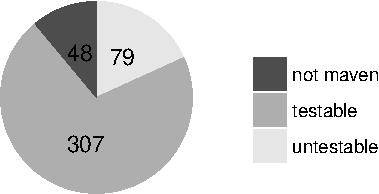
\includegraphics[width=0.25\textwidth]{plots/subjs.pdf}
    \caption{\label{fig:subjects}We fetched \SubjectsGithub{} popular projects
    hosted on \github{}. From this initial sample, we ignored
    \SubjectsGithubNotMaven{} projects without Maven support,
    \SubjectsGithubNotCompilable{} were unable to compile, and
    \SubjectsGithubNotTestable{} untestable projects\Comment{, and
    \SubjectsGithubFlaky{} projects with flaky tests}. We considered
    \numSubjs{} projects to conduct our study.}
\end{figure}

From \SubjectsGithub{} downloaded projects, \SubjectsGithubNotMaven{}
projects were not Maven or did not have a \pomf{} in the root
directory, \SubjectsGithubNotCompilable{} were unable to compile due
to missing dependencies, and \SubjectsGithubNotTestable{} projects
were untestable due to incompatible testing environment.  We also
found \SubjectsGithubFlaky{} projects with ``flaky'' tests.  We
considered those projects but ignored their tests (using JUnit's
\CodeIn{@Ignore} annotation) as to avoid measurement noise.  To detect
those projects, we executed every test suite for three times.  Our
final set of subjects consists of \numSubjs{} projects.

\subsection{Setup and Replication}
\label{sec:setup}

To run our experiments, we used a Core i7-4790 (3.60 GHz) Intel
processor machine with eight virtual CPUs (four cores with two native
threads each) and 16GB of memory, running Ubuntu 14.04 LTS Trusty Tahr
(64-bit version).  Software settings include \Comment{the Linux
  \emph{sysstat} package to measure performance, }git to fetch
subjects, Java 8, and Maven 3.3.9 to build and test subjects. We used
Python\Comment{ 3.4}, Bash, R and Ruby\Comment{ 2.3} to process the
data and generate plots.  All source artifacts are publicly available
for replication (on request)\Comment{ at \Fix{create gh-pages}}.  This
includes supporting scripts (\eg, the script that test subjects and
generates raw analysis data) and the full list of projects. \Comment{,
  and a \emph{Vagrantfile} to emulate our hardware and all software
  dependencies.}


\section{Evaluation}
\label{sec:eval}

%% We are interested in understanding the prevalence of time-consuming
%% test suites and main sources of execution cost. We want to understand
%% how the execution cost is distributed on test cases within a test
%% suite and how developers approach test execution. Based on that, we
%% study parallelization of testing frameworks and build systems.  More
%% precisely, we investigate how prevalent test parallelization is, the
%% potential for improving execution cost, issues of flakiness that
%% hinders the use of parallelization, and how to address those issues.
%% More specifically, we pose the following research questions:

%% The first research question addresses the prevalence of long-running
%% test suites. We are interested to know if costly test suites are
%% common in open-source projects.  The second research question
%% addresses the relationship of test cases and the overall execution
%% cost: we are interested to investigate how the execution time is
%% distributed among test cases.  In the third research question, we
%% investigate if developers consider low-level parallelism features
%% available out-of-the-box to amortize test execution (see
%% Section~\ref{sec:modes}). In addition, we want to identify what
%% configurations are often used and why they are more popular (if any).
%% The fourth research question addresses the impact of low-level
%% parallelism on test execution from projects in our sample set. We want
%% to identify subjects that already use test parallelization and compare
%% their performance in contrast to sequential execution. In addition, we
%% are interested in evaluating the performance of sequential test suites
%% with different parallelization settings.
%% Finally, the fifth research question discusses the limitations and
%% insights to overcome the pitfalls of parallelization.

%% \Comment{
%%     \Fix{distribution of execution time per test case. For each subject
%%     identified in the first research question, we investigate how
%%     balanced is the cost of the test suite in contrast to the cost of
%%     test cases and if there are subjects where the time cost is mostly
%%     dominated by a small fraction of test cases.} \Fix{The third research
%%     question addresses the distribution of regression tests according
%%     to the use of computational resources.  We are interested in
%%     investigating if regression test suites are CPU intensive and if there
%%     are opportunities to improve performance. The RQ4 addresses}
%%     \Fix{...elaborate...}

%%     The rationale is that if the time cost of a regression test is equally
%%     distributed among test cases, the execution cost could be potentially
%%     improved by running tests in parallel (in contrast to the scenario
%%     where only one test case dominates most of the execution time).
%% }

We pose the following research questions, organized by the dimensions
of analysis we presented in Section~\ref{sec:intro}.


%% Feasibility
\newcommand{\numRQFeasibilityOne}{RQ1}
\newcommand{\RQFeasibilityOne}{How prevalent is the occurence of time-consuming
  test suites\Comment{ in open-source projects}?}

\newcommand{\numRQFeasibilityTwo}{RQ2}
\newcommand{\RQFeasibilityTwo}{How time is distributed across test cases?}

%% Adoption
\newcommand{\numRQAdoptionOne}{RQ3}
\newcommand{\RQAdoptionOne}{How popular is test suite
  parallelization\Comment{ in open-source projects}?}

\newcommand{\numRQAdoptionTwo}{RQ4}
\newcommand{\RQAdoptionTwo}{What are the main reasons that prevent developers
  from using test suite parallelization?}

%% Speedups
\newcommand{\numRQSpeedupOne}{RQ5}
\newcommand{\RQSpeedupOne}{What are the speedups obtained with parallelization
  (in projects that actually use it)?}

\newcommand{\numRQSpeedupTwo}{RQ6}
\newcommand{\RQSpeedupTwo}{How test execution scales with the number of
  available CPUs?}

%% Issues
\newcommand{\numRQIssuesOne}{RQ7}
\newcommand{\RQIssuesOne}{How parallel execution configurations affect testing
  costs and flakiness?}


\setlist[itemize]{leftmargin=1em}
\begin{itemize}
\item Feasibility
  \begin{itemize}
  \item \textbf{\numRQFeasibilityOne.} \RQFeasibilityOne
  \item \textbf{\numRQFeasibilityTwo.} \RQFeasibilityTwo    
  \end{itemize}
\item Adoption
  \begin{itemize}
  \item \textbf{\numRQAdoptionOne.} \RQAdoptionOne    
  \item \textbf{\numRQAdoptionTwo.} \RQAdoptionTwo
  \end{itemize}
\item Speedups
  \begin{itemize}
  \item \textbf{\numRQSpeedupOne.} \RQSpeedupOne
  \item \textbf{\numRQSpeedupTwo.} \RQSpeedupTwo
  \end{itemize}      
\item Issues
  \begin{itemize}
  \item \textbf{\numRQIssuesOne.} \RQIssuesOne    
  \end{itemize}
\end{itemize}

%%\newcommand{\RQFeasibilityTwo}{What is the distribution of CPU and IO bound
%%regression test suites from the sample set?}
%%
%%\newcommand{\RQAdoptionOne}{How uniformly distributed is the execution time
%%across test cases in costly projects?}
%%
%%\newcommand{\RQAdoptionTwo}{How often developers use the parallelism features
%%from build systems to improve runtime performance?}



\subsection{Feasibility}
\label{sec:rqA}
\label{sec:rqB}

\begin{itemize}
    \item \numRQFeasibilityOne{}. \textbf{\RQFeasibilityOne}
\end{itemize}
%\Jbc{The following steps may change $\rightarrow$}

To evaluate prevalence of projects with costly test suites, we
considered the \numSubjs{} testable subjects from
Figure~\ref{fig:subjects}.  Figure~\ref{fig:mvn-execution} illustrates
the script we used to measure time.

We took the following actions to isolate our environment from
measurement noise.  First, we observed that some test tasks called
test-unrelated tasks (\eg, \emph{javadoc} generation and static
analyses) that could interfere in our time measurements.  To address
that potential issue, we inspected Maven execution logs from a sample
including a hundred projects prior to running the script from
Figure~\ref{fig:mvn-execution}.  The tasks we found were ignored from
execution (lines 1-3).  Furthermore, to avoid noise from operating
system events, we configured our workstation to run only essential
services.  The machine was dedicated to our experiments and we
accessed it via SSH. In addition, we configured the \CodeIn{isolcpus}
option from the Linux Kernel \cite{linux-kernel} to isolate six
virtual CPUs to run our experiments, leaving the remaining CPUs to run
OS processes~\cite{isolcpus-use}.  The rationale for this decision is
to prevent context-switching between user processes (running the
experiment) and OS-related processes.  Finally, to make sure our
measurements were fair, we compared timings corresponding to the
sequential execution of tests using Maven with that obtained with
JUnit's default \CodeIn{JUnitCore} runner, invoked from the command
line.  Results were very close.

The main loop (lines 5-11) of the script in
Figure~\ref{fig:mvn-execution} iterates over the list of subjects and
invokes Maven multiple times\Comment{ to isolate cost of running
  tests} (lines 7-9).  It first compiles the source and test files
(line 7), make all dependencies available locally (line 8), and then
runs the tests in offline mode as to skip the package update task,
enabled by default (line 9). After execution, we used a regular
expression on the output log to extract elapsed time (line 10).

%% We executed each project's test suite for
%% \Fix{5} times through Maven and directly through JUnit each project

\section{Objects of Analysis}
\label{sec:subjects}

%% We evaluated the characteristics of test suites in open-source
%% development from a sample set of Java projects from \github{}.  We are
%% interested to evaluate non-trivial test suites from popular projects
%% that are in activity.

%% , which is used on
%% \github{} to indicate appreciation of a user to a
%% project~\cite{github-stars},

We used \github{}'s search API~\cite{githubsearch} to identify
projects that satisfy the following criteria: (1) the primary language
is Java\footnote{In case of projects in multiple languages, the
  \github{} API considers the predominant language as the primary
  language.}, (2) the project has at least 100 stars, (3) the latest
update was on or after January 1st, 2016, and (4) the \emph{readme}
file contains the string \emph{mvn}.  We focused on Java for its
popularity.  Although there is no clearcut limit on the number of
\github{} stars~\cite{github-stars} to define relevant projects, we
observed that 100 was enough to eliminate trivial subjects. The third
criteria serves to skip projects without recent activity. The fourth
criteria is an approximation to find Maven projects.\Comment{ The
  rationale is that if the string \emph{mvn} exists in the
  \emph{readme} file, it may represent a Maven call (\eg, to compile
  or to test the project).} We focused on Maven for its popularity on
Java projects.  Important to highlight that, as of now, the
\github{}'s search API can only reflect contents from README file (not
other code elements); it does not provide a feature to search for
projects containing certain files in the dir structure (\eg{},
\emph{pom.xml}).  Figure~\ref{fig:subject-query} illustrates the query
to the \github{} API as an HTTP request.  

\vspace{1ex}
\begin{figure}[h!]
\centering
\scriptsize
\lstset{
    escapeinside={@}{@},
    numbers=left,xleftmargin=1em,frame=single,framexleftmargin=0.5em,
    basicstyle=\ttfamily\scriptsize, boxpos=c, numberstyle=\tiny,
    deletekeywords={true}
}
\begin{lstlisting}
https://api.github.com/search/repositories?q=language:java
        +stars:>=100+pushed:>=2016-01-01
        +mvn%20in:readme+sort:stars
\end{lstlisting}
    \caption{\label{fig:subject-query} Query to the \github{} API for
    projects with the following criteria: (1) Java, (2) at least 100
    stars, (3) updated on January 1st, 2016 (or later), (4) contains
    the string \emph{mvn} in the \emph{readme} file. Output is
    paginated in descending order of stars.}
\end{figure}

After obtaining a list of potential projects, we filtered those
containing a \pomf{} file in the root directory.  A Maven project may
contain several sub-modules with multiple \pomf{} files.\Comment{  We
based our methodology to select experimental subjects on other recent
studies in testing and
debugging~\cite{gligoric-etal-issta2015,perez-etal-icst2017}.} As of
March 25th 2017, our search criteria returned \SubjectsGithub{}
subjects. Figure~\ref{fig:subjects} summarizes our sample set. 

\begin{figure}[ht]
    \centering
    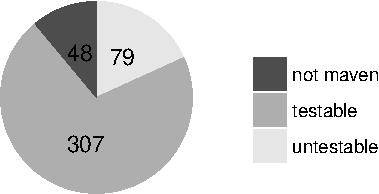
\includegraphics[width=0.25\textwidth]{plots/subjs.pdf}
    \caption{\label{fig:subjects}We fetched \SubjectsGithub{} popular projects
    hosted on \github{}. From this initial sample, we ignored
    \SubjectsGithubNotMaven{} projects without Maven support,
    \SubjectsGithubNotCompilable{} were unable to compile, and
    \SubjectsGithubNotTestable{} untestable projects\Comment{, and
    \SubjectsGithubFlaky{} projects with flaky tests}. We considered
    \numSubjs{} projects to conduct our study.}
\end{figure}

From \SubjectsGithub{} downloaded projects, \SubjectsGithubNotMaven{}
projects were not Maven or did not have a \pomf{} in the root
directory, \SubjectsGithubNotCompilable{} were unable to compile due
to missing dependencies, and \SubjectsGithubNotTestable{} projects
were untestable due to incompatible testing environment.  We also
found \SubjectsGithubFlaky{} projects with ``flaky'' tests.  We
considered those projects but ignored their tests (using JUnit's
\CodeIn{@Ignore} annotation) as to avoid measurement noise.  To detect
those projects, we executed every test suite for three times.  Our
final set of subjects consists of \numSubjs{} projects.

\subsection{Setup and Replication}
\label{sec:setup}

To run our experiments, we used a Core i7-4790 (3.60 GHz) Intel
processor machine with eight virtual CPUs (four cores with two native
threads each) and 16GB of memory, running Ubuntu 14.04 LTS Trusty Tahr
(64-bit version).  Software settings include \Comment{the Linux
  \emph{sysstat} package to measure performance, }git to fetch
subjects, Java 8, and Maven 3.3.9 to build and test subjects. We used
Python\Comment{ 3.4}, Bash, R and Ruby\Comment{ 2.3} to process the
data and generate plots.  All source artifacts are publicly available
for replication (on request)\Comment{ at \Fix{create gh-pages}}.  This
includes supporting scripts (\eg, the script that test subjects and
generates raw analysis data) and the full list of projects. \Comment{,
  and a \emph{Vagrantfile} to emulate our hardware and all software
  dependencies.}


\section{Evaluation}
\label{sec:eval}

%% We are interested in understanding the prevalence of time-consuming
%% test suites and main sources of execution cost. We want to understand
%% how the execution cost is distributed on test cases within a test
%% suite and how developers approach test execution. Based on that, we
%% study parallelization of testing frameworks and build systems.  More
%% precisely, we investigate how prevalent test parallelization is, the
%% potential for improving execution cost, issues of flakiness that
%% hinders the use of parallelization, and how to address those issues.
%% More specifically, we pose the following research questions:

%% The first research question addresses the prevalence of long-running
%% test suites. We are interested to know if costly test suites are
%% common in open-source projects.  The second research question
%% addresses the relationship of test cases and the overall execution
%% cost: we are interested to investigate how the execution time is
%% distributed among test cases.  In the third research question, we
%% investigate if developers consider low-level parallelism features
%% available out-of-the-box to amortize test execution (see
%% Section~\ref{sec:modes}). In addition, we want to identify what
%% configurations are often used and why they are more popular (if any).
%% The fourth research question addresses the impact of low-level
%% parallelism on test execution from projects in our sample set. We want
%% to identify subjects that already use test parallelization and compare
%% their performance in contrast to sequential execution. In addition, we
%% are interested in evaluating the performance of sequential test suites
%% with different parallelization settings.
%% Finally, the fifth research question discusses the limitations and
%% insights to overcome the pitfalls of parallelization.

%% \Comment{
%%     \Fix{distribution of execution time per test case. For each subject
%%     identified in the first research question, we investigate how
%%     balanced is the cost of the test suite in contrast to the cost of
%%     test cases and if there are subjects where the time cost is mostly
%%     dominated by a small fraction of test cases.} \Fix{The third research
%%     question addresses the distribution of regression tests according
%%     to the use of computational resources.  We are interested in
%%     investigating if regression test suites are CPU intensive and if there
%%     are opportunities to improve performance. The RQ4 addresses}
%%     \Fix{...elaborate...}

%%     The rationale is that if the time cost of a regression test is equally
%%     distributed among test cases, the execution cost could be potentially
%%     improved by running tests in parallel (in contrast to the scenario
%%     where only one test case dominates most of the execution time).
%% }

We pose the following research questions, organized by the dimensions
of analysis we presented in Section~\ref{sec:intro}.


%% Feasibility
\newcommand{\numRQFeasibilityOne}{RQ1}
\newcommand{\RQFeasibilityOne}{How prevalent is the occurence of time-consuming
  test suites\Comment{ in open-source projects}?}

\newcommand{\numRQFeasibilityTwo}{RQ2}
\newcommand{\RQFeasibilityTwo}{How time is distributed across test cases?}

%% Adoption
\newcommand{\numRQAdoptionOne}{RQ3}
\newcommand{\RQAdoptionOne}{How popular is test suite
  parallelization\Comment{ in open-source projects}?}

\newcommand{\numRQAdoptionTwo}{RQ4}
\newcommand{\RQAdoptionTwo}{What are the main reasons that prevent developers
  from using test suite parallelization?}

%% Speedups
\newcommand{\numRQSpeedupOne}{RQ5}
\newcommand{\RQSpeedupOne}{What are the speedups obtained with parallelization
  (in projects that actually use it)?}

\newcommand{\numRQSpeedupTwo}{RQ6}
\newcommand{\RQSpeedupTwo}{How test execution scales with the number of
  available CPUs?}

%% Issues
\newcommand{\numRQIssuesOne}{RQ7}
\newcommand{\RQIssuesOne}{How parallel execution configurations affect testing
  costs and flakiness?}


\setlist[itemize]{leftmargin=1em}
\begin{itemize}
\item Feasibility
  \begin{itemize}
  \item \textbf{\numRQFeasibilityOne.} \RQFeasibilityOne
  \item \textbf{\numRQFeasibilityTwo.} \RQFeasibilityTwo    
  \end{itemize}
\item Adoption
  \begin{itemize}
  \item \textbf{\numRQAdoptionOne.} \RQAdoptionOne    
  \item \textbf{\numRQAdoptionTwo.} \RQAdoptionTwo
  \end{itemize}
\item Speedups
  \begin{itemize}
  \item \textbf{\numRQSpeedupOne.} \RQSpeedupOne
  \item \textbf{\numRQSpeedupTwo.} \RQSpeedupTwo
  \end{itemize}      
\item Issues
  \begin{itemize}
  \item \textbf{\numRQIssuesOne.} \RQIssuesOne    
  \end{itemize}
\end{itemize}

%%\newcommand{\RQFeasibilityTwo}{What is the distribution of CPU and IO bound
%%regression test suites from the sample set?}
%%
%%\newcommand{\RQAdoptionOne}{How uniformly distributed is the execution time
%%across test cases in costly projects?}
%%
%%\newcommand{\RQAdoptionTwo}{How often developers use the parallelism features
%%from build systems to improve runtime performance?}



\subsection{Feasibility}
\label{sec:rqA}
\label{sec:rqB}

\begin{itemize}
    \item \numRQFeasibilityOne{}. \textbf{\RQFeasibilityOne}
\end{itemize}
%\Jbc{The following steps may change $\rightarrow$}

To evaluate prevalence of projects with costly test suites, we
considered the \numSubjs{} testable subjects from
Figure~\ref{fig:subjects}.  Figure~\ref{fig:mvn-execution} illustrates
the script we used to measure time.

We took the following actions to isolate our environment from
measurement noise.  First, we observed that some test tasks called
test-unrelated tasks (\eg, \emph{javadoc} generation and static
analyses) that could interfere in our time measurements.  To address
that potential issue, we inspected Maven execution logs from a sample
including a hundred projects prior to running the script from
Figure~\ref{fig:mvn-execution}.  The tasks we found were ignored from
execution (lines 1-3).  Furthermore, to avoid noise from operating
system events, we configured our workstation to run only essential
services.  The machine was dedicated to our experiments and we
accessed it via SSH. In addition, we configured the \CodeIn{isolcpus}
option from the Linux Kernel \cite{linux-kernel} to isolate six
virtual CPUs to run our experiments, leaving the remaining CPUs to run
OS processes~\cite{isolcpus-use}.  The rationale for this decision is
to prevent context-switching between user processes (running the
experiment) and OS-related processes.  Finally, to make sure our
measurements were fair, we compared timings corresponding to the
sequential execution of tests using Maven with that obtained with
JUnit's default \CodeIn{JUnitCore} runner, invoked from the command
line.  Results were very close.

The main loop (lines 5-11) of the script in
Figure~\ref{fig:mvn-execution} iterates over the list of subjects and
invokes Maven multiple times\Comment{ to isolate cost of running
  tests} (lines 7-9).  It first compiles the source and test files
(line 7), make all dependencies available locally (line 8), and then
runs the tests in offline mode as to skip the package update task,
enabled by default (line 9). After execution, we used a regular
expression on the output log to extract elapsed time (line 10).

%% We executed each project's test suite for
%% \Fix{5} times through Maven and directly through JUnit each project

\input{codes/evaluation}

We ran the test suite for each subject three times, reporting averaged
execution times in three ranges: tests that run within a minute
(\shortg{} group), tests that run in one to five minutes (\medg{}
group), and tests that run in five or more minutes (\longg{}
group). We followed a similar methodology to group projects by time as
Gligoric~\etal{}~\cite{gligoric-etal-issta2015} in their work on
regression test selection.\Comment{ and added the \medg{} group due to
  the variability of the time cost from subjects out of the \shortg{}
  group} Figure~\ref{fig:rq1-barplot} shows the number of projects in
each group.  As expected, \longg{} and \medg{} projects do not occur
as frequently as \shortg{} projects.  However, they do occur in
relatively high numbers.

Figure~\ref{fig:rq1-boxplot} shows cost distribution of test suites in
each group as boxplots.  Note that the y-ranges are different.  The
distribution associated with the \shortg{} group is the most
unbalanced (right skewed)\Comment{ with outliers closed to the \medg{}
  group}.  The test suites in this group ran in 15 or less seconds for
over 75\% of the cases.  Such scenarios constitute the majority of the
cases we analyzed.  Considering the groups \medg{} and \longg{},
however, we found many costly executions.  Nearly 75\% of the projects
from the \medg{} group take over 3.5 minutes to run and nearly 75\% of
the projects from the \longg{} group take $\sim$20 minutes to run.  We
found cases in the \longg{} group were execution takes over 50 minutes
to complete, as can be observed from the outliers (dots) in the plot.

%% the median from the
%% \medg{} group is nearly two minutes and most of the subjects run in
%% less than four minutes; most of the \longg{} group runs in less than
%% 25 minutes but has outliers that require more than 50 minutes to
%% execute.



\begin{figure}[ht]
    \centering
    \begin{subfigure}{0.182\textwidth}
        \centering
        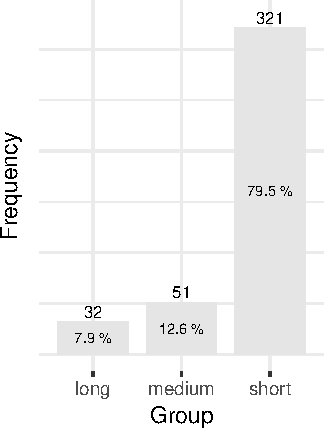
\includegraphics[width=\textwidth]{plots/barplot-timecost.pdf}
        \caption{\label{fig:rq1-barplot}}
    \end{subfigure}%
    ~
    \begin{subfigure}{0.25\textwidth}
        \centering
        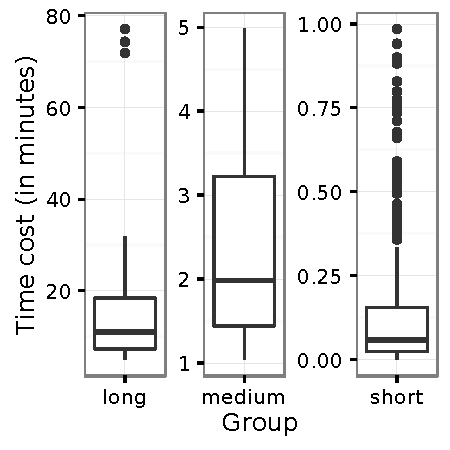
\includegraphics[width=\textwidth]{plots/boxplot-timecost.pdf}
        \caption{\label{fig:rq1-boxplot}}
    \end{subfigure}%
    \caption{(a) Subjects grouped by time cost ($t$): short run ($t <
    1m$), medium run ($1m \le t < 5m$), and long run ($5m \le t$); (b)
    Distribution of time cost by group.}
\end{figure}

%% Figure~\ref{fig:rq1-barplot} is a lower bound estimation of cost
%% because some tests may finish earlier than expected due to existing
%% test failures in the revision we downloaded.

It is important to note that we under-estimated cost in our
experiments for two main reasons.  First, some tests may finish
earlier than expected due to the observed test failures in some of the
revisions we downloaded.  From the \numSubjs{} testable projects,
\numSubjsPass{} successfully executed all tests and \numSubjsFail{}
reported some test failures.  Second, some projects may omit
long-running tests on their default execution. For instance, the
project \CodeIn{apache.maven-surefire} runs all unit tests in a few
seconds.  According to our criteria, this project is to be classified
as \shortg{} but a closer look reveals that only smoke tests are run
by default in this project.  Time-consuming integration and system
tests are only accessible via custom parameters, which we do not
handle in our experimental setup.  We enabled such parameters for this
specific project and observed that testing time goes to nearly 30
minutes.  For simplicity, we considered only the tests executed by
default.

\vspace{1ex}
\begin{center}
\fbox{
\begin{minipage}{8cm}
    \textit{Answering \numRQFeasibilityOne{}:}~\emph{We conclude that
      time-consuming test suites are relatively frequent in
      open-source projects.  We found that \percentMedLongRunning{} of
      the \numSubjs{} projects we analyzed (\ie{}, over 1 in every 5
      projects) take at least 3 minutes to run and
      \percentLongRunning{} take at least 5 minutes to run.\Comment{
        (\ie, \numMedLong{} projects from \medg{} and \longg{}).}}
\end{minipage}
}
\end{center}
\vspace{1ex}


\begin{itemize}
    \item \numRQFeasibilityTwo. \textbf{\RQFeasibilityTwo}
\end{itemize}

Section~\ref{sec:rqA} showed that medium and long-running projects are
not uncommon, accounting to nearly \percentMedLongRunning{} of the
\numSubjs{} projects we analyzed.  Research question \numRQFeasibilityTwo{}
measures the distribution of test costs in test suites as to estimate
(lack of) potential of obtaining speedups with parallelization.  In
the limit, if cost is dominated by a single test from a large test
suite, it is unlikely that parallelization will be beneficial as a
test method is the smallest working unit in test frameworks.

%% However, avoiding
%% frequent context switches is another factor to consider.  For example,
%% assuming there are at least two CPUs available for execution, cost can
%% be cut in half if two tests in a large test suite dominate execution
%% time and these tests are assigned to different CPUs.

%% It is therefore important to
%% speedup regressing testing in open-source projects.\Comment{not only
%%   to huge projects as those from Google~\cite{google-tap,google-ci}
%%   and Microsoft~\cite{prasad-shulte-ieee-microsoft-ci}.}



%% For the case
%% where cost is distributed more evenly across test cases, one expects
%% that speedups will be a function of the number of cores.
%% These contradictory forces, pushing number of tests and cost
%% of each test up and down, make prediction of effectiveness challenging.

\begin{figure}[h]
    \centering
    \begin{subfigure}{0.47\textwidth}
      \centering
      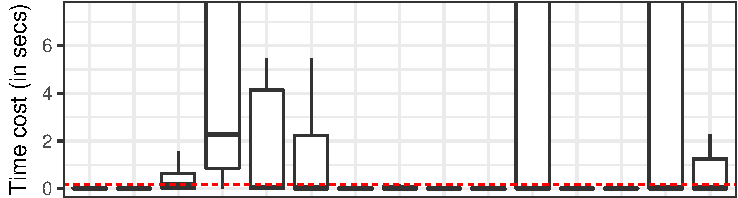
\includegraphics[width=\textwidth]{plots/testcost-long.pdf}
      \caption{\label{fig:longtcost}Long group.}
    \end{subfigure}\\
    \vspace{2ex}
    \begin{subfigure}{0.47\textwidth}
      \centering
      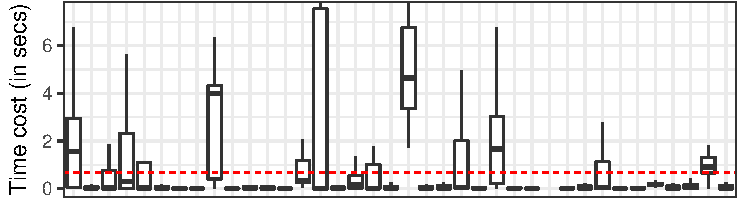
\includegraphics[width=\textwidth]{plots/testcost-medium.pdf}
      \caption{\label{fig:medtcost}Medium group.}
    \end{subfigure}
    %% \vspace{2ex}
    %% \begin{subfigure}{0.5\textwidth}
    %%   \centering
    %%   \begin{tabular}{rrrr}
    %%     \toprule
    %%     & $\sigma\leq1$ & $1<\sigma\leq5$ & $\sigma\ge5$ \\
    %%     \midrule    
    %%     Long   &  7 & 15 & 12 \\
    %%     Medium & 22 & 19 & 7 \\
    %%     \bottomrule
    %%   \end{tabular}
    %%   \caption{\label{fig:sd}Standard deviation ($\sigma$) of test case running times.}
    %% \end{subfigure}
    \caption{\label{fig:time-distributions}Time distributions.}%
\end{figure}

\sloppy Figures~\ref{fig:longtcost} and~\ref{fig:medtcost} show the
time distribution of individual test cases per project.  We observed
that the average median value of execution cost for a test was
relatively small (dashed horizontal red lines), namely 0.31s for
\medg{} projects and 0.23s for \longg{} projects.  The standard
deviations associated with each distribution were relatively
low.\Comment{ Figure~\ref{fig:sd} shows the number of projects within
  specific ranges of $\sigma$ values.}  We noted a small number of
cases of CPU monopolization.  For example, the highest value of
$\sigma$ occurred in \CodeIn{uber\_chaperone}, a project from the
medium group.  This project contains only 65 tests, 62 of which take
less than 0.5s to run, one of which takes nearly 3s to run, and two of
which take $\sim$40m to run.  For this project, 99.2\% of the
execution cost is dominated by only 3\% of the tests; without these
two costly tests this project would have been classified as
short-running.  A closer inspection in the data indicates that the
project \CodeIn{uber\_chaperone} was a corner case; we did not find
other projects with such extreme time monopolization profile.  Project
\CodeIn{facebookarchive\_linkbench} is also classified as long-running
and has the second highest value of $\sigma$.  For this project,
however, cost is distributed more smoothly across \Fix{529} tests, of
which \Fix{119 (23\%)} take more than \Fix{1s} to run with the rest of
the tests running faster.

\begin{figure}[t]
  \centering
  \begin{subfigure}{0.15\textwidth}
    \centering
    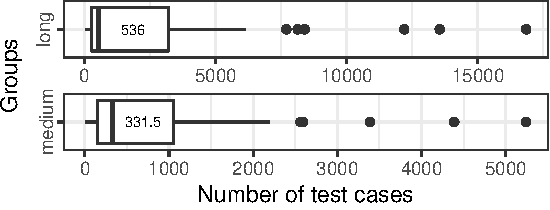
\includegraphics[width=.85\textwidth]{plots/boxplots-testcases.pdf}
    \caption{\label{fig:size-testsuites}Size of test suites.}
  \end{subfigure}
  ~
  \begin{subfigure}{0.3\textwidth}
    \centering
    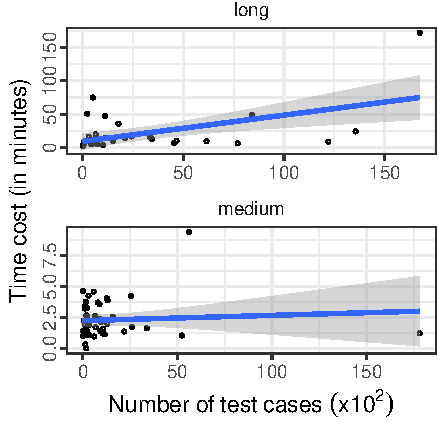
\includegraphics[width=.95\textwidth]{plots/scatter-testcost.pdf}
    \caption{\label{fig:scattercost}Size versus running time of
      test suites.}
  \end{subfigure}
  \caption{\label{fig:time-versus-size}Relating size and time.}%
\end{figure}

%\Mar{$\leftarrow$ show stats to indicate discrimination of
%  two distributions}

Figure~\ref{fig:time-distributions} showed that the average median
times were similar for \medg{} and \longg{}-running test suites.
Results indicate that the difference in overall running times of
projects in those groups was mainly justified by the number of test
cases as opposed to the individual costs of test cases.
Figure~\ref{fig:size-testsuites} shows the difference in the
distribution of test suite sizes across groups.  This figure indicates
that long projects, albeit having a wider inter-quartile range (middle
50\% projects in this group are less predictable), have a higher
median and much higher average number of test cases.  Furthermore, we
noted a strong positive correlation between running time and number of
test on projects in the \longg{} group.  Considering the \medg{}
group, the correlation between these two variables was weak.
Figure~\ref{fig:scattercost} illustrates this correlation.

%% however, weak in
%% the suggesting that saving time in this group with test suite
%% parallelization may be more challenging as relatively fewer tests
%% dominate overall execution time.  Figure~\ref{fig:scattercost} shows
%% these results.

%% This 
%% indication that it is more beneficial to parallelize long projects as
%% cost is spread across many

\vspace{1ex}
\begin{center}
\fbox{
\begin{minipage}{8cm}
    \textit{Answering \numRQFeasibilityTwo{}:}~\emph{Overall, results indicate that
    projects with a very small number of tests monopolizing end-to-end
    execution time were rare.}
\end{minipage}
}
\end{center}
\vspace{1ex}

%% We are interested to know whether
%% most of the execution cost of a subject is dominated by a small subset
%% of test cases or if the cost is nearly equally distributed. 

%% We also evaluated the dispersion of time distributions (one
%% distribution per project) to answer research question \numRQFeasibilityTwo{}.  To
%% measure dispersion \emph{across} projects we used Relative Standard
%% Deviation (RSD)~\cite{everitt-book-stats-2010}.  Note that, if we were
%% to analyze each project in isolation, the standard deviation of a
%% distribution ($\sigma$) would suffice to quantify how dispersed the
%% (time) distribution is.  However, in our case, we would like to be
%% able to compare and summarize dispersion across projects.  The RSD,
%% which is obtained dividing the standard deviation by the mean ($\mu$)
%% of a distribution, provides such normalization effect.  This metric
%% provides a lower bound (zero) but not an upper bound (somewhere close
%% to 1).  The smaller (larger) the value of RSD the more (less) uniform
%% the distribution is.  Consequently, the lower the value of RSD the
%% more parallelizable a test suite should be.

%% \begin{figure}[h!]
%%   \centering
%%   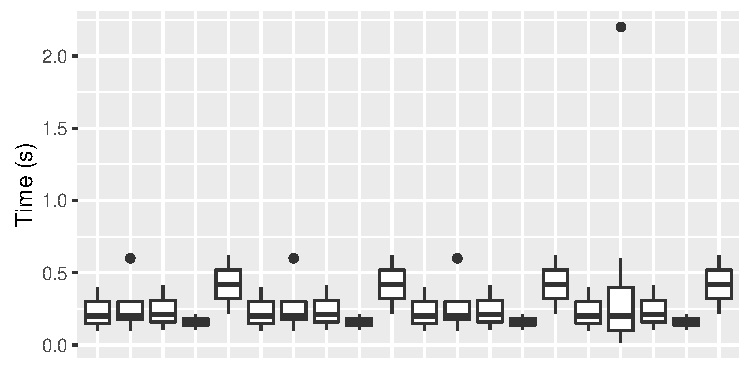
\includegraphics[width=0.5\textwidth]{R/testcost.pdf}  
%%   \caption{\label{fig:relativesd}Distribution of RSD ($\sigma/\mu$)
%%     across projects.}
%% \end{figure}

%% Figure~\ref{fig:relativesd} shows the distribution of RSD across
%% medium and long-running projects.  Results show that the distribution
%% is skewed to the right indicating that test costs are relatively well
%% distributed in most costly projects we analyzed \Fix{$\leftarrow$
%%   confirm}.

%% analyzed the execution time
%% for the \numMedLong{} projects from the \longg{} and \medg{} groups
%% (see Section~\ref{sec:rqA}).
%% For each subject we calculated the
%% relative standard deviation of the test cases: we collected the
%% elapsed time of each individual test, calculated the standard
%% deviation, and divided by the mean. \Jbc{I need to clarify the
%%   relationship "well/bad-balanced" regression test and relative
%%   standard deviation}

%% Results indicated that \Fix{...elaborate...}. \Jbc{We may identify
%% different groups of subjects}\Fix{TODO: collect data + compute the
%% statistic, create a scatter plot to identify groups of subjects}

%% Regression tests that are well distributed may benefit from
%% parallelism since more tests executes at the same time while the
%% opposite scenario may require a different approach. In the later
%% scenario, executing tests in parallel may have insignificant impact
%% since a small subset of test cases dominates the execution.}


\subsection{Adoption}
\label{sec:rqC}
\label{sec:rqE}

The dimension adoption focuses on the usage of parallelism in
open-source projects.  It evaluates (\numRQAdoptionOne) how often open-source
projects use parallelization schemes and (\numRQAdoptionTwo) how developers
involved in costly projects, not using parallelization, perceive this
technology.

\begin{itemize}
    \item \numRQAdoptionOne. \textbf{\RQAdoptionOne{}}
\end{itemize}

To answer \numRQAdoptionOne{}, we selected all projects from the \medg{} and
\longg{} groups, \ie, projects that ran in at least one minute.  This
set includes \numMedLong{} projects (see Section~\ref{sec:rqA}).  We
looked for dynamic and static manifestations of parallelism.

%% The
%% following section report results for each of these cases.

\vspace{1ex}
\subsubsection{Dynamic checking}
\label{sec:rqC-1}

To find dynamic evidence of parallelism, we ran the test suites from
our set of \numMedLong{} projects to output all key-value pairs of
Maven parameters.  To that end, we used the option~\CodeIn{-X} to
produce debug output and the option~\CodeIn{-DskipTests} to skip
execution of tests.  We skipped execution of tests as we observed from
sampling that only bootstrapping the Maven process suffices to infer
which parallel configuration modes it will use to actually run the
tests.  It is also important to point that we used the default
configurations specified in the project.  We inferred parallel
configurations by searching for certain configuration parameters in
log files. According to Maven's
documentation~\cite{maven-surefire-plugin}, a parallel configuration
depends either on (1) the parameter \CodeIn{parallel} to define the
parallelism mode within a JVM followed by the parameter
\CodeIn{threadCount} or (2) the parameter
\CodeIn{forkCount}\footnote{This parameter is named \CodeIn{forkMode}
  in old versions of Maven Surefire} to define the number of forked
JVMs.  As such, we captured, for each project, all related key-value
pairs of Maven parameters and mapped those pairs to one of the
possible parallelization modes.  For instance, if a given project
contains a module with the parameter
\CodeIn{<forkCount>1C</forkCount>}, the possible classifications are
\ForkSeq{} or \ForkParMeth{}, depending on the presence and the value
of the parameter \CodeIn{parallel}.  If the parameter
\CodeIn{parallel} is set to \CodeIn{methods} the detected mode will be
\ForkParMeth{}.  Large projects may contain several test suites
distributed on different Maven modules potentially using different
configurations.  For those cases, we collected the Maven output from
each module discarding duplicates as to avoid inflating counts for
configuration modes that appear in several modules of the same
project. For instance, if a project contains two modules using the
same configuration, we counted only one occurrence.


\begin{wrapfigure}{r}[0pt]{0pt}%0.525\linewidth
  \footnotesize
  %  \small
  \centering
  \setlength{\tabcolsep}{2.5pt}
%    \resizebox{.48\textwidth}{!}{%
    \begin{tabular}{lrr}
        \toprule
        \emph{Subject} & \emph{\# of modules} & \emph{Mode}\\%
        \midrule%
        \Comment{BounceStorage }Chaos\Comment{ HTTP Proxy} & 1/1 &  \ParClassSeqMeth{}\\%
        \Comment{Apache }Flink & 74/74 & \ForkSeq{} \\%        
        \Comment{JenkinsCI }Gerrit\Comment{ Trigger Plugin} & 1/1 & \ForkSeq{}\\%
        \Comment{Spotify }Helios & 8/8 & \ForkSeq{}\\%
        Javaslang & 3/3 & \ParClassParMeth{}\\%
        Jcabi\Comment{ Github} & 1/1 & \ParClassParMeth{}\\%        
        \Comment{Hazelcast }Jet & 7/14 & \ForkSeq{}\\%
        \Comment{Apache Logging }Log4J2 & 25/31 & \ForkSeq{}\\%
        \Comment{Jankotek }MapDB & 1/2 & \ParClassParMeth{}\\%        
        \bottomrule%
    \end{tabular}
    \caption{Subjects with parallel test execution enabled by
    default.}
    \label{tab:freqmodes-dynamic}
\end{wrapfigure}
Figure~\ref{tab:freqmodes-dynamic} shows the projects we idendified
where parallelism is enabled by default in Maven.  Column
``\emph{Subject}'' indicates the name of the project, column
``\emph{\# of modules}'' indicates the fraction of modules containing
tests that use the configuration of parallelism mentioned in column
``\emph{Mode}''.  We note that, considering these projects, the
modules that do not use the configuration cited use the sequential
configuration \Seq{}.  For example, six modules (=31-25) from Log4J2
use sequential configuration.

It came as a surprise the observation that
no project used distinct configurations in their modules. Considering
our set of \numMedLong{} projects, we found that only
\textbf{\numProjectsPar{}} of those projects had parallelism enabled
by default, with only configurations \ParClassSeqMeth{},
\ParClassParMeth{}, and \ForkSeq{} being used.  Configurations
\ParClassParMeth{} and \ForkSeq{} were the most popular among these
cases.  Note that these results under-approximate real usage of
parallelism as we used default parameters in our scripts to spawn the
Maven process.  That decision could prevent execution of particular
test modules.
%\begin{figure}[h!]
%    \centering
%    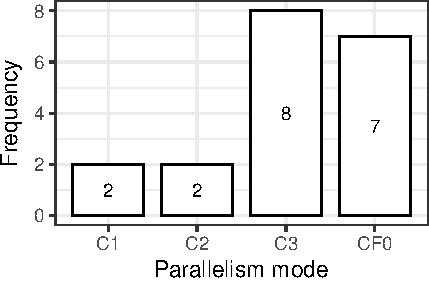
\includegraphics[width=0.32\textwidth]{plots/barplot-modes-dynamic.pdf}
%    \caption{\label{fig:freqmodes-dynamic}\Fix{fix
%    caption}Distribution of parallel modes identified dynamically in a
%    subset of \numProjectsPar{} projects.  A project may have support
%    to more than one parallel mode. Also, a project may run only a
%    subset tests in parallel by default.}
%\end{figure}

%% Recall that some projects can use parallel execution that is only
%% activated when developers pass certain parameters to the build
%% process. For instance, it is possible to create in Maven multiple
%% configurations in the same build file and select dynamically which one
%% should be used.  

\subsubsection{Static checking}
\label{sec:rqC-2}
Given the inherent limitation of dynamic monitoring to find evidence
of parallelism, we also looked for indication of parallelism in build
files\Comment{ in the same sample set of \numMedLong{} projects}.  We
parsed all \emph{pom.xml} files under the project's directory and used
the same approach as in our previous analysis to classify
configurations.  We noticed initially that our approach was unable to
infer the configuration mode for cases where the decision depends on
the input (\eg,
\CodeIn{<parallel>\$\{parallel.type\}</parallel>}). For these
projects, the tester needs to provide additional parameters in the
command line to enable parallelization (\eg, \CodeIn{mvn test
  -Dparallel.type=classesAndMethods}). To handle those case, we
considered all possible values for the parameter (in this case,
\CodeIn{\$\{parallel.type\}}).  It is also important to note that this
approach is not immune to false negatives, which can ocurr when
\emph{pom.xml} files are encapsulated in jar files or downloaded from
the network.  Consequently, this static checking is complementary to
the dynamic checking, previously presented.

Overall, we found, using this methodology, ten projects that use
parallelism.  Compared to the set of projects listed in
Figure~\ref{tab:speedup}, we found two new projects, namely:
\CodeIn{Google Cloud\Comment{ Platform} DataflowJavaSDK} (using
configuration C3) and \CodeIn{Mapstruct} (using configuration
\ForkSeq{}).  Curiously, we also found that project \CodeIn{Jcabi} was
not detected using this methodology.  That happened because this
project loads its \emph{pom.xml} file from a jar file that we did not
check.  Considering the static and dynamic methods together, we found
a total of 11 distinct projects using parallelism, corresponding to
the union of the two subject sets.

\vspace{1ex}
\begin{center}
\fbox{
  \begin{minipage}{8cm}
      \textit{Answering \numRQAdoptionOne{}:}~\emph{Results indicate that test
        suite parallelization is underused.  Overall, only
        \percentParallel{} of costly projects (11 out of \numMedLong)
        use parallelism.}
  \end{minipage}
}
\end{center}
\vspace{1ex}

%False positive can happen because of comments, for instance.  
%To eliminate the cases of false positives and also to categorize 
%true positive cases, we complemented the initial mining step with a 
%manual inspection of files.
%% settings); the second step (inspection) consists in a manual
%% inspection to confirm the presence of parallelism settings in the
%% build file and classify them according to the parallelism level.
%% Figure \Fix{removed} describes the discovery step: we list the paths
%% of all build files and filter only the files that contain any of the

%% Figure~\ref{tab:inspection-table} summarizes our results.
%% \Fix{The first column indicates the group of projects according to
%% their time cost.  The second column indicates the number of build
%% files per group.  The last column indicates the ratio of projects with
%% parallelization settings.  From the \numMedLong{} subjects, we found
%% \pomMedLong{} \pomf{} files.  The \numPomMatched{} configurations are
%% distributed across \numProjectsPar{} projects from our sample.}

%% % \emph{From these results we found that $\sim$51\% of medium and
%% % long-running projects do not use parallel features to run test
%% % suites.}\Mar{please make it consistent with research
%% % question}\Mar{explain this is over(under)-estimated...}
%% \begin{figure}[ht!]
%%     \centering
%%     \resizebox{.48\textwidth}{!}{%
%%     \begin{tabular}{llcl}
%%         \toprule
%%         Group & Subject & \# of modules & Mode\\%
%%         \midrule%
%%         Long   &JenkinsCI Gerrit Trigger Plugin& 1 & \ForkSeq\\%
%%         Medium &Bouncestorage Chaos Http Proxy & 1 & C2\\%
%%         Medium &Javaslang & 1 & C3\\%
%%         Medium &Apache Flink & 1 &\ForkSeq\\%
%%         Medium &Apache Logging Log4J2 & 3 & \ForkSeq{}\\%
%%         Medium &Google Cloud Platform DataflowJavaSDK & 1 & C3\\%
%%         Medium &Hazelcast Jet & 1 & \ForkSeq\\%
%%         Medium &Jankotek MapDB & 1 & C3\\%
%%         Medium &Mapstruct & 1 & \ForkSeq\\%
%%         Medium &Spotify Helios & 3 & \ForkSeq\\%
%%         \bottomrule%
%%     \end{tabular}}
%%     \caption{Subjects with parallelization configurations in build files.}
%%     \label{tab:inspection-table}
%% \end{figure}

%% \begin{figure}[ht!]
%%     \centering
%%     \begin{tabular*}{0.48\textwidth}{@{\extracolsep{\fill}}ccc}
%%         \toprule
%%         \multirow{2}{*}{Group} %1st row, 1st cell
%%             & \multirow{2}{*}{\# \pomf{}}
%% 	    & \# \pomf{} matched\\
%%         % 2nd row - empty cell
%%             & % empty cell
%%             & / total\\%
%%         \midrule%
%% 	Long   & \numPomLong{} & 4 / \numLong{}\\%
%% 	Medium & \numPomMed{} & 6 / \numMed{}\\%
%%         \midrule%
%%         Total % last row, first cell
%%             & \pomMedLong{}
%%             & \numProjectsPar{} / \numMedLong{}\\%
%%         \bottomrule%
%%     \end{tabular*}
%%     \caption{Presence of parallelization settings in build files: the
%%     first column indicates the group of projects according to their
%%     time cost; the second column is the subset of files with parallelization
%%     keywords; the last column indicates the ratio of projects with
%%     parallelism support.}
%%     \label{tab:inspection-table} 
%% \end{figure}
%% \Jbc{rework this... $\rightarrow$} From the \numProjectsPar{} projects
%% identified above, we investigated further the \numPomMatched{}
%% build files with parallel settings.  We analyzed the support and
%% distribution of parallel modes from this subset of projects. To
%% calculate the distribution of parallel modes, we considered only the
%% presence of the mode in at least one of the project settings.  Recall
%% that a build file may contain more than one parallel setting and a
%% project may contain several sub-modules with build files.  In case the
%% value of a parallel option is resolved dynamically (\eg, via
%% command-line argument or system variable) we compute all modes related
%% to the option. For instance, depending on the value, the
%% \CodeIn{parallel} option can be \Seq{} (\CodeIn{none}),
%% \ParClassSeqMeth{} (\CodeIn{classes}), \SeqClassParMeth{},
%% (\CodeIn{methods}), and \ParClassParMeth{} (\CodeIn{all}).
%% Figure~\Fix{fig:freqmodes-static} summarizes our findings.
%% \Fix{Missing conclusion: Fork the most used configuration}
%% \begin{figure}[h!]
%%     \centering
%%     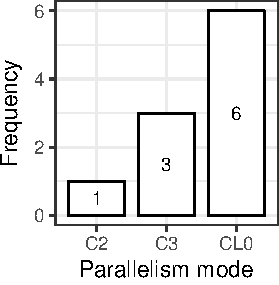
\includegraphics[width=0.32\textwidth]{plots/barplot-modes-static.pdf}
%% 	\caption{\label{fig:freqmodes-static}\Luis{This is wrong, it
%% 	should be \textbf{CF0} instead of \textbf{CL0}}Distribution of parallel modes
%%     identified statically in a subset of \numProjectsPar{} projects.
%%     A project may have support to more than one parallel mode.}
%% \end{figure}


\begin{itemize}
	\item \numRQAdoptionTwo{}. \textbf{\RQAdoptionTwo{}}
\end{itemize}

To answer this research question we surveyed developers involved in a
selection of projects from our benchmark with time-consuming test
suites.  The goal of the survey is to better comprehend developer's
attitude towards the use of parallelism as a mechanism to speedup
regression testing.  We surveyed developers from a total of
\emailsProjects{} projects.  From the initial list of \numMedLong{}
project, we discarded 11 projects that we knew a priori used
parallelization, and \discartedProjects{} projects that we could not find
developer's emails from commit logs.  From this list of projects, we
mined potential participants for our study.  More precisely, we
searched for developer's name and email from the last 20 commits to
the corresponding project repository.  Using this approach, we
identified a total of \emailsSent{} eligible participants.  Finally,
we sent plain-text e-mails, containing the survey, to those developers.  In
total, \emailsAnswered{} developers replied but we discarded
\emailsFalseAnswers{} replies with subjective answers.  Considering
projects covered by the answers, a total of \emailsProjectsAnswered{}
projects (\percEmailsProjectsAnswered{} of the total) were represented
in those replies.  Note that multiple developers on each project
received emails.  We sent the following set of questions to
developers:

\begin{enumerate}
\item How long does it take for tests to run in your environment? Can
  you briefly define your setup?
\item Do you confirm that your regression test suite does *not* run in parallel?
\item\label{questionThree} Select a reason for not using parallelization:
  \begin{enumerate}[label=\alph*)]
  \item I did not know it was possible
  \item I was concerned with concurrency issues
  \item I use a continuous integration server
  \item Some other reason. Please elaborate.
  \end{enumerate}
\end{enumerate}

%% \begin{enumerate}
%% 	\item How long does it take for test to run in your
%%		environment?
%%	\item Can you briefly define your setup?
%%	\item Do you confirm that your project does not run in
%%		parallel?
%%	\item Select a reason for not using paralellization:
%%		\begin{enumarate}
%%			\item I did not know it was possible;
%%			\item I was concerned with concurrency issues;
%%			\item I use a continuous integration server;
%%			\item Some other reason.
%%		\end{enumerate}
%% \end{enumerate}
%% One of the goals of the first questions is to identify potential
%% discrepancies between our experimental environment and the environment
%% of developers.  Overall, we found that \Fix{...}

Considering question 1, we confirmed that execution time was
compatible with the results we reported in Section~\ref{sec:rqA}.
Furthermore, \emailsCI{} of the participants indicated the use of
Continuous Integration (CI) to run tests, with \emailsDistributed{} of
these participants reporting that test suites are modularized and
those modules are tested independetly in CI servers through different
parameters.  Those participants argumented that such practice helps to
reduce time to observe test failures, which is the goal of speeding up
regression testing.  A total of \emailsLocal{} participants answered
that they do run tests in their local machines.  Note, however, that
CI does not preclude low-level parallelization.  For example,
installations of open-source CI tools (\eg{}, Jenkins~\cite{jenkins})
in dedicated servers would benefit from running tests faster through
low-level test suite parallelization.

% \emailsNotDescribed{} developers did not described their environment.

Considering question 2, the answers we collected indicated, to our
surprise, that six of the \emailsProjectsAnswered{} projects execute
tests in parallel.  This mismatch is justified by cases where neither
of our checks (static or dynamic) could detect presence of
parallelism.  A closer look at these projects revealed that one of
them contained a \emph{pom.xml} file encapsulated in a jar file
(similar case as reported in Section~\ref{sec:rqC-2}), in one of the
projects the particpant considered that distributed CI was a form of
parallelism, and in four projects the team preferred to implement
parallelization instead of using existing features from the testing
framework and the build system~---~in two projects the team
implemented concurrency control with custom JUnit test runners and in
two other projects the team implemented concurrency within test
methods.  Note that, considering these four extra cases (ignored two
distributed CI cases), the usage of parallelization increases from
\percentParallel{} to \percentParallelUpdated{}.  We do not consider
this change significant enough to modify our conclusion about
practical adoption of parallelization (\numRQAdoptionOne{}).

%% , one runs a manually created Thread to run some
%% tests, and the other runs in parallel by using Java 8 collection
%% streams, that allows the developers to iterate over a list in
%% parallel.

%% did not confirmed, however,
%% the developers confirmed the need of an extra parameter at the command
%% line to execute in parallel.

Considering question 3, the distribution of answers was as follows.  A
total of \emailsA{} of the \emailsProjectsAnswered{} developers who
answered the survey did not know that parallelism was available in
Maven (option ``a''), \emailsB{} of developers mentioned that they did
not use parallelism concerned with possible concurrency issues (option
``b''), \emailsD{} of developers mentioned that continuous integration
services sufficed to provide timely feedback while running only smoke
\begin{wrapfigure}{r}[0pt]{0pt}%0.525\linewidth
    \centering
    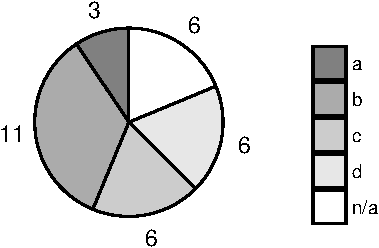
\includegraphics[width=.18\textwidth]{plots/survey.pdf}
    \caption{\label{fig:rq5-answers}Summary of developer's answers to
      survey question~\ref{questionThree}.}
\end{wrapfigure}
tests (\ie{}, short-running tests) locally (option ``c'')\Comment{here
  I want to say that they use it for something like "non-blocking
  testing" while developing in a local machine}, and \emailsD{} of
developers who provided an alternative answer (option ``d'') mentioned
that using parallelism was not worth the effort of preparing the test
suites to take advantage of available processing power.  A total of
\emailsNA{} of participants did not answer the last question of the
survey.  The pie chart in Figure~\ref{fig:rq5-answers} 
summarizes the distribution of answers.

\begin{center}
\fbox{
	\begin{minipage}{8cm}
	  \textit{Answering \numRQAdoptionTwo{}:}~\emph{Results suggest that dealing
       with concurrency issues (\ie{}, the extra work to organize test
       suite to safely explore concurrency) was the principal reason
       for developers not investing in parallelism.  Other reasons
       included availability of continuous integration services and
       unfamiliarity with the technology.}
	\end{minipage}
}
\end{center}

\subsection{Speedups}
\label{sec:rqD}

\begin{itemize}
    \item \numRQSpeedupOne{}. \textbf{\RQSpeedupOne}
\end{itemize}

To answer \numRQSpeedupOne{}, we considered the \numProjectsPar{}
subjects from our benchmark that use parallelization \emph{by default}
(see Figure~\ref{tab:freqmodes-dynamic}).  We compared running times
with parallelization~---~configured by project owners~---~and without
parallelization.

%% In those projects, parallelization is active without
%% passing any extra parameters.  Section~\ref{sec:rqC-1} describes in
%% detail the methodology we used to find these subjects.
%and
%Section~\ref{seq:rq6-tradeoffs}, we verified that both
%% executions produce the same outcome to eliminate noise from failing
%% tests.  To compute the speedup, we divide the time obtained in the
%% sequential execution by the time obtained from the default execution.
%% For instance, if a project runs the tests sequentially in $10m$ and
%% the same execution runs in $5m$ with parallelization enabled (default
%% execution), the speedup is two.

Figure~\ref{tab:speedup} summarizes results.  Lines are sorted by
project names.  Columns ``\emph{Group}'' and
``\emph{Name}'' indicate, respectively, the group and the name of the
subject.  Column ``$T_s$'' shows sequential execution time and column
``$T_p$'' shows parallel execution time. Column ``$T_s/T_p$'' shows
speedup or slowdown.  As usual, a ratio above 1x denotes speedup
and a ratio below 1x denotes slowdown.

\begin{figure}[h!]
\centering
\resizebox{.41\textwidth}{!}{%
  \scriptsize
\begin{tabular}{llrrr}
\toprule
\emph{Group} & \emph{Subject} & \multicolumn{1}{c}{$T_s$} & \multicolumn{1}{c}{$T_p$} & $T_s/T_p$ \\%
\midrule%
Medium & \Comment{BounceStorage }Chaos\Comment{ HTTP Proxy} & 1.51m & 1.47m & 
    \cellcolor{lightgray}1.01x\\%
Medium &\Comment{ Apache }Flink& 11.79m & 2.57m & 4.59x\\%
Long &\Comment{ Jenkins CI }Gerrit\Comment{ Plugin} & 51.19m & 40.31m &  1.26x\\%
Medium &\Comment{ Spotify }Helios& 4.46m & 1.63m & 2.73x\\%  
Medium &Javaslang& 2.18m & 1.82m & 1.19x\\%
Medium &Jcabi\Comment{ GitHub} & 2.76m & 0.30m &
    \cellcolor{lightgray}9.2x\\%
Medium &\Comment{ Hazelcast }Jet& 8.26m & 3.67m & 2.25x\\%
Long &\Comment{ Apache }Log4J2& 8.24m & 8.21m & \cellcolor{lightgray}1.00x\\%
Long &\Comment{ Jankotek }MapDB& 10.06m & 8.58m & 1.17x\\%
\midrule
\textbf{average} &  &  &  & \avgSpeedup{}x\\
\bottomrule%
\end{tabular}}
\caption{\label{tab:speedup}Speedup (or slowdown) of parallel
  execution ($T_p$) over sequential execution ($T_s$).  Default
  parallel configuration of Maven is used.  Highest slowdown/speedup
  appears in gray color.}
\end{figure}

Results indicate that, on average, parallel execution was
\avgSpeedup{} times faster compared to sequential execution.  Three
cases worth special attention: \CodeIn{Chaos}, \CodeIn{Jcabi} and
\CodeIn{Log4J2}.  No significant speedup was observed in
\CodeIn{Chaos}, a project with only three test classes, of which one
monopolizes the bulk of test execution time.  This project uses
configuration \ParClassSeqMeth{}, which runs test classes in parallel
and test methods, declared in each class, sequentially.  Consequently,
speedup cannot be obtained as the cost of the single expensive test
class cannot be broken down with the selected configuration.  Although
project \CodeIn{Jcabi} also uses configuration \ParClassSeqMeth{},
results obtained are very different compared to \CodeIn{Chaos}.  The
speedup observed in \CodeIn{Jcabi} was the highest amongst all
projects.  This project contains test classes with a small number of
test methods and several methods in those classes are time-consuming.
As result, the CPUs available for testing are kept occupied for the
most part during test execution.  Finally, we note that parallel
execution in \CodeIn{Log4J2} was innefective.  We found that Maven
invokes several test modules in this project but the test modules that
dominate execution time run sequentially by default.

%% The third, runs parallel configuration in
%% \Fix{80\%} of the project modules, however, the test time is dominated
%% by one of the sequentially running modules.  \Luis{$\leftarrow$ rework
%%   this} \Fix{falar sobre o resultado geral dos speedups - elaborar
%%   menor e maior speedup... acho que so vale a pena discutir quando
%%   tiver conviccao dos 2 casos}

\begin{center}
\fbox{
  \begin{minipage}{8cm}
    \textit{Answering \numRQSpeedupOne{}:}~\emph{Considering the
      machine setup we used, the average speedup observed with default
      configurations of parallelization was \avgSpeedup{}x.}
  \end{minipage}
}
\end{center}

\begin{itemize}
    \item \numRQSpeedupTwo{}. \textbf{\RQSpeedupTwo}
\end{itemize}

\newcommand{\subjectScalability}{MapDB}

This experiment evaluates the impact of making available to the build
system a growing number of CPUs for testing.  For that reason, we used
a machine with more cores compared to the one described in
Section~\ref{sec:setup}.  We used a Xeon E5-2660v2 (2.20GHz) Intel
processor machine with 80 virtual CPUs (40 cores with two native
threads each) and 256GB of memory, running Ubuntu 14.04 LTS Trusty
Tarr (64-bit version). This experiment uses configuration \ForkSeq{}
\begin{wrapfigure}{r}[0pt]{0pt}%0.525\linewidth
    \centering
    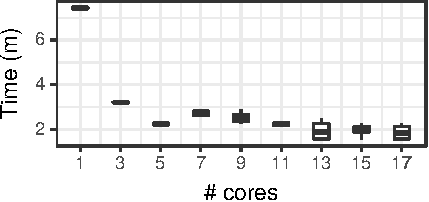
\includegraphics[width=.2\textwidth]{R/scalability/scalability.pdf}
    \caption{\label{fig:scalability}Scalability.}
\end{wrapfigure}
as the goal is to evaluate the impact on runtime of spawning a growing number of
JVMs in different CPUs.  Furthremore, we selected subject
\subjectScalability{} as it represents the case of a long-running test
suite (see Figure~\ref{tab:speedup}) with test cases distributed
across many test classes (194 test classes for \subjectScalability{}).
Note that a test class is the smallest unit that can be used to spawn
a test job on a JVM and that we have no control over which test
classes will be assigned to which JVM that the build system forks.

Figure~\ref{fig:scalability} shows the reduction of running times as
more CPUs contribute to the execution.  \Fix{elaborate...}

\begin{center}
\fbox{
  \begin{minipage}{8cm}
    \textit{Answering \numRQSpeedupTwo{}:}~\emph{...}
  \end{minipage}
}
\end{center}

\subsection{Issues}
\label{sec:rq6-tradeoffs}

This dimension assesses the impact of using distinct parallel
configurations on test flakiness (negative impact) and speedup
(positive impact).  Furthermore, note that Section~\ref{sec:rqD}
evaluated speedup in isolation, focused on projects configured to use
parallelism by default.

\begin{itemize}
    \item \numRQIssuesOne{}. \textbf{\RQIssuesOne{}}
\end{itemize}


%% The intuition is that efficiency and flakiness are inversely
%% proportional in some cases: if too many tests depends on the state of
%% a single external resource, several tests are likely to fail as the
%% degree of concurrency increases by exploiting maximum CPU usage.

%% Table header macros
% $\Uparrow_\text{speed}$
\newcommand{\subcolA}{$\text{speedup}$}
\newcommand{\subcolB}{$\%_\text{fail}$}
\newcommand{\colheader}[1]{\multicolumn{2}{c}{\emph{#1}}}
\newcommand{\blankentry}{\entry{-}{-}}
\newcommand{\subcol}{\subcolA{} & \subcolB{}}
\newcommand{\entry}[2]{#1 & #2}

\begin{figure*}[t]  
\centering
\small
\setlength{\tabcolsep}{3pt}
\begin{tabular}{l|rr|rr|rr|rr|rr|rr}
\toprule
\multirow{2}{*}{\emph{Subject (module)}} & \multicolumn{2}{c|}{\emph{\Seq}} &
    \colheader{\SeqClassParMeth} & \colheader{\ParClassSeqMeth} &
    \colheader{\ParClassParMeth} & \colheader{\ForkSeq} &
    \colheader{\ForkParMeth} \\ %\cline{2-12}
    & $T$ & $\mathit{N}$ & \subcol{} & \subcol{} & \subcol{} & \subcol{}
    & \subcol{}\\%
\midrule%
AWS SDK Java (\CodeIn{core})  & \entry{3.7m}{847}  & \entry{1.95x}{2.24\%} & \entry{2.47x}{2.77\%} & \entry{3.70x}{4.01\%} & \entry{}{} & \entry{}{}\\%

Facebook Linkbench    & \entry{4.3m}{98}  & \entry{1.00x}{0\%} & \entry{1.65x}{1.02\%} & \entry{1.59x}{1.02\%} & \entry{}{} & \entry{}{}\\%

GoogleCloud Dataflow Java (\CodeIn{sdk}) & \entry{1.6m}{3,345}  & \entry{1.23x}{1.67\%} & \entry{2.67x}{1.05\%} & \entry{0.80x}{5.35\%} & \entry{}{} & \entry{}{}\\%

Javaslang (\CodeIn{core})     & \entry{1.1m}{17,513}  & \entry{1.38x}{0\%} & \entry{1.83x}{0\%} & \entry{1.38x}{0\%} & \entry{}{} & \entry{}{}\\ 
JCabi Github                  & \entry{2.6m}{634} & \entry{2.10x}{0\%} & \entry{17.70x}{0\%} & \entry{28.80x}{0\%} & \entry{}{} & \entry{}{} \\
JCTools (\CodeIn{core})       & \entry{3.6m}{690}  & \entry{4.50x}{0\%} & \entry{3.60x}{0\%} & \entry{18.00x}{0\%} & \entry{}{} & \entry{}{}\\%
MapDB  & \entry{8.2m}{5,324}  & \entry{1.52x}{0\%} & \entry{2.73x}{0\%} & \entry{4.82x}{0.05\%}   & \entry{}{} & \entry{}{}\\%
Moquette                      & \entry{3.7m}{169} & \entry{4.62x}{65.64\%} & \entry{3.36x}{32.92\%} & \entry{12.33x}{77.78\%} & \entry{}{} & \entry{}{} \\
RipMe                         & \entry{1.1m}{54}  & \entry{0.94x}{0\%} & \entry{1.63x}{0\%} & \entry{1.63x}{0\%} & \entry{1.37x}{0\%} & \entry{1.42x}{0\%}\\
Stripe Java     & \entry{4.3m}{302}  & \entry{4.78x}{6.31\%} & \entry{3.31x}{7.31\%} & \entry{21.50x}{14.95\%} & \entry{}{} & \entry{}{}\\%





\midrule

\textbf{Average}   & \entry{-}{-} & \entry{-}{-} & \entry{-}{-} & \entry{-}{-}
& \entry{-}{-} & \entry{-}{-} \\%


%%  & \entry{x.xm}{0}  & \entry{}{\%} & \entry{}{\%} & \entry{}{\%} & \entry{}{} & \entry{}{}\\%
%%OpenMRS Core (\CodeIn{api})  & \entry{15.4m}{3436} & \blankentry{}        & \blankentry{}        & \blankentry{} & \entry{1.5x}{0\%} & \entry{1.7x}{0}\\%
%%Apache Flume (\CodeIn{core}) &  \entry{7.7m}{392}  & \blankentry{}        & \blankentry{}        & \blankentry{}       & \entry{0.9x}{0\%} & \blankentry{} \\%
%%Facebook Archive Linkbench   &  \entry{4.5m}{98}   & \entry{1.0x}{0.2\%}  & \entry{1.6x}{1.2\%}       & \entry{1.0x}{0\%}  & \entry{1.7x}{0.5\%}  & \entry{1.7x}{0.2\%}\\%
%%AWS SDK Java (\CodeIn{core}) &  \entry{3.8m}{847}  & \multicolumn{6}{c}{\Fix{requires investigation}} & \entry{2.2x}{0.1\%} & \entry{3.2x}{2.0\%}\\%

%% OpenMRS Core (\CodeIn{api})  & \entry{15.4m}{3436} & \blankentry{}        & \blankentry{}        & \blankentry{} & \entry{1.5x}{0\%} & \entry{1.7x}{0}\\%
%% Jankotek MapDB               &  \entry{9.9m}{5218} & \multicolumn{6}{c}{\cellcolor{lightgray}\emph{JVM Crash}} & \entry{1.5x}{0\%} & \entry{1.7x}{0\%}\\%
%% Apache Flume (\CodeIn{core}) &  \entry{7.7m}{392}  & \blankentry{}        & \blankentry{}        & \blankentry{}       & \entry{0.9x}{0\%} & \blankentry{} \\%
%% Apache Giraph (\CodeIn{core})&  \entry{7.2m}{236}  & \entry{2.1x}{5.1\%}  & \colheader{\cellcolor{lightgray}timeout}   & \entry{1.0x}{0\%} & \entry{1.0x}{0}\% & \colheader{\cellcolor{lightgray}JVM Crash}\\%
%% Facebook Archive Linkbench   &  \entry{4.5m}{98}   & \entry{1.0x}{0.2\%}  & \entry{1.6x}{1.2\%}       & \entry{1.0x}{0\%}  & \entry{1.7x}{0.5\%}  & \entry{1.7x}{0.2\%}\\%
%% Stripe Java                  &  \entry{4.2m}{302}  & \entry{4.2x}{5.2\%}  & \entry{3.5x}{5.7\%}       & \entry{4.2x}{6.3\%} & \entry{1.0x}{0.3\%} & \entry{4.2x}{5.7\%}\\%
%% AWS SDK Java (\CodeIn{core}) &  \entry{3.8m}{847}  & \multicolumn{6}{c}{\Fix{requires investigation}} & \entry{2.2x}{0.1\%} & \entry{3.2x}{2.0\%}\\%

%% Jenkins CI Github            & \entry{Xm}{Z}       & \entry{x}{\%}          & \entry{x}{\%} & \entry{x}{\%} & \entry{x}{\%} & \entry{x}{\%}\\%
%% Jenkins CI Docker Workflow   & \entry{Xm}{Z}       & \entry{x}{\%}          & \entry{x}{\%} & \entry{x}{\%} & \entry{x}{\%} & \entry{x}{\%}\\%
%% Hazelcast                    & \entry{Xm}{Z}       & \entry{x}{\%}          & \entry{x}{\%} & \entry{x}{\%} & \entry{x}{\%} & \entry{x}{\%}\\%

\bottomrule%
\end{tabular}
\caption{Speedup versus Flakiness (\subcolB). Configuration
  \emph{\Seq{}} denotes the comparison baseline, which runs tests
  sequentially.  Columns $T$ and $N$ indicate time and number of
  tests, respectively.  Other columns show speedup and percentage of
  failing tests in different configurations, compared to
  \emph{\Seq{}}.\Mar{Can you please add name of module for all subjects?}}
\label{tab:rq6-table}
\end{figure*}

To answer this research question, we conducted an experiment involving
the six parallel configurations from Section~\ref{sec:modes}  and the
top 10 long-running test modules from our sample set. The rationale
for this selection criteria was to maximize the chances of observing
speedup and flakiness, assuming that long-running tests also have many
tests. Indeed, we confirmed that test suites in these projects contain
at least 236 tests ($1,662.7$ in average). Also, we preferred to compare the
effect of a configuration over a single test module for projects with
multiple test modules.  Recall that large projects may contain several
test modules, and these modules may contain distinct characteristics
that could favor one configuration and not others; therefore, it would
be necessary to check each module individually for a fair comparison.
We are interested in understanding how efficiency (\ie, testing cost)
and flakiness (\ie, failing tests) are affected when we run a test
suite with different parallel configurations.  Recall that increased
resource contention obtained with parallelism can lead to concurrency
issues such as data races.  Flakiness and speedup are contradictory
forces that drive configuration selection.  We used as a \emph{control
group} (\ie, baseline) the sequential execution of each subject's
tests. Notice that for measuring flakiness, we have to consider only
tests that failed due to the concurrency in the parallel execution.
For that reason, we re-executed the tests in sequence ten times and
carefully verified that there are only passing tests in our baseline.
We considered ten as the number of re-executions based on the approach
used by Google reported in a previous work on test
flakiness~\cite{luo-etal-fse2014}.  To obtain parallel configurations,
we implemented a script that takes a subject and a configuration (\eg,
\ForkSeq{}) as inputs, and the script outputs the modified version of
the subject with the desired configuration. The workflow consists in
copying the project directory to a new directory, finding all existing
build files (\ie, \pomf{} files), and modifying all existing Maven
Surefire configurations with new values for the parameters
\CodeIn{parallel}, \CodeIn{forkCount}, and \CodeIn{threadCount} using
an XPath~\cite{xpath} library to manipulate XML documents. For
configurations with forked JVMs enabled (\ie, \ForkSeq{} and
\ForkParMeth{}), we changed the \CodeIn{forkCount} with the value
\CodeIn{1C} (\ie, one JVM per core).  To adjust the pool of threads
for parallelism within a JVM, we changed the parameter
\CodeIn{threadCount} with \Jbc{should we consider 2 as it is the
number of native threads per core OR 6 as it represents 3 Cores * 2
native threads?}.  To run the subjects and their respective variations
(\ie, the modified versions according to the parallelism
configuration), we used a similar approach as described in


Figure~\ref{fig:mvn-execution} except that we added a timeout of one
hour to run the tests. We used the \CodeIn{timeout}
command~\cite{timeout-cmd} to monitor the execution, and we configured
the command to dispatch a \emph{kill} signal if the test execution
exceeds the time limit. We imposed this time constraint to avoid
hanging indefinitely the experiment execution due to some thread
contention that may occur (\eg, deadlock). Finally, we saved each
execution log and XML test reports generated by Maven to collect the
execution time, the number of failing tests, and for reference to
analyze and diagnose outliers in our results. For efficiency, we
reported the speedup (\ie, $\Uparrow_\text{speed} = T_{\text{s}} /
T_{\text{p}}$) in average, and for flakiness, we reported the rate of
failing tests (\ie, $\mathit{\%_\text{fail} = failures / tests}$) in
average.  Figure~\ref{tab:rq6-table} summarizes the obtained results
ordered by the time cost (\ie, $T_\text{cost}$). \Fix{Remember to
explain efficiency cutoff, JVM crashes and timeout}

\Jbc{Lembrar que investigar o slowdown de Dataflow... os logs indicam que varios
dos testes que quebraram tentavam fazer uma autenticacao em algum servico.
Possivelmente o slowdown se deve ao tempo de resposta do servico quando
a autentiticao falha}

%% \begin{figure}[h!]
%% \centering
%% \resizebox{.48\textwidth}{!}{%
%% \begin{tabular}{lcrrrrr}
%% \toprule
%% \emph{Subject} & \emph{\# of tests} & \emph{\SeqClassParMeth{}} & \emph{\ParClassSeqMeth{}} & \emph{\ParClassParMeth{}} & \emph{\ForkSeq{}} & \emph{\ForkParMeth{}}\\%
%% \midrule%
%% Linkedin Pinot & 356 & - & - & - & - & -\\%
%% %% Jenkins CI Github Plugin & - & - & - & - & 0\% & -\\%
%% %% Kite SDK & - & - & - & - & - & -\\%
%% %% \Fix{!?} Apache Giraph & 327 & - & - & - & - & -\\%
%% %% OpenMRS Core & - & - & - & - & - & -\\%
%% %% Jenkins CI Docker Workflow Plugin & - & - & - & - & 0\% & -\\%
%% %% \Fix{Flaky} Apache Eagle & - & - & - & - & - & -\\%
%% %%Geotools & 7701 & - & - & - & - & -\\%
%% %%Kuromoji & 672 & - & - & - & - & -\\%
%% %%Atomix & 99 & - & - & - & - & -\\%
%% %%\Fix{Snazy OHC} & - & - & - & - & - & -\\%
%% %%\Fix{RoaringBitmap} & - & - & - & - & - & -\\%
%% \bottomrule%
%% \end{tabular}}
%% \caption{\Fix{Tabela de flakiness}}
%% \label{tab:rq6-flaky}
%% \end{figure}

\Fix{Elaborate results from efficiency}

\Fix{Elaborate results from flakiness}

\Fix{highlight special cases}

\Fix{Draw conclusions}

\begin{center}
\fbox{
\begin{minipage}{8cm}
\textit{Answering \numRQIssuesOne{}:~\emph{\Jbc{summarize findings...}}}
\end{minipage}
}
\end{center}

%%  LocalWords:  RQ occurence parallelization Tradeoffs API readme th
%%  LocalWords:  mvn clearcut escapeinside xleftmargin untestable LTS
%%  LocalWords:  framexleftmargin CPUs Tahr sysstat gh Vagrantfile
%%  LocalWords:  javadoc isolcpus JUnit's JUnitCore Gligoric boxplots
%%  LocalWords:  outliers apache uber chaperone facebookarchive
%%  LocalWords:  linkbench priori


We ran the test suite for each subject three times, reporting averaged
execution times in three ranges: tests that run within a minute
(\shortg{} group), tests that run in one to five minutes (\medg{}
group), and tests that run in five or more minutes (\longg{}
group). We followed a similar methodology to group projects by time as
Gligoric~\etal{}~\cite{gligoric-etal-issta2015} in their work on
regression test selection.\Comment{ and added the \medg{} group due to
  the variability of the time cost from subjects out of the \shortg{}
  group} Figure~\ref{fig:rq1-barplot} shows the number of projects in
each group.  As expected, \longg{} and \medg{} projects do not occur
as frequently as \shortg{} projects.  However, they do occur in
relatively high numbers.

Figure~\ref{fig:rq1-boxplot} shows cost distribution of test suites in
each group as boxplots.  Note that the y-ranges are different.  The
distribution associated with the \shortg{} group is the most
unbalanced (right skewed)\Comment{ with outliers closed to the \medg{}
  group}.  The test suites in this group ran in 15 or less seconds for
over 75\% of the cases.  Such scenarios constitute the majority of the
cases we analyzed.  Considering the groups \medg{} and \longg{},
however, we found many costly executions.  Nearly 75\% of the projects
from the \medg{} group take over 3.5 minutes to run and nearly 75\% of
the projects from the \longg{} group take $\sim$20 minutes to run.  We
found cases in the \longg{} group were execution takes over 50 minutes
to complete, as can be observed from the outliers (dots) in the plot.

%% the median from the
%% \medg{} group is nearly two minutes and most of the subjects run in
%% less than four minutes; most of the \longg{} group runs in less than
%% 25 minutes but has outliers that require more than 50 minutes to
%% execute.



\begin{figure}[ht]
    \centering
    \begin{subfigure}{0.182\textwidth}
        \centering
        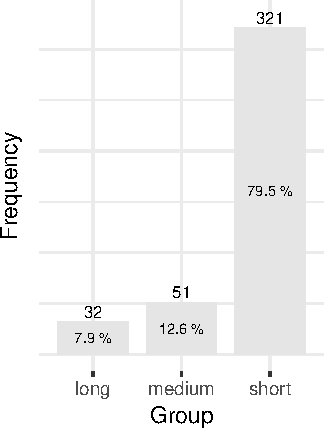
\includegraphics[width=\textwidth]{plots/barplot-timecost.pdf}
        \caption{\label{fig:rq1-barplot}}
    \end{subfigure}%
    ~
    \begin{subfigure}{0.25\textwidth}
        \centering
        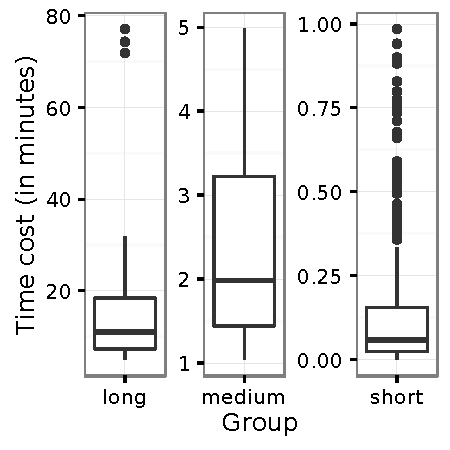
\includegraphics[width=\textwidth]{plots/boxplot-timecost.pdf}
        \caption{\label{fig:rq1-boxplot}}
    \end{subfigure}%
    \caption{(a) Subjects grouped by time cost ($t$): short run ($t <
    1m$), medium run ($1m \le t < 5m$), and long run ($5m \le t$); (b)
    Distribution of time cost by group.}
\end{figure}

%% Figure~\ref{fig:rq1-barplot} is a lower bound estimation of cost
%% because some tests may finish earlier than expected due to existing
%% test failures in the revision we downloaded.

It is important to note that we under-estimated cost in our
experiments for two main reasons.  First, some tests may finish
earlier than expected due to the observed test failures in some of the
revisions we downloaded.  From the \numSubjs{} testable projects,
\numSubjsPass{} successfully executed all tests and \numSubjsFail{}
reported some test failures.  Second, some projects may omit
long-running tests on their default execution. For instance, the
project \CodeIn{apache.maven-surefire} runs all unit tests in a few
seconds.  According to our criteria, this project is to be classified
as \shortg{} but a closer look reveals that only smoke tests are run
by default in this project.  Time-consuming integration and system
tests are only accessible via custom parameters, which we do not
handle in our experimental setup.  We enabled such parameters for this
specific project and observed that testing time goes to nearly 30
minutes.  For simplicity, we considered only the tests executed by
default.

\vspace{1ex}
\begin{center}
\fbox{
\begin{minipage}{8cm}
    \textit{Answering \numRQFeasibilityOne{}:}~\emph{We conclude that
      time-consuming test suites are relatively frequent in
      open-source projects.  We found that \percentMedLongRunning{} of
      the \numSubjs{} projects we analyzed (\ie{}, over 1 in every 5
      projects) take at least 3 minutes to run and
      \percentLongRunning{} take at least 5 minutes to run.\Comment{
        (\ie, \numMedLong{} projects from \medg{} and \longg{}).}}
\end{minipage}
}
\end{center}
\vspace{1ex}


\begin{itemize}
    \item \numRQFeasibilityTwo. \textbf{\RQFeasibilityTwo}
\end{itemize}

Section~\ref{sec:rqA} showed that medium and long-running projects are
not uncommon, accounting to nearly \percentMedLongRunning{} of the
\numSubjs{} projects we analyzed.  Research question \numRQFeasibilityTwo{}
measures the distribution of test costs in test suites as to estimate
(lack of) potential of obtaining speedups with parallelization.  In
the limit, if cost is dominated by a single test from a large test
suite, it is unlikely that parallelization will be beneficial as a
test method is the smallest working unit in test frameworks.

%% However, avoiding
%% frequent context switches is another factor to consider.  For example,
%% assuming there are at least two CPUs available for execution, cost can
%% be cut in half if two tests in a large test suite dominate execution
%% time and these tests are assigned to different CPUs.

%% It is therefore important to
%% speedup regressing testing in open-source projects.\Comment{not only
%%   to huge projects as those from Google~\cite{google-tap,google-ci}
%%   and Microsoft~\cite{prasad-shulte-ieee-microsoft-ci}.}



%% For the case
%% where cost is distributed more evenly across test cases, one expects
%% that speedups will be a function of the number of cores.
%% These contradictory forces, pushing number of tests and cost
%% of each test up and down, make prediction of effectiveness challenging.

\begin{figure}[h]
    \centering
    \begin{subfigure}{0.47\textwidth}
      \centering
      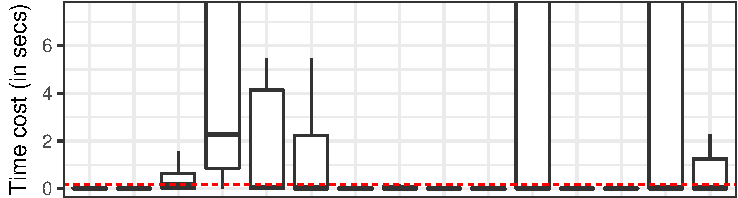
\includegraphics[width=\textwidth]{plots/testcost-long.pdf}
      \caption{\label{fig:longtcost}Long group.}
    \end{subfigure}\\
    \vspace{2ex}
    \begin{subfigure}{0.47\textwidth}
      \centering
      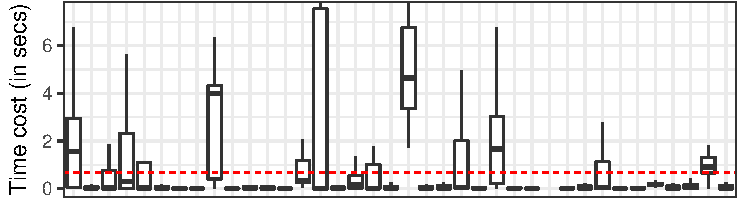
\includegraphics[width=\textwidth]{plots/testcost-medium.pdf}
      \caption{\label{fig:medtcost}Medium group.}
    \end{subfigure}
    %% \vspace{2ex}
    %% \begin{subfigure}{0.5\textwidth}
    %%   \centering
    %%   \begin{tabular}{rrrr}
    %%     \toprule
    %%     & $\sigma\leq1$ & $1<\sigma\leq5$ & $\sigma\ge5$ \\
    %%     \midrule    
    %%     Long   &  7 & 15 & 12 \\
    %%     Medium & 22 & 19 & 7 \\
    %%     \bottomrule
    %%   \end{tabular}
    %%   \caption{\label{fig:sd}Standard deviation ($\sigma$) of test case running times.}
    %% \end{subfigure}
    \caption{\label{fig:time-distributions}Time distributions.}%
\end{figure}

\sloppy Figures~\ref{fig:longtcost} and~\ref{fig:medtcost} show the
time distribution of individual test cases per project.  We observed
that the average median value of execution cost for a test was
relatively small (dashed horizontal red lines), namely 0.31s for
\medg{} projects and 0.23s for \longg{} projects.  The standard
deviations associated with each distribution were relatively
low.\Comment{ Figure~\ref{fig:sd} shows the number of projects within
  specific ranges of $\sigma$ values.}  We noted a small number of
cases of CPU monopolization.  For example, the highest value of
$\sigma$ occurred in \CodeIn{uber\_chaperone}, a project from the
medium group.  This project contains only 65 tests, 62 of which take
less than 0.5s to run, one of which takes nearly 3s to run, and two of
which take $\sim$40m to run.  For this project, 99.2\% of the
execution cost is dominated by only 3\% of the tests; without these
two costly tests this project would have been classified as
short-running.  A closer inspection in the data indicates that the
project \CodeIn{uber\_chaperone} was a corner case; we did not find
other projects with such extreme time monopolization profile.  Project
\CodeIn{facebookarchive\_linkbench} is also classified as long-running
and has the second highest value of $\sigma$.  For this project,
however, cost is distributed more smoothly across \Fix{529} tests, of
which \Fix{119 (23\%)} take more than \Fix{1s} to run with the rest of
the tests running faster.

\begin{figure}[t]
  \centering
  \begin{subfigure}{0.15\textwidth}
    \centering
    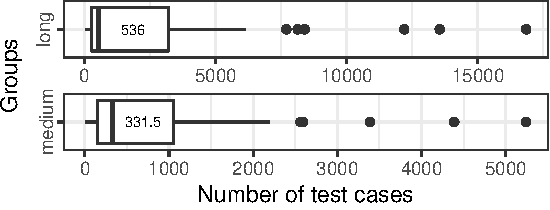
\includegraphics[width=.85\textwidth]{plots/boxplots-testcases.pdf}
    \caption{\label{fig:size-testsuites}Size of test suites.}
  \end{subfigure}
  ~
  \begin{subfigure}{0.3\textwidth}
    \centering
    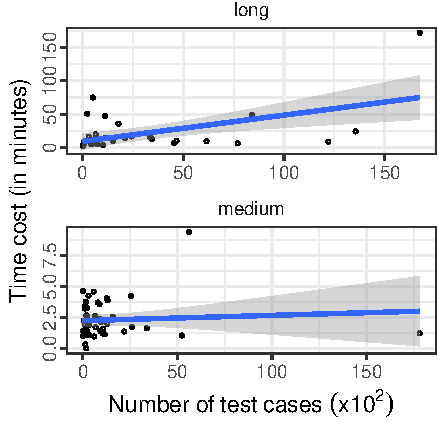
\includegraphics[width=.95\textwidth]{plots/scatter-testcost.pdf}
    \caption{\label{fig:scattercost}Size versus running time of
      test suites.}
  \end{subfigure}
  \caption{\label{fig:time-versus-size}Relating size and time.}%
\end{figure}

%\Mar{$\leftarrow$ show stats to indicate discrimination of
%  two distributions}

Figure~\ref{fig:time-distributions} showed that the average median
times were similar for \medg{} and \longg{}-running test suites.
Results indicate that the difference in overall running times of
projects in those groups was mainly justified by the number of test
cases as opposed to the individual costs of test cases.
Figure~\ref{fig:size-testsuites} shows the difference in the
distribution of test suite sizes across groups.  This figure indicates
that long projects, albeit having a wider inter-quartile range (middle
50\% projects in this group are less predictable), have a higher
median and much higher average number of test cases.  Furthermore, we
noted a strong positive correlation between running time and number of
test on projects in the \longg{} group.  Considering the \medg{}
group, the correlation between these two variables was weak.
Figure~\ref{fig:scattercost} illustrates this correlation.

%% however, weak in
%% the suggesting that saving time in this group with test suite
%% parallelization may be more challenging as relatively fewer tests
%% dominate overall execution time.  Figure~\ref{fig:scattercost} shows
%% these results.

%% This 
%% indication that it is more beneficial to parallelize long projects as
%% cost is spread across many

\vspace{1ex}
\begin{center}
\fbox{
\begin{minipage}{8cm}
    \textit{Answering \numRQFeasibilityTwo{}:}~\emph{Overall, results indicate that
    projects with a very small number of tests monopolizing end-to-end
    execution time were rare.}
\end{minipage}
}
\end{center}
\vspace{1ex}

%% We are interested to know whether
%% most of the execution cost of a subject is dominated by a small subset
%% of test cases or if the cost is nearly equally distributed. 

%% We also evaluated the dispersion of time distributions (one
%% distribution per project) to answer research question \numRQFeasibilityTwo{}.  To
%% measure dispersion \emph{across} projects we used Relative Standard
%% Deviation (RSD)~\cite{everitt-book-stats-2010}.  Note that, if we were
%% to analyze each project in isolation, the standard deviation of a
%% distribution ($\sigma$) would suffice to quantify how dispersed the
%% (time) distribution is.  However, in our case, we would like to be
%% able to compare and summarize dispersion across projects.  The RSD,
%% which is obtained dividing the standard deviation by the mean ($\mu$)
%% of a distribution, provides such normalization effect.  This metric
%% provides a lower bound (zero) but not an upper bound (somewhere close
%% to 1).  The smaller (larger) the value of RSD the more (less) uniform
%% the distribution is.  Consequently, the lower the value of RSD the
%% more parallelizable a test suite should be.

%% \begin{figure}[h!]
%%   \centering
%%   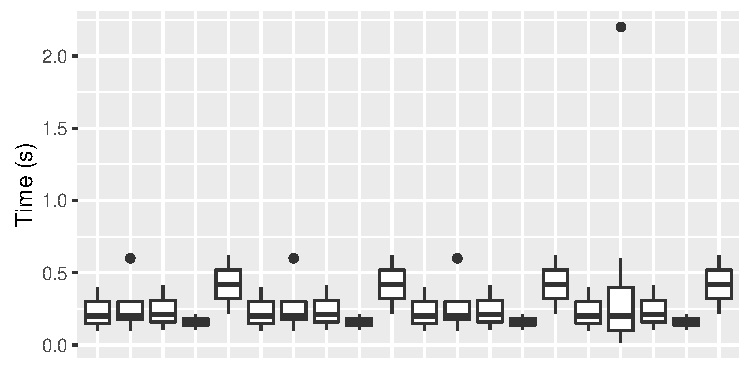
\includegraphics[width=0.5\textwidth]{R/testcost.pdf}  
%%   \caption{\label{fig:relativesd}Distribution of RSD ($\sigma/\mu$)
%%     across projects.}
%% \end{figure}

%% Figure~\ref{fig:relativesd} shows the distribution of RSD across
%% medium and long-running projects.  Results show that the distribution
%% is skewed to the right indicating that test costs are relatively well
%% distributed in most costly projects we analyzed \Fix{$\leftarrow$
%%   confirm}.

%% analyzed the execution time
%% for the \numMedLong{} projects from the \longg{} and \medg{} groups
%% (see Section~\ref{sec:rqA}).
%% For each subject we calculated the
%% relative standard deviation of the test cases: we collected the
%% elapsed time of each individual test, calculated the standard
%% deviation, and divided by the mean. \Jbc{I need to clarify the
%%   relationship "well/bad-balanced" regression test and relative
%%   standard deviation}

%% Results indicated that \Fix{...elaborate...}. \Jbc{We may identify
%% different groups of subjects}\Fix{TODO: collect data + compute the
%% statistic, create a scatter plot to identify groups of subjects}

%% Regression tests that are well distributed may benefit from
%% parallelism since more tests executes at the same time while the
%% opposite scenario may require a different approach. In the later
%% scenario, executing tests in parallel may have insignificant impact
%% since a small subset of test cases dominates the execution.}


\subsection{Adoption}
\label{sec:rqC}
\label{sec:rqE}

The dimension adoption focuses on the usage of parallelism in
open-source projects.  It evaluates (\numRQAdoptionOne) how often open-source
projects use parallelization schemes and (\numRQAdoptionTwo) how developers
involved in costly projects, not using parallelization, perceive this
technology.

\begin{itemize}
    \item \numRQAdoptionOne. \textbf{\RQAdoptionOne{}}
\end{itemize}

To answer \numRQAdoptionOne{}, we selected all projects from the \medg{} and
\longg{} groups, \ie, projects that ran in at least one minute.  This
set includes \numMedLong{} projects (see Section~\ref{sec:rqA}).  We
looked for dynamic and static manifestations of parallelism.

%% The
%% following section report results for each of these cases.

\vspace{1ex}
\subsubsection{Dynamic checking}
\label{sec:rqC-1}

To find dynamic evidence of parallelism, we ran the test suites from
our set of \numMedLong{} projects to output all key-value pairs of
Maven parameters.  To that end, we used the option~\CodeIn{-X} to
produce debug output and the option~\CodeIn{-DskipTests} to skip
execution of tests.  We skipped execution of tests as we observed from
sampling that only bootstrapping the Maven process suffices to infer
which parallel configuration modes it will use to actually run the
tests.  It is also important to point that we used the default
configurations specified in the project.  We inferred parallel
configurations by searching for certain configuration parameters in
log files. According to Maven's
documentation~\cite{maven-surefire-plugin}, a parallel configuration
depends either on (1) the parameter \CodeIn{parallel} to define the
parallelism mode within a JVM followed by the parameter
\CodeIn{threadCount} or (2) the parameter
\CodeIn{forkCount}\footnote{This parameter is named \CodeIn{forkMode}
  in old versions of Maven Surefire} to define the number of forked
JVMs.  As such, we captured, for each project, all related key-value
pairs of Maven parameters and mapped those pairs to one of the
possible parallelization modes.  For instance, if a given project
contains a module with the parameter
\CodeIn{<forkCount>1C</forkCount>}, the possible classifications are
\ForkSeq{} or \ForkParMeth{}, depending on the presence and the value
of the parameter \CodeIn{parallel}.  If the parameter
\CodeIn{parallel} is set to \CodeIn{methods} the detected mode will be
\ForkParMeth{}.  Large projects may contain several test suites
distributed on different Maven modules potentially using different
configurations.  For those cases, we collected the Maven output from
each module discarding duplicates as to avoid inflating counts for
configuration modes that appear in several modules of the same
project. For instance, if a project contains two modules using the
same configuration, we counted only one occurrence.


\begin{wrapfigure}{r}[0pt]{0pt}%0.525\linewidth
  \footnotesize
  %  \small
  \centering
  \setlength{\tabcolsep}{2.5pt}
%    \resizebox{.48\textwidth}{!}{%
    \begin{tabular}{lrr}
        \toprule
        \emph{Subject} & \emph{\# of modules} & \emph{Mode}\\%
        \midrule%
        \Comment{BounceStorage }Chaos\Comment{ HTTP Proxy} & 1/1 &  \ParClassSeqMeth{}\\%
        \Comment{Apache }Flink & 74/74 & \ForkSeq{} \\%        
        \Comment{JenkinsCI }Gerrit\Comment{ Trigger Plugin} & 1/1 & \ForkSeq{}\\%
        \Comment{Spotify }Helios & 8/8 & \ForkSeq{}\\%
        Javaslang & 3/3 & \ParClassParMeth{}\\%
        Jcabi\Comment{ Github} & 1/1 & \ParClassParMeth{}\\%        
        \Comment{Hazelcast }Jet & 7/14 & \ForkSeq{}\\%
        \Comment{Apache Logging }Log4J2 & 25/31 & \ForkSeq{}\\%
        \Comment{Jankotek }MapDB & 1/2 & \ParClassParMeth{}\\%        
        \bottomrule%
    \end{tabular}
    \caption{Subjects with parallel test execution enabled by
    default.}
    \label{tab:freqmodes-dynamic}
\end{wrapfigure}
Figure~\ref{tab:freqmodes-dynamic} shows the projects we idendified
where parallelism is enabled by default in Maven.  Column
``\emph{Subject}'' indicates the name of the project, column
``\emph{\# of modules}'' indicates the fraction of modules containing
tests that use the configuration of parallelism mentioned in column
``\emph{Mode}''.  We note that, considering these projects, the
modules that do not use the configuration cited use the sequential
configuration \Seq{}.  For example, six modules (=31-25) from Log4J2
use sequential configuration.

It came as a surprise the observation that
no project used distinct configurations in their modules. Considering
our set of \numMedLong{} projects, we found that only
\textbf{\numProjectsPar{}} of those projects had parallelism enabled
by default, with only configurations \ParClassSeqMeth{},
\ParClassParMeth{}, and \ForkSeq{} being used.  Configurations
\ParClassParMeth{} and \ForkSeq{} were the most popular among these
cases.  Note that these results under-approximate real usage of
parallelism as we used default parameters in our scripts to spawn the
Maven process.  That decision could prevent execution of particular
test modules.
%\begin{figure}[h!]
%    \centering
%    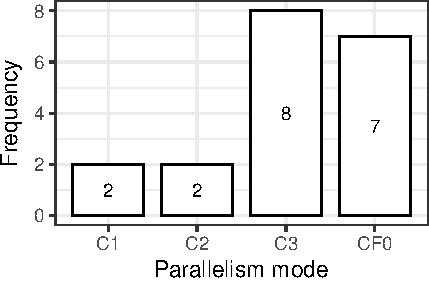
\includegraphics[width=0.32\textwidth]{plots/barplot-modes-dynamic.pdf}
%    \caption{\label{fig:freqmodes-dynamic}\Fix{fix
%    caption}Distribution of parallel modes identified dynamically in a
%    subset of \numProjectsPar{} projects.  A project may have support
%    to more than one parallel mode. Also, a project may run only a
%    subset tests in parallel by default.}
%\end{figure}

%% Recall that some projects can use parallel execution that is only
%% activated when developers pass certain parameters to the build
%% process. For instance, it is possible to create in Maven multiple
%% configurations in the same build file and select dynamically which one
%% should be used.  

\subsubsection{Static checking}
\label{sec:rqC-2}
Given the inherent limitation of dynamic monitoring to find evidence
of parallelism, we also looked for indication of parallelism in build
files\Comment{ in the same sample set of \numMedLong{} projects}.  We
parsed all \emph{pom.xml} files under the project's directory and used
the same approach as in our previous analysis to classify
configurations.  We noticed initially that our approach was unable to
infer the configuration mode for cases where the decision depends on
the input (\eg,
\CodeIn{<parallel>\$\{parallel.type\}</parallel>}). For these
projects, the tester needs to provide additional parameters in the
command line to enable parallelization (\eg, \CodeIn{mvn test
  -Dparallel.type=classesAndMethods}). To handle those case, we
considered all possible values for the parameter (in this case,
\CodeIn{\$\{parallel.type\}}).  It is also important to note that this
approach is not immune to false negatives, which can ocurr when
\emph{pom.xml} files are encapsulated in jar files or downloaded from
the network.  Consequently, this static checking is complementary to
the dynamic checking, previously presented.

Overall, we found, using this methodology, ten projects that use
parallelism.  Compared to the set of projects listed in
Figure~\ref{tab:speedup}, we found two new projects, namely:
\CodeIn{Google Cloud\Comment{ Platform} DataflowJavaSDK} (using
configuration C3) and \CodeIn{Mapstruct} (using configuration
\ForkSeq{}).  Curiously, we also found that project \CodeIn{Jcabi} was
not detected using this methodology.  That happened because this
project loads its \emph{pom.xml} file from a jar file that we did not
check.  Considering the static and dynamic methods together, we found
a total of 11 distinct projects using parallelism, corresponding to
the union of the two subject sets.

\vspace{1ex}
\begin{center}
\fbox{
  \begin{minipage}{8cm}
      \textit{Answering \numRQAdoptionOne{}:}~\emph{Results indicate that test
        suite parallelization is underused.  Overall, only
        \percentParallel{} of costly projects (11 out of \numMedLong)
        use parallelism.}
  \end{minipage}
}
\end{center}
\vspace{1ex}

%False positive can happen because of comments, for instance.  
%To eliminate the cases of false positives and also to categorize 
%true positive cases, we complemented the initial mining step with a 
%manual inspection of files.
%% settings); the second step (inspection) consists in a manual
%% inspection to confirm the presence of parallelism settings in the
%% build file and classify them according to the parallelism level.
%% Figure \Fix{removed} describes the discovery step: we list the paths
%% of all build files and filter only the files that contain any of the

%% Figure~\ref{tab:inspection-table} summarizes our results.
%% \Fix{The first column indicates the group of projects according to
%% their time cost.  The second column indicates the number of build
%% files per group.  The last column indicates the ratio of projects with
%% parallelization settings.  From the \numMedLong{} subjects, we found
%% \pomMedLong{} \pomf{} files.  The \numPomMatched{} configurations are
%% distributed across \numProjectsPar{} projects from our sample.}

%% % \emph{From these results we found that $\sim$51\% of medium and
%% % long-running projects do not use parallel features to run test
%% % suites.}\Mar{please make it consistent with research
%% % question}\Mar{explain this is over(under)-estimated...}
%% \begin{figure}[ht!]
%%     \centering
%%     \resizebox{.48\textwidth}{!}{%
%%     \begin{tabular}{llcl}
%%         \toprule
%%         Group & Subject & \# of modules & Mode\\%
%%         \midrule%
%%         Long   &JenkinsCI Gerrit Trigger Plugin& 1 & \ForkSeq\\%
%%         Medium &Bouncestorage Chaos Http Proxy & 1 & C2\\%
%%         Medium &Javaslang & 1 & C3\\%
%%         Medium &Apache Flink & 1 &\ForkSeq\\%
%%         Medium &Apache Logging Log4J2 & 3 & \ForkSeq{}\\%
%%         Medium &Google Cloud Platform DataflowJavaSDK & 1 & C3\\%
%%         Medium &Hazelcast Jet & 1 & \ForkSeq\\%
%%         Medium &Jankotek MapDB & 1 & C3\\%
%%         Medium &Mapstruct & 1 & \ForkSeq\\%
%%         Medium &Spotify Helios & 3 & \ForkSeq\\%
%%         \bottomrule%
%%     \end{tabular}}
%%     \caption{Subjects with parallelization configurations in build files.}
%%     \label{tab:inspection-table}
%% \end{figure}

%% \begin{figure}[ht!]
%%     \centering
%%     \begin{tabular*}{0.48\textwidth}{@{\extracolsep{\fill}}ccc}
%%         \toprule
%%         \multirow{2}{*}{Group} %1st row, 1st cell
%%             & \multirow{2}{*}{\# \pomf{}}
%% 	    & \# \pomf{} matched\\
%%         % 2nd row - empty cell
%%             & % empty cell
%%             & / total\\%
%%         \midrule%
%% 	Long   & \numPomLong{} & 4 / \numLong{}\\%
%% 	Medium & \numPomMed{} & 6 / \numMed{}\\%
%%         \midrule%
%%         Total % last row, first cell
%%             & \pomMedLong{}
%%             & \numProjectsPar{} / \numMedLong{}\\%
%%         \bottomrule%
%%     \end{tabular*}
%%     \caption{Presence of parallelization settings in build files: the
%%     first column indicates the group of projects according to their
%%     time cost; the second column is the subset of files with parallelization
%%     keywords; the last column indicates the ratio of projects with
%%     parallelism support.}
%%     \label{tab:inspection-table} 
%% \end{figure}
%% \Jbc{rework this... $\rightarrow$} From the \numProjectsPar{} projects
%% identified above, we investigated further the \numPomMatched{}
%% build files with parallel settings.  We analyzed the support and
%% distribution of parallel modes from this subset of projects. To
%% calculate the distribution of parallel modes, we considered only the
%% presence of the mode in at least one of the project settings.  Recall
%% that a build file may contain more than one parallel setting and a
%% project may contain several sub-modules with build files.  In case the
%% value of a parallel option is resolved dynamically (\eg, via
%% command-line argument or system variable) we compute all modes related
%% to the option. For instance, depending on the value, the
%% \CodeIn{parallel} option can be \Seq{} (\CodeIn{none}),
%% \ParClassSeqMeth{} (\CodeIn{classes}), \SeqClassParMeth{},
%% (\CodeIn{methods}), and \ParClassParMeth{} (\CodeIn{all}).
%% Figure~\Fix{fig:freqmodes-static} summarizes our findings.
%% \Fix{Missing conclusion: Fork the most used configuration}
%% \begin{figure}[h!]
%%     \centering
%%     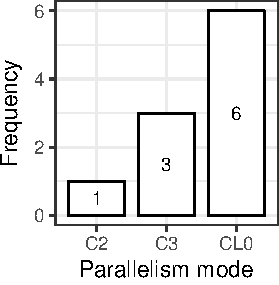
\includegraphics[width=0.32\textwidth]{plots/barplot-modes-static.pdf}
%% 	\caption{\label{fig:freqmodes-static}\Luis{This is wrong, it
%% 	should be \textbf{CF0} instead of \textbf{CL0}}Distribution of parallel modes
%%     identified statically in a subset of \numProjectsPar{} projects.
%%     A project may have support to more than one parallel mode.}
%% \end{figure}


\begin{itemize}
	\item \numRQAdoptionTwo{}. \textbf{\RQAdoptionTwo{}}
\end{itemize}

To answer this research question we surveyed developers involved in a
selection of projects from our benchmark with time-consuming test
suites.  The goal of the survey is to better comprehend developer's
attitude towards the use of parallelism as a mechanism to speedup
regression testing.  We surveyed developers from a total of
\emailsProjects{} projects.  From the initial list of \numMedLong{}
project, we discarded 11 projects that we knew a priori used
parallelization, and \discartedProjects{} projects that we could not find
developer's emails from commit logs.  From this list of projects, we
mined potential participants for our study.  More precisely, we
searched for developer's name and email from the last 20 commits to
the corresponding project repository.  Using this approach, we
identified a total of \emailsSent{} eligible participants.  Finally,
we sent plain-text e-mails, containing the survey, to those developers.  In
total, \emailsAnswered{} developers replied but we discarded
\emailsFalseAnswers{} replies with subjective answers.  Considering
projects covered by the answers, a total of \emailsProjectsAnswered{}
projects (\percEmailsProjectsAnswered{} of the total) were represented
in those replies.  Note that multiple developers on each project
received emails.  We sent the following set of questions to
developers:

\begin{enumerate}
\item How long does it take for tests to run in your environment? Can
  you briefly define your setup?
\item Do you confirm that your regression test suite does *not* run in parallel?
\item\label{questionThree} Select a reason for not using parallelization:
  \begin{enumerate}[label=\alph*)]
  \item I did not know it was possible
  \item I was concerned with concurrency issues
  \item I use a continuous integration server
  \item Some other reason. Please elaborate.
  \end{enumerate}
\end{enumerate}

%% \begin{enumerate}
%% 	\item How long does it take for test to run in your
%%		environment?
%%	\item Can you briefly define your setup?
%%	\item Do you confirm that your project does not run in
%%		parallel?
%%	\item Select a reason for not using paralellization:
%%		\begin{enumarate}
%%			\item I did not know it was possible;
%%			\item I was concerned with concurrency issues;
%%			\item I use a continuous integration server;
%%			\item Some other reason.
%%		\end{enumerate}
%% \end{enumerate}
%% One of the goals of the first questions is to identify potential
%% discrepancies between our experimental environment and the environment
%% of developers.  Overall, we found that \Fix{...}

Considering question 1, we confirmed that execution time was
compatible with the results we reported in Section~\ref{sec:rqA}.
Furthermore, \emailsCI{} of the participants indicated the use of
Continuous Integration (CI) to run tests, with \emailsDistributed{} of
these participants reporting that test suites are modularized and
those modules are tested independetly in CI servers through different
parameters.  Those participants argumented that such practice helps to
reduce time to observe test failures, which is the goal of speeding up
regression testing.  A total of \emailsLocal{} participants answered
that they do run tests in their local machines.  Note, however, that
CI does not preclude low-level parallelization.  For example,
installations of open-source CI tools (\eg{}, Jenkins~\cite{jenkins})
in dedicated servers would benefit from running tests faster through
low-level test suite parallelization.

% \emailsNotDescribed{} developers did not described their environment.

Considering question 2, the answers we collected indicated, to our
surprise, that six of the \emailsProjectsAnswered{} projects execute
tests in parallel.  This mismatch is justified by cases where neither
of our checks (static or dynamic) could detect presence of
parallelism.  A closer look at these projects revealed that one of
them contained a \emph{pom.xml} file encapsulated in a jar file
(similar case as reported in Section~\ref{sec:rqC-2}), in one of the
projects the particpant considered that distributed CI was a form of
parallelism, and in four projects the team preferred to implement
parallelization instead of using existing features from the testing
framework and the build system~---~in two projects the team
implemented concurrency control with custom JUnit test runners and in
two other projects the team implemented concurrency within test
methods.  Note that, considering these four extra cases (ignored two
distributed CI cases), the usage of parallelization increases from
\percentParallel{} to \percentParallelUpdated{}.  We do not consider
this change significant enough to modify our conclusion about
practical adoption of parallelization (\numRQAdoptionOne{}).

%% , one runs a manually created Thread to run some
%% tests, and the other runs in parallel by using Java 8 collection
%% streams, that allows the developers to iterate over a list in
%% parallel.

%% did not confirmed, however,
%% the developers confirmed the need of an extra parameter at the command
%% line to execute in parallel.

Considering question 3, the distribution of answers was as follows.  A
total of \emailsA{} of the \emailsProjectsAnswered{} developers who
answered the survey did not know that parallelism was available in
Maven (option ``a''), \emailsB{} of developers mentioned that they did
not use parallelism concerned with possible concurrency issues (option
``b''), \emailsD{} of developers mentioned that continuous integration
services sufficed to provide timely feedback while running only smoke
\begin{wrapfigure}{r}[0pt]{0pt}%0.525\linewidth
    \centering
    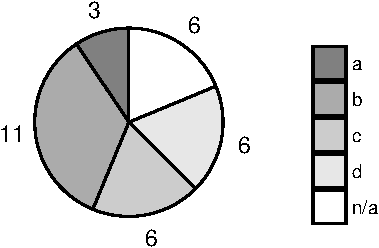
\includegraphics[width=.18\textwidth]{plots/survey.pdf}
    \caption{\label{fig:rq5-answers}Summary of developer's answers to
      survey question~\ref{questionThree}.}
\end{wrapfigure}
tests (\ie{}, short-running tests) locally (option ``c'')\Comment{here
  I want to say that they use it for something like "non-blocking
  testing" while developing in a local machine}, and \emailsD{} of
developers who provided an alternative answer (option ``d'') mentioned
that using parallelism was not worth the effort of preparing the test
suites to take advantage of available processing power.  A total of
\emailsNA{} of participants did not answer the last question of the
survey.  The pie chart in Figure~\ref{fig:rq5-answers} 
summarizes the distribution of answers.

\begin{center}
\fbox{
	\begin{minipage}{8cm}
	  \textit{Answering \numRQAdoptionTwo{}:}~\emph{Results suggest that dealing
       with concurrency issues (\ie{}, the extra work to organize test
       suite to safely explore concurrency) was the principal reason
       for developers not investing in parallelism.  Other reasons
       included availability of continuous integration services and
       unfamiliarity with the technology.}
	\end{minipage}
}
\end{center}

\subsection{Speedups}
\label{sec:rqD}

\begin{itemize}
    \item \numRQSpeedupOne{}. \textbf{\RQSpeedupOne}
\end{itemize}

To answer \numRQSpeedupOne{}, we considered the \numProjectsPar{}
subjects from our benchmark that use parallelization \emph{by default}
(see Figure~\ref{tab:freqmodes-dynamic}).  We compared running times
with parallelization~---~configured by project owners~---~and without
parallelization.

%% In those projects, parallelization is active without
%% passing any extra parameters.  Section~\ref{sec:rqC-1} describes in
%% detail the methodology we used to find these subjects.
%and
%Section~\ref{seq:rq6-tradeoffs}, we verified that both
%% executions produce the same outcome to eliminate noise from failing
%% tests.  To compute the speedup, we divide the time obtained in the
%% sequential execution by the time obtained from the default execution.
%% For instance, if a project runs the tests sequentially in $10m$ and
%% the same execution runs in $5m$ with parallelization enabled (default
%% execution), the speedup is two.

Figure~\ref{tab:speedup} summarizes results.  Lines are sorted by
project names.  Columns ``\emph{Group}'' and
``\emph{Name}'' indicate, respectively, the group and the name of the
subject.  Column ``$T_s$'' shows sequential execution time and column
``$T_p$'' shows parallel execution time. Column ``$T_s/T_p$'' shows
speedup or slowdown.  As usual, a ratio above 1x denotes speedup
and a ratio below 1x denotes slowdown.

\begin{figure}[h!]
\centering
\resizebox{.41\textwidth}{!}{%
  \scriptsize
\begin{tabular}{llrrr}
\toprule
\emph{Group} & \emph{Subject} & \multicolumn{1}{c}{$T_s$} & \multicolumn{1}{c}{$T_p$} & $T_s/T_p$ \\%
\midrule%
Medium & \Comment{BounceStorage }Chaos\Comment{ HTTP Proxy} & 1.51m & 1.47m & 
    \cellcolor{lightgray}1.01x\\%
Medium &\Comment{ Apache }Flink& 11.79m & 2.57m & 4.59x\\%
Long &\Comment{ Jenkins CI }Gerrit\Comment{ Plugin} & 51.19m & 40.31m &  1.26x\\%
Medium &\Comment{ Spotify }Helios& 4.46m & 1.63m & 2.73x\\%  
Medium &Javaslang& 2.18m & 1.82m & 1.19x\\%
Medium &Jcabi\Comment{ GitHub} & 2.76m & 0.30m &
    \cellcolor{lightgray}9.2x\\%
Medium &\Comment{ Hazelcast }Jet& 8.26m & 3.67m & 2.25x\\%
Long &\Comment{ Apache }Log4J2& 8.24m & 8.21m & \cellcolor{lightgray}1.00x\\%
Long &\Comment{ Jankotek }MapDB& 10.06m & 8.58m & 1.17x\\%
\midrule
\textbf{average} &  &  &  & \avgSpeedup{}x\\
\bottomrule%
\end{tabular}}
\caption{\label{tab:speedup}Speedup (or slowdown) of parallel
  execution ($T_p$) over sequential execution ($T_s$).  Default
  parallel configuration of Maven is used.  Highest slowdown/speedup
  appears in gray color.}
\end{figure}

Results indicate that, on average, parallel execution was
\avgSpeedup{} times faster compared to sequential execution.  Three
cases worth special attention: \CodeIn{Chaos}, \CodeIn{Jcabi} and
\CodeIn{Log4J2}.  No significant speedup was observed in
\CodeIn{Chaos}, a project with only three test classes, of which one
monopolizes the bulk of test execution time.  This project uses
configuration \ParClassSeqMeth{}, which runs test classes in parallel
and test methods, declared in each class, sequentially.  Consequently,
speedup cannot be obtained as the cost of the single expensive test
class cannot be broken down with the selected configuration.  Although
project \CodeIn{Jcabi} also uses configuration \ParClassSeqMeth{},
results obtained are very different compared to \CodeIn{Chaos}.  The
speedup observed in \CodeIn{Jcabi} was the highest amongst all
projects.  This project contains test classes with a small number of
test methods and several methods in those classes are time-consuming.
As result, the CPUs available for testing are kept occupied for the
most part during test execution.  Finally, we note that parallel
execution in \CodeIn{Log4J2} was innefective.  We found that Maven
invokes several test modules in this project but the test modules that
dominate execution time run sequentially by default.

%% The third, runs parallel configuration in
%% \Fix{80\%} of the project modules, however, the test time is dominated
%% by one of the sequentially running modules.  \Luis{$\leftarrow$ rework
%%   this} \Fix{falar sobre o resultado geral dos speedups - elaborar
%%   menor e maior speedup... acho que so vale a pena discutir quando
%%   tiver conviccao dos 2 casos}

\begin{center}
\fbox{
  \begin{minipage}{8cm}
    \textit{Answering \numRQSpeedupOne{}:}~\emph{Considering the
      machine setup we used, the average speedup observed with default
      configurations of parallelization was \avgSpeedup{}x.}
  \end{minipage}
}
\end{center}

\begin{itemize}
    \item \numRQSpeedupTwo{}. \textbf{\RQSpeedupTwo}
\end{itemize}

\newcommand{\subjectScalability}{MapDB}

This experiment evaluates the impact of making available to the build
system a growing number of CPUs for testing.  For that reason, we used
a machine with more cores compared to the one described in
Section~\ref{sec:setup}.  We used a Xeon E5-2660v2 (2.20GHz) Intel
processor machine with 80 virtual CPUs (40 cores with two native
threads each) and 256GB of memory, running Ubuntu 14.04 LTS Trusty
Tarr (64-bit version). This experiment uses configuration \ForkSeq{}
\begin{wrapfigure}{r}[0pt]{0pt}%0.525\linewidth
    \centering
    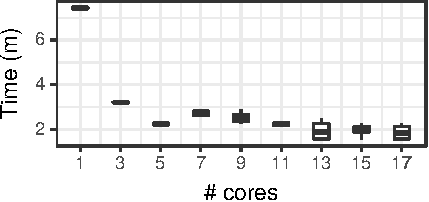
\includegraphics[width=.2\textwidth]{R/scalability/scalability.pdf}
    \caption{\label{fig:scalability}Scalability.}
\end{wrapfigure}
as the goal is to evaluate the impact on runtime of spawning a growing number of
JVMs in different CPUs.  Furthremore, we selected subject
\subjectScalability{} as it represents the case of a long-running test
suite (see Figure~\ref{tab:speedup}) with test cases distributed
across many test classes (194 test classes for \subjectScalability{}).
Note that a test class is the smallest unit that can be used to spawn
a test job on a JVM and that we have no control over which test
classes will be assigned to which JVM that the build system forks.

Figure~\ref{fig:scalability} shows the reduction of running times as
more CPUs contribute to the execution.  \Fix{elaborate...}

\begin{center}
\fbox{
  \begin{minipage}{8cm}
    \textit{Answering \numRQSpeedupTwo{}:}~\emph{...}
  \end{minipage}
}
\end{center}

\subsection{Issues}
\label{sec:rq6-tradeoffs}

This dimension assesses the impact of using distinct parallel
configurations on test flakiness (negative impact) and speedup
(positive impact).  Furthermore, note that Section~\ref{sec:rqD}
evaluated speedup in isolation, focused on projects configured to use
parallelism by default.

\begin{itemize}
    \item \numRQIssuesOne{}. \textbf{\RQIssuesOne{}}
\end{itemize}


%% The intuition is that efficiency and flakiness are inversely
%% proportional in some cases: if too many tests depends on the state of
%% a single external resource, several tests are likely to fail as the
%% degree of concurrency increases by exploiting maximum CPU usage.

%% Table header macros
% $\Uparrow_\text{speed}$
\newcommand{\subcolA}{$\text{speedup}$}
\newcommand{\subcolB}{$\%_\text{fail}$}
\newcommand{\colheader}[1]{\multicolumn{2}{c}{\emph{#1}}}
\newcommand{\blankentry}{\entry{-}{-}}
\newcommand{\subcol}{\subcolA{} & \subcolB{}}
\newcommand{\entry}[2]{#1 & #2}

\begin{figure*}[t]  
\centering
\small
\setlength{\tabcolsep}{3pt}
\begin{tabular}{l|rr|rr|rr|rr|rr|rr}
\toprule
\multirow{2}{*}{\emph{Subject (module)}} & \multicolumn{2}{c|}{\emph{\Seq}} &
    \colheader{\SeqClassParMeth} & \colheader{\ParClassSeqMeth} &
    \colheader{\ParClassParMeth} & \colheader{\ForkSeq} &
    \colheader{\ForkParMeth} \\ %\cline{2-12}
    & $T$ & $\mathit{N}$ & \subcol{} & \subcol{} & \subcol{} & \subcol{}
    & \subcol{}\\%
\midrule%
AWS SDK Java (\CodeIn{core})  & \entry{3.7m}{847}  & \entry{1.95x}{2.24\%} & \entry{2.47x}{2.77\%} & \entry{3.70x}{4.01\%} & \entry{}{} & \entry{}{}\\%

Facebook Linkbench    & \entry{4.3m}{98}  & \entry{1.00x}{0\%} & \entry{1.65x}{1.02\%} & \entry{1.59x}{1.02\%} & \entry{}{} & \entry{}{}\\%

GoogleCloud Dataflow Java (\CodeIn{sdk}) & \entry{1.6m}{3,345}  & \entry{1.23x}{1.67\%} & \entry{2.67x}{1.05\%} & \entry{0.80x}{5.35\%} & \entry{}{} & \entry{}{}\\%

Javaslang (\CodeIn{core})     & \entry{1.1m}{17,513}  & \entry{1.38x}{0\%} & \entry{1.83x}{0\%} & \entry{1.38x}{0\%} & \entry{}{} & \entry{}{}\\ 
JCabi Github                  & \entry{2.6m}{634} & \entry{2.10x}{0\%} & \entry{17.70x}{0\%} & \entry{28.80x}{0\%} & \entry{}{} & \entry{}{} \\
JCTools (\CodeIn{core})       & \entry{3.6m}{690}  & \entry{4.50x}{0\%} & \entry{3.60x}{0\%} & \entry{18.00x}{0\%} & \entry{}{} & \entry{}{}\\%
MapDB  & \entry{8.2m}{5,324}  & \entry{1.52x}{0\%} & \entry{2.73x}{0\%} & \entry{4.82x}{0.05\%}   & \entry{}{} & \entry{}{}\\%
Moquette                      & \entry{3.7m}{169} & \entry{4.62x}{65.64\%} & \entry{3.36x}{32.92\%} & \entry{12.33x}{77.78\%} & \entry{}{} & \entry{}{} \\
RipMe                         & \entry{1.1m}{54}  & \entry{0.94x}{0\%} & \entry{1.63x}{0\%} & \entry{1.63x}{0\%} & \entry{1.37x}{0\%} & \entry{1.42x}{0\%}\\
Stripe Java     & \entry{4.3m}{302}  & \entry{4.78x}{6.31\%} & \entry{3.31x}{7.31\%} & \entry{21.50x}{14.95\%} & \entry{}{} & \entry{}{}\\%





\midrule

\textbf{Average}   & \entry{-}{-} & \entry{-}{-} & \entry{-}{-} & \entry{-}{-}
& \entry{-}{-} & \entry{-}{-} \\%


%%  & \entry{x.xm}{0}  & \entry{}{\%} & \entry{}{\%} & \entry{}{\%} & \entry{}{} & \entry{}{}\\%
%%OpenMRS Core (\CodeIn{api})  & \entry{15.4m}{3436} & \blankentry{}        & \blankentry{}        & \blankentry{} & \entry{1.5x}{0\%} & \entry{1.7x}{0}\\%
%%Apache Flume (\CodeIn{core}) &  \entry{7.7m}{392}  & \blankentry{}        & \blankentry{}        & \blankentry{}       & \entry{0.9x}{0\%} & \blankentry{} \\%
%%Facebook Archive Linkbench   &  \entry{4.5m}{98}   & \entry{1.0x}{0.2\%}  & \entry{1.6x}{1.2\%}       & \entry{1.0x}{0\%}  & \entry{1.7x}{0.5\%}  & \entry{1.7x}{0.2\%}\\%
%%AWS SDK Java (\CodeIn{core}) &  \entry{3.8m}{847}  & \multicolumn{6}{c}{\Fix{requires investigation}} & \entry{2.2x}{0.1\%} & \entry{3.2x}{2.0\%}\\%

%% OpenMRS Core (\CodeIn{api})  & \entry{15.4m}{3436} & \blankentry{}        & \blankentry{}        & \blankentry{} & \entry{1.5x}{0\%} & \entry{1.7x}{0}\\%
%% Jankotek MapDB               &  \entry{9.9m}{5218} & \multicolumn{6}{c}{\cellcolor{lightgray}\emph{JVM Crash}} & \entry{1.5x}{0\%} & \entry{1.7x}{0\%}\\%
%% Apache Flume (\CodeIn{core}) &  \entry{7.7m}{392}  & \blankentry{}        & \blankentry{}        & \blankentry{}       & \entry{0.9x}{0\%} & \blankentry{} \\%
%% Apache Giraph (\CodeIn{core})&  \entry{7.2m}{236}  & \entry{2.1x}{5.1\%}  & \colheader{\cellcolor{lightgray}timeout}   & \entry{1.0x}{0\%} & \entry{1.0x}{0}\% & \colheader{\cellcolor{lightgray}JVM Crash}\\%
%% Facebook Archive Linkbench   &  \entry{4.5m}{98}   & \entry{1.0x}{0.2\%}  & \entry{1.6x}{1.2\%}       & \entry{1.0x}{0\%}  & \entry{1.7x}{0.5\%}  & \entry{1.7x}{0.2\%}\\%
%% Stripe Java                  &  \entry{4.2m}{302}  & \entry{4.2x}{5.2\%}  & \entry{3.5x}{5.7\%}       & \entry{4.2x}{6.3\%} & \entry{1.0x}{0.3\%} & \entry{4.2x}{5.7\%}\\%
%% AWS SDK Java (\CodeIn{core}) &  \entry{3.8m}{847}  & \multicolumn{6}{c}{\Fix{requires investigation}} & \entry{2.2x}{0.1\%} & \entry{3.2x}{2.0\%}\\%

%% Jenkins CI Github            & \entry{Xm}{Z}       & \entry{x}{\%}          & \entry{x}{\%} & \entry{x}{\%} & \entry{x}{\%} & \entry{x}{\%}\\%
%% Jenkins CI Docker Workflow   & \entry{Xm}{Z}       & \entry{x}{\%}          & \entry{x}{\%} & \entry{x}{\%} & \entry{x}{\%} & \entry{x}{\%}\\%
%% Hazelcast                    & \entry{Xm}{Z}       & \entry{x}{\%}          & \entry{x}{\%} & \entry{x}{\%} & \entry{x}{\%} & \entry{x}{\%}\\%

\bottomrule%
\end{tabular}
\caption{Speedup versus Flakiness (\subcolB). Configuration
  \emph{\Seq{}} denotes the comparison baseline, which runs tests
  sequentially.  Columns $T$ and $N$ indicate time and number of
  tests, respectively.  Other columns show speedup and percentage of
  failing tests in different configurations, compared to
  \emph{\Seq{}}.\Mar{Can you please add name of module for all subjects?}}
\label{tab:rq6-table}
\end{figure*}

To answer this research question, we conducted an experiment involving
the six parallel configurations from Section~\ref{sec:modes}  and the
top 10 long-running test modules from our sample set. The rationale
for this selection criteria was to maximize the chances of observing
speedup and flakiness, assuming that long-running tests also have many
tests. Indeed, we confirmed that test suites in these projects contain
at least 236 tests ($1,662.7$ in average). Also, we preferred to compare the
effect of a configuration over a single test module for projects with
multiple test modules.  Recall that large projects may contain several
test modules, and these modules may contain distinct characteristics
that could favor one configuration and not others; therefore, it would
be necessary to check each module individually for a fair comparison.
We are interested in understanding how efficiency (\ie, testing cost)
and flakiness (\ie, failing tests) are affected when we run a test
suite with different parallel configurations.  Recall that increased
resource contention obtained with parallelism can lead to concurrency
issues such as data races.  Flakiness and speedup are contradictory
forces that drive configuration selection.  We used as a \emph{control
group} (\ie, baseline) the sequential execution of each subject's
tests. Notice that for measuring flakiness, we have to consider only
tests that failed due to the concurrency in the parallel execution.
For that reason, we re-executed the tests in sequence ten times and
carefully verified that there are only passing tests in our baseline.
We considered ten as the number of re-executions based on the approach
used by Google reported in a previous work on test
flakiness~\cite{luo-etal-fse2014}.  To obtain parallel configurations,
we implemented a script that takes a subject and a configuration (\eg,
\ForkSeq{}) as inputs, and the script outputs the modified version of
the subject with the desired configuration. The workflow consists in
copying the project directory to a new directory, finding all existing
build files (\ie, \pomf{} files), and modifying all existing Maven
Surefire configurations with new values for the parameters
\CodeIn{parallel}, \CodeIn{forkCount}, and \CodeIn{threadCount} using
an XPath~\cite{xpath} library to manipulate XML documents. For
configurations with forked JVMs enabled (\ie, \ForkSeq{} and
\ForkParMeth{}), we changed the \CodeIn{forkCount} with the value
\CodeIn{1C} (\ie, one JVM per core).  To adjust the pool of threads
for parallelism within a JVM, we changed the parameter
\CodeIn{threadCount} with \Jbc{should we consider 2 as it is the
number of native threads per core OR 6 as it represents 3 Cores * 2
native threads?}.  To run the subjects and their respective variations
(\ie, the modified versions according to the parallelism
configuration), we used a similar approach as described in


Figure~\ref{fig:mvn-execution} except that we added a timeout of one
hour to run the tests. We used the \CodeIn{timeout}
command~\cite{timeout-cmd} to monitor the execution, and we configured
the command to dispatch a \emph{kill} signal if the test execution
exceeds the time limit. We imposed this time constraint to avoid
hanging indefinitely the experiment execution due to some thread
contention that may occur (\eg, deadlock). Finally, we saved each
execution log and XML test reports generated by Maven to collect the
execution time, the number of failing tests, and for reference to
analyze and diagnose outliers in our results. For efficiency, we
reported the speedup (\ie, $\Uparrow_\text{speed} = T_{\text{s}} /
T_{\text{p}}$) in average, and for flakiness, we reported the rate of
failing tests (\ie, $\mathit{\%_\text{fail} = failures / tests}$) in
average.  Figure~\ref{tab:rq6-table} summarizes the obtained results
ordered by the time cost (\ie, $T_\text{cost}$). \Fix{Remember to
explain efficiency cutoff, JVM crashes and timeout}

\Jbc{Lembrar que investigar o slowdown de Dataflow... os logs indicam que varios
dos testes que quebraram tentavam fazer uma autenticacao em algum servico.
Possivelmente o slowdown se deve ao tempo de resposta do servico quando
a autentiticao falha}

%% \begin{figure}[h!]
%% \centering
%% \resizebox{.48\textwidth}{!}{%
%% \begin{tabular}{lcrrrrr}
%% \toprule
%% \emph{Subject} & \emph{\# of tests} & \emph{\SeqClassParMeth{}} & \emph{\ParClassSeqMeth{}} & \emph{\ParClassParMeth{}} & \emph{\ForkSeq{}} & \emph{\ForkParMeth{}}\\%
%% \midrule%
%% Linkedin Pinot & 356 & - & - & - & - & -\\%
%% %% Jenkins CI Github Plugin & - & - & - & - & 0\% & -\\%
%% %% Kite SDK & - & - & - & - & - & -\\%
%% %% \Fix{!?} Apache Giraph & 327 & - & - & - & - & -\\%
%% %% OpenMRS Core & - & - & - & - & - & -\\%
%% %% Jenkins CI Docker Workflow Plugin & - & - & - & - & 0\% & -\\%
%% %% \Fix{Flaky} Apache Eagle & - & - & - & - & - & -\\%
%% %%Geotools & 7701 & - & - & - & - & -\\%
%% %%Kuromoji & 672 & - & - & - & - & -\\%
%% %%Atomix & 99 & - & - & - & - & -\\%
%% %%\Fix{Snazy OHC} & - & - & - & - & - & -\\%
%% %%\Fix{RoaringBitmap} & - & - & - & - & - & -\\%
%% \bottomrule%
%% \end{tabular}}
%% \caption{\Fix{Tabela de flakiness}}
%% \label{tab:rq6-flaky}
%% \end{figure}

\Fix{Elaborate results from efficiency}

\Fix{Elaborate results from flakiness}

\Fix{highlight special cases}

\Fix{Draw conclusions}

\begin{center}
\fbox{
\begin{minipage}{8cm}
\textit{Answering \numRQIssuesOne{}:~\emph{\Jbc{summarize findings...}}}
\end{minipage}
}
\end{center}

%%  LocalWords:  RQ occurence parallelization Tradeoffs API readme th
%%  LocalWords:  mvn clearcut escapeinside xleftmargin untestable LTS
%%  LocalWords:  framexleftmargin CPUs Tahr sysstat gh Vagrantfile
%%  LocalWords:  javadoc isolcpus JUnit's JUnitCore Gligoric boxplots
%%  LocalWords:  outliers apache uber chaperone facebookarchive
%%  LocalWords:  linkbench priori


We ran the test suite for each subject three times, reporting averaged
execution times in three ranges: tests that run within a minute
(\shortg{} group), tests that run in one to five minutes (\medg{}
group), and tests that run in five or more minutes (\longg{}
group). We followed a similar methodology to group projects by time as
Gligoric~\etal{}~\cite{gligoric-etal-issta2015} in their work on
regression test selection.\Comment{ and added the \medg{} group due to
  the variability of the time cost from subjects out of the \shortg{}
  group} Figure~\ref{fig:rq1-barplot} shows the number of projects in
each group.  As expected, \longg{} and \medg{} projects do not occur
as frequently as \shortg{} projects.  However, they do occur in
relatively high numbers.

Figure~\ref{fig:rq1-boxplot} shows cost distribution of test suites in
each group as boxplots.  Note that the y-ranges are different.  The
distribution associated with the \shortg{} group is the most
unbalanced (right skewed)\Comment{ with outliers closed to the \medg{}
  group}.  The test suites in this group ran in 15 or less seconds for
over 75\% of the cases.  Such scenarios constitute the majority of the
cases we analyzed.  Considering the groups \medg{} and \longg{},
however, we found many costly executions.  Nearly 75\% of the projects
from the \medg{} group take over 3.5 minutes to run and nearly 75\% of
the projects from the \longg{} group take $\sim$20 minutes to run.  We
found cases in the \longg{} group were execution takes over 50 minutes
to complete, as can be observed from the outliers (dots) in the plot.

%% the median from the
%% \medg{} group is nearly two minutes and most of the subjects run in
%% less than four minutes; most of the \longg{} group runs in less than
%% 25 minutes but has outliers that require more than 50 minutes to
%% execute.



\begin{figure}[ht]
    \centering
    \begin{subfigure}{0.182\textwidth}
        \centering
        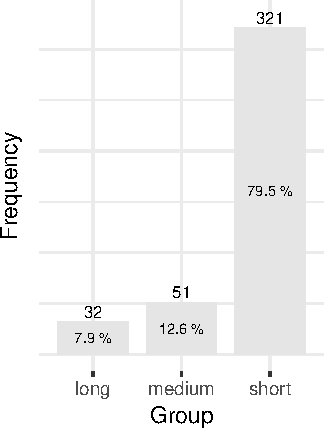
\includegraphics[width=\textwidth]{plots/barplot-timecost.pdf}
        \caption{\label{fig:rq1-barplot}}
    \end{subfigure}%
    ~
    \begin{subfigure}{0.25\textwidth}
        \centering
        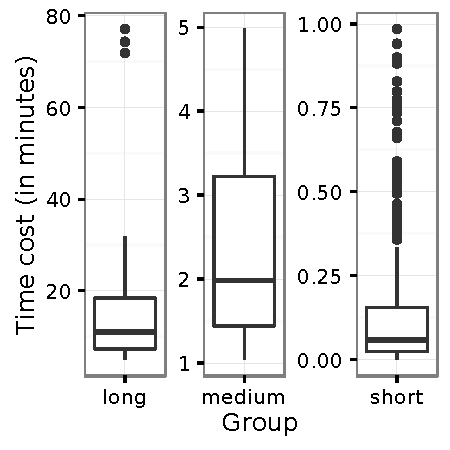
\includegraphics[width=\textwidth]{plots/boxplot-timecost.pdf}
        \caption{\label{fig:rq1-boxplot}}
    \end{subfigure}%
    \caption{(a) Subjects grouped by time cost ($t$): short run ($t <
    1m$), medium run ($1m \le t < 5m$), and long run ($5m \le t$); (b)
    Distribution of time cost by group.}
\end{figure}

%% Figure~\ref{fig:rq1-barplot} is a lower bound estimation of cost
%% because some tests may finish earlier than expected due to existing
%% test failures in the revision we downloaded.

It is important to note that we under-estimated cost in our
experiments for two main reasons.  First, some tests may finish
earlier than expected due to the observed test failures in some of the
revisions we downloaded.  From the \numSubjs{} testable projects,
\numSubjsPass{} successfully executed all tests and \numSubjsFail{}
reported some test failures.  Second, some projects may omit
long-running tests on their default execution. For instance, the
project \CodeIn{apache.maven-surefire} runs all unit tests in a few
seconds.  According to our criteria, this project is to be classified
as \shortg{} but a closer look reveals that only smoke tests are run
by default in this project.  Time-consuming integration and system
tests are only accessible via custom parameters, which we do not
handle in our experimental setup.  We enabled such parameters for this
specific project and observed that testing time goes to nearly 30
minutes.  For simplicity, we considered only the tests executed by
default.

\vspace{1ex}
\begin{center}
\fbox{
\begin{minipage}{8cm}
    \textit{Answering \numRQFeasibilityOne{}:}~\emph{We conclude that
      time-consuming test suites are relatively frequent in
      open-source projects.  We found that \percentMedLongRunning{} of
      the \numSubjs{} projects we analyzed (\ie{}, over 1 in every 5
      projects) take at least 3 minutes to run and
      \percentLongRunning{} take at least 5 minutes to run.\Comment{
        (\ie, \numMedLong{} projects from \medg{} and \longg{}).}}
\end{minipage}
}
\end{center}
\vspace{1ex}


\begin{itemize}
    \item \numRQFeasibilityTwo. \textbf{\RQFeasibilityTwo}
\end{itemize}

Section~\ref{sec:rqA} showed that medium and long-running projects are
not uncommon, accounting to nearly \percentMedLongRunning{} of the
\numSubjs{} projects we analyzed.  Research question \numRQFeasibilityTwo{}
measures the distribution of test costs in test suites as to estimate
(lack of) potential of obtaining speedups with parallelization.  In
the limit, if cost is dominated by a single test from a large test
suite, it is unlikely that parallelization will be beneficial as a
test method is the smallest working unit in test frameworks.

%% However, avoiding
%% frequent context switches is another factor to consider.  For example,
%% assuming there are at least two CPUs available for execution, cost can
%% be cut in half if two tests in a large test suite dominate execution
%% time and these tests are assigned to different CPUs.

%% It is therefore important to
%% speedup regressing testing in open-source projects.\Comment{not only
%%   to huge projects as those from Google~\cite{google-tap,google-ci}
%%   and Microsoft~\cite{prasad-shulte-ieee-microsoft-ci}.}



%% For the case
%% where cost is distributed more evenly across test cases, one expects
%% that speedups will be a function of the number of cores.
%% These contradictory forces, pushing number of tests and cost
%% of each test up and down, make prediction of effectiveness challenging.

\begin{figure}[h]
    \centering
    \begin{subfigure}{0.47\textwidth}
      \centering
      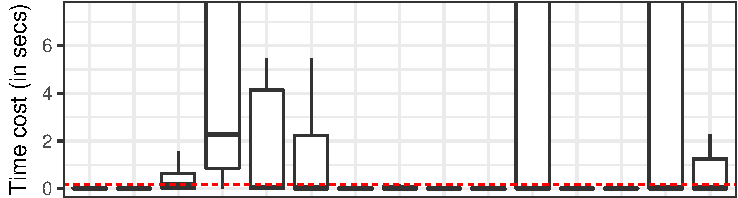
\includegraphics[width=\textwidth]{plots/testcost-long.pdf}
      \caption{\label{fig:longtcost}Long group.}
    \end{subfigure}\\
    \vspace{2ex}
    \begin{subfigure}{0.47\textwidth}
      \centering
      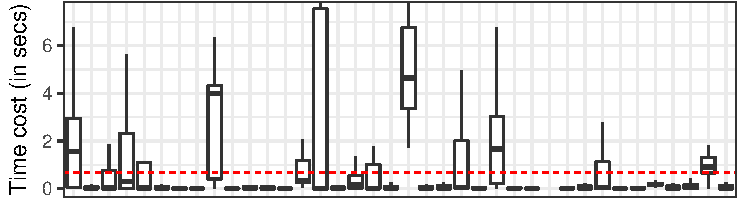
\includegraphics[width=\textwidth]{plots/testcost-medium.pdf}
      \caption{\label{fig:medtcost}Medium group.}
    \end{subfigure}
    %% \vspace{2ex}
    %% \begin{subfigure}{0.5\textwidth}
    %%   \centering
    %%   \begin{tabular}{rrrr}
    %%     \toprule
    %%     & $\sigma\leq1$ & $1<\sigma\leq5$ & $\sigma\ge5$ \\
    %%     \midrule    
    %%     Long   &  7 & 15 & 12 \\
    %%     Medium & 22 & 19 & 7 \\
    %%     \bottomrule
    %%   \end{tabular}
    %%   \caption{\label{fig:sd}Standard deviation ($\sigma$) of test case running times.}
    %% \end{subfigure}
    \caption{\label{fig:time-distributions}Time distributions.}%
\end{figure}

\sloppy Figures~\ref{fig:longtcost} and~\ref{fig:medtcost} show the
time distribution of individual test cases per project.  We observed
that the average median value of execution cost for a test was
relatively small (dashed horizontal red lines), namely 0.31s for
\medg{} projects and 0.23s for \longg{} projects.  The standard
deviations associated with each distribution were relatively
low.\Comment{ Figure~\ref{fig:sd} shows the number of projects within
  specific ranges of $\sigma$ values.}  We noted a small number of
cases of CPU monopolization.  For example, the highest value of
$\sigma$ occurred in \CodeIn{uber\_chaperone}, a project from the
medium group.  This project contains only 65 tests, 62 of which take
less than 0.5s to run, one of which takes nearly 3s to run, and two of
which take $\sim$40m to run.  For this project, 99.2\% of the
execution cost is dominated by only 3\% of the tests; without these
two costly tests this project would have been classified as
short-running.  A closer inspection in the data indicates that the
project \CodeIn{uber\_chaperone} was a corner case; we did not find
other projects with such extreme time monopolization profile.  Project
\CodeIn{facebookarchive\_linkbench} is also classified as long-running
and has the second highest value of $\sigma$.  For this project,
however, cost is distributed more smoothly across \Fix{529} tests, of
which \Fix{119 (23\%)} take more than \Fix{1s} to run with the rest of
the tests running faster.

\begin{figure}[t]
  \centering
  \begin{subfigure}{0.15\textwidth}
    \centering
    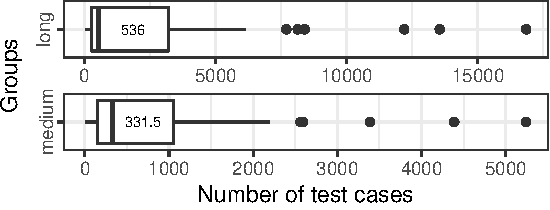
\includegraphics[width=.85\textwidth]{plots/boxplots-testcases.pdf}
    \caption{\label{fig:size-testsuites}Size of test suites.}
  \end{subfigure}
  ~
  \begin{subfigure}{0.3\textwidth}
    \centering
    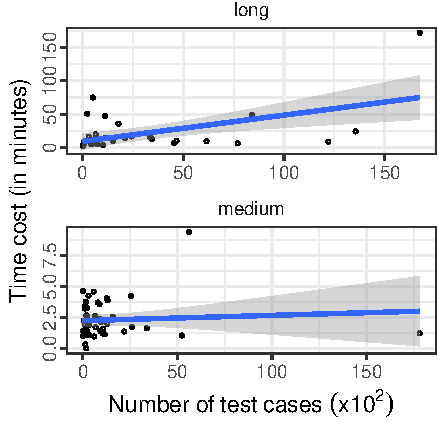
\includegraphics[width=.95\textwidth]{plots/scatter-testcost.pdf}
    \caption{\label{fig:scattercost}Size versus running time of
      test suites.}
  \end{subfigure}
  \caption{\label{fig:time-versus-size}Relating size and time.}%
\end{figure}

%\Mar{$\leftarrow$ show stats to indicate discrimination of
%  two distributions}

Figure~\ref{fig:time-distributions} showed that the average median
times were similar for \medg{} and \longg{}-running test suites.
Results indicate that the difference in overall running times of
projects in those groups was mainly justified by the number of test
cases as opposed to the individual costs of test cases.
Figure~\ref{fig:size-testsuites} shows the difference in the
distribution of test suite sizes across groups.  This figure indicates
that long projects, albeit having a wider inter-quartile range (middle
50\% projects in this group are less predictable), have a higher
median and much higher average number of test cases.  Furthermore, we
noted a strong positive correlation between running time and number of
test on projects in the \longg{} group.  Considering the \medg{}
group, the correlation between these two variables was weak.
Figure~\ref{fig:scattercost} illustrates this correlation.

%% however, weak in
%% the suggesting that saving time in this group with test suite
%% parallelization may be more challenging as relatively fewer tests
%% dominate overall execution time.  Figure~\ref{fig:scattercost} shows
%% these results.

%% This 
%% indication that it is more beneficial to parallelize long projects as
%% cost is spread across many

\vspace{1ex}
\begin{center}
\fbox{
\begin{minipage}{8cm}
    \textit{Answering \numRQFeasibilityTwo{}:}~\emph{Overall, results indicate that
    projects with a very small number of tests monopolizing end-to-end
    execution time were rare.}
\end{minipage}
}
\end{center}
\vspace{1ex}

%% We are interested to know whether
%% most of the execution cost of a subject is dominated by a small subset
%% of test cases or if the cost is nearly equally distributed. 

%% We also evaluated the dispersion of time distributions (one
%% distribution per project) to answer research question \numRQFeasibilityTwo{}.  To
%% measure dispersion \emph{across} projects we used Relative Standard
%% Deviation (RSD)~\cite{everitt-book-stats-2010}.  Note that, if we were
%% to analyze each project in isolation, the standard deviation of a
%% distribution ($\sigma$) would suffice to quantify how dispersed the
%% (time) distribution is.  However, in our case, we would like to be
%% able to compare and summarize dispersion across projects.  The RSD,
%% which is obtained dividing the standard deviation by the mean ($\mu$)
%% of a distribution, provides such normalization effect.  This metric
%% provides a lower bound (zero) but not an upper bound (somewhere close
%% to 1).  The smaller (larger) the value of RSD the more (less) uniform
%% the distribution is.  Consequently, the lower the value of RSD the
%% more parallelizable a test suite should be.

%% \begin{figure}[h!]
%%   \centering
%%   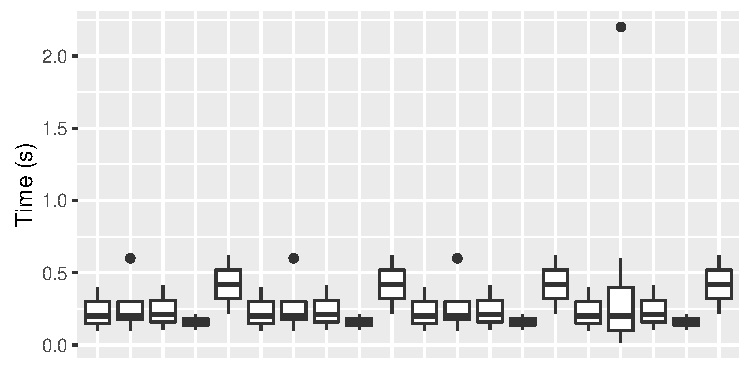
\includegraphics[width=0.5\textwidth]{R/testcost.pdf}  
%%   \caption{\label{fig:relativesd}Distribution of RSD ($\sigma/\mu$)
%%     across projects.}
%% \end{figure}

%% Figure~\ref{fig:relativesd} shows the distribution of RSD across
%% medium and long-running projects.  Results show that the distribution
%% is skewed to the right indicating that test costs are relatively well
%% distributed in most costly projects we analyzed \Fix{$\leftarrow$
%%   confirm}.

%% analyzed the execution time
%% for the \numMedLong{} projects from the \longg{} and \medg{} groups
%% (see Section~\ref{sec:rqA}).
%% For each subject we calculated the
%% relative standard deviation of the test cases: we collected the
%% elapsed time of each individual test, calculated the standard
%% deviation, and divided by the mean. \Jbc{I need to clarify the
%%   relationship "well/bad-balanced" regression test and relative
%%   standard deviation}

%% Results indicated that \Fix{...elaborate...}. \Jbc{We may identify
%% different groups of subjects}\Fix{TODO: collect data + compute the
%% statistic, create a scatter plot to identify groups of subjects}

%% Regression tests that are well distributed may benefit from
%% parallelism since more tests executes at the same time while the
%% opposite scenario may require a different approach. In the later
%% scenario, executing tests in parallel may have insignificant impact
%% since a small subset of test cases dominates the execution.}


\subsection{Adoption}
\label{sec:rqC}
\label{sec:rqE}

The dimension adoption focuses on the usage of parallelism in
open-source projects.  It evaluates (\numRQAdoptionOne) how often open-source
projects use parallelization schemes and (\numRQAdoptionTwo) how developers
involved in costly projects, not using parallelization, perceive this
technology.

\begin{itemize}
    \item \numRQAdoptionOne. \textbf{\RQAdoptionOne{}}
\end{itemize}

To answer \numRQAdoptionOne{}, we selected all projects from the \medg{} and
\longg{} groups, \ie, projects that ran in at least one minute.  This
set includes \numMedLong{} projects (see Section~\ref{sec:rqA}).  We
looked for dynamic and static manifestations of parallelism.

%% The
%% following section report results for each of these cases.

\vspace{1ex}
\subsubsection{Dynamic checking}
\label{sec:rqC-1}

To find dynamic evidence of parallelism, we ran the test suites from
our set of \numMedLong{} projects to output all key-value pairs of
Maven parameters.  To that end, we used the option~\CodeIn{-X} to
produce debug output and the option~\CodeIn{-DskipTests} to skip
execution of tests.  We skipped execution of tests as we observed from
sampling that only bootstrapping the Maven process suffices to infer
which parallel configuration modes it will use to actually run the
tests.  It is also important to point that we used the default
configurations specified in the project.  We inferred parallel
configurations by searching for certain configuration parameters in
log files. According to Maven's
documentation~\cite{maven-surefire-plugin}, a parallel configuration
depends either on (1) the parameter \CodeIn{parallel} to define the
parallelism mode within a JVM followed by the parameter
\CodeIn{threadCount} or (2) the parameter
\CodeIn{forkCount}\footnote{This parameter is named \CodeIn{forkMode}
  in old versions of Maven Surefire} to define the number of forked
JVMs.  As such, we captured, for each project, all related key-value
pairs of Maven parameters and mapped those pairs to one of the
possible parallelization modes.  For instance, if a given project
contains a module with the parameter
\CodeIn{<forkCount>1C</forkCount>}, the possible classifications are
\ForkSeq{} or \ForkParMeth{}, depending on the presence and the value
of the parameter \CodeIn{parallel}.  If the parameter
\CodeIn{parallel} is set to \CodeIn{methods} the detected mode will be
\ForkParMeth{}.  Large projects may contain several test suites
distributed on different Maven modules potentially using different
configurations.  For those cases, we collected the Maven output from
each module discarding duplicates as to avoid inflating counts for
configuration modes that appear in several modules of the same
project. For instance, if a project contains two modules using the
same configuration, we counted only one occurrence.


\begin{wrapfigure}{r}[0pt]{0pt}%0.525\linewidth
  \footnotesize
  %  \small
  \centering
  \setlength{\tabcolsep}{2.5pt}
%    \resizebox{.48\textwidth}{!}{%
    \begin{tabular}{lrr}
        \toprule
        \emph{Subject} & \emph{\# of modules} & \emph{Mode}\\%
        \midrule%
        \Comment{BounceStorage }Chaos\Comment{ HTTP Proxy} & 1/1 &  \ParClassSeqMeth{}\\%
        \Comment{Apache }Flink & 74/74 & \ForkSeq{} \\%        
        \Comment{JenkinsCI }Gerrit\Comment{ Trigger Plugin} & 1/1 & \ForkSeq{}\\%
        \Comment{Spotify }Helios & 8/8 & \ForkSeq{}\\%
        Javaslang & 3/3 & \ParClassParMeth{}\\%
        Jcabi\Comment{ Github} & 1/1 & \ParClassParMeth{}\\%        
        \Comment{Hazelcast }Jet & 7/14 & \ForkSeq{}\\%
        \Comment{Apache Logging }Log4J2 & 25/31 & \ForkSeq{}\\%
        \Comment{Jankotek }MapDB & 1/2 & \ParClassParMeth{}\\%        
        \bottomrule%
    \end{tabular}
    \caption{Subjects with parallel test execution enabled by
    default.}
    \label{tab:freqmodes-dynamic}
\end{wrapfigure}
Figure~\ref{tab:freqmodes-dynamic} shows the projects we idendified
where parallelism is enabled by default in Maven.  Column
``\emph{Subject}'' indicates the name of the project, column
``\emph{\# of modules}'' indicates the fraction of modules containing
tests that use the configuration of parallelism mentioned in column
``\emph{Mode}''.  We note that, considering these projects, the
modules that do not use the configuration cited use the sequential
configuration \Seq{}.  For example, six modules (=31-25) from Log4J2
use sequential configuration.

It came as a surprise the observation that
no project used distinct configurations in their modules. Considering
our set of \numMedLong{} projects, we found that only
\textbf{\numProjectsPar{}} of those projects had parallelism enabled
by default, with only configurations \ParClassSeqMeth{},
\ParClassParMeth{}, and \ForkSeq{} being used.  Configurations
\ParClassParMeth{} and \ForkSeq{} were the most popular among these
cases.  Note that these results under-approximate real usage of
parallelism as we used default parameters in our scripts to spawn the
Maven process.  That decision could prevent execution of particular
test modules.
%\begin{figure}[h!]
%    \centering
%    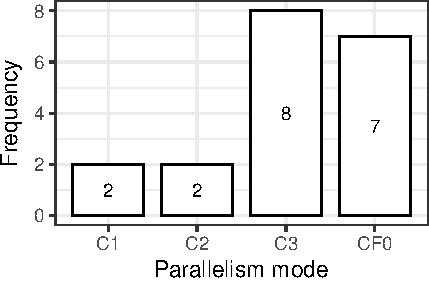
\includegraphics[width=0.32\textwidth]{plots/barplot-modes-dynamic.pdf}
%    \caption{\label{fig:freqmodes-dynamic}\Fix{fix
%    caption}Distribution of parallel modes identified dynamically in a
%    subset of \numProjectsPar{} projects.  A project may have support
%    to more than one parallel mode. Also, a project may run only a
%    subset tests in parallel by default.}
%\end{figure}

%% Recall that some projects can use parallel execution that is only
%% activated when developers pass certain parameters to the build
%% process. For instance, it is possible to create in Maven multiple
%% configurations in the same build file and select dynamically which one
%% should be used.  

\subsubsection{Static checking}
\label{sec:rqC-2}
Given the inherent limitation of dynamic monitoring to find evidence
of parallelism, we also looked for indication of parallelism in build
files\Comment{ in the same sample set of \numMedLong{} projects}.  We
parsed all \emph{pom.xml} files under the project's directory and used
the same approach as in our previous analysis to classify
configurations.  We noticed initially that our approach was unable to
infer the configuration mode for cases where the decision depends on
the input (\eg,
\CodeIn{<parallel>\$\{parallel.type\}</parallel>}). For these
projects, the tester needs to provide additional parameters in the
command line to enable parallelization (\eg, \CodeIn{mvn test
  -Dparallel.type=classesAndMethods}). To handle those case, we
considered all possible values for the parameter (in this case,
\CodeIn{\$\{parallel.type\}}).  It is also important to note that this
approach is not immune to false negatives, which can ocurr when
\emph{pom.xml} files are encapsulated in jar files or downloaded from
the network.  Consequently, this static checking is complementary to
the dynamic checking, previously presented.

Overall, we found, using this methodology, ten projects that use
parallelism.  Compared to the set of projects listed in
Figure~\ref{tab:speedup}, we found two new projects, namely:
\CodeIn{Google Cloud\Comment{ Platform} DataflowJavaSDK} (using
configuration C3) and \CodeIn{Mapstruct} (using configuration
\ForkSeq{}).  Curiously, we also found that project \CodeIn{Jcabi} was
not detected using this methodology.  That happened because this
project loads its \emph{pom.xml} file from a jar file that we did not
check.  Considering the static and dynamic methods together, we found
a total of 11 distinct projects using parallelism, corresponding to
the union of the two subject sets.

\vspace{1ex}
\begin{center}
\fbox{
  \begin{minipage}{8cm}
      \textit{Answering \numRQAdoptionOne{}:}~\emph{Results indicate that test
        suite parallelization is underused.  Overall, only
        \percentParallel{} of costly projects (11 out of \numMedLong)
        use parallelism.}
  \end{minipage}
}
\end{center}
\vspace{1ex}

%False positive can happen because of comments, for instance.  
%To eliminate the cases of false positives and also to categorize 
%true positive cases, we complemented the initial mining step with a 
%manual inspection of files.
%% settings); the second step (inspection) consists in a manual
%% inspection to confirm the presence of parallelism settings in the
%% build file and classify them according to the parallelism level.
%% Figure \Fix{removed} describes the discovery step: we list the paths
%% of all build files and filter only the files that contain any of the

%% Figure~\ref{tab:inspection-table} summarizes our results.
%% \Fix{The first column indicates the group of projects according to
%% their time cost.  The second column indicates the number of build
%% files per group.  The last column indicates the ratio of projects with
%% parallelization settings.  From the \numMedLong{} subjects, we found
%% \pomMedLong{} \pomf{} files.  The \numPomMatched{} configurations are
%% distributed across \numProjectsPar{} projects from our sample.}

%% % \emph{From these results we found that $\sim$51\% of medium and
%% % long-running projects do not use parallel features to run test
%% % suites.}\Mar{please make it consistent with research
%% % question}\Mar{explain this is over(under)-estimated...}
%% \begin{figure}[ht!]
%%     \centering
%%     \resizebox{.48\textwidth}{!}{%
%%     \begin{tabular}{llcl}
%%         \toprule
%%         Group & Subject & \# of modules & Mode\\%
%%         \midrule%
%%         Long   &JenkinsCI Gerrit Trigger Plugin& 1 & \ForkSeq\\%
%%         Medium &Bouncestorage Chaos Http Proxy & 1 & C2\\%
%%         Medium &Javaslang & 1 & C3\\%
%%         Medium &Apache Flink & 1 &\ForkSeq\\%
%%         Medium &Apache Logging Log4J2 & 3 & \ForkSeq{}\\%
%%         Medium &Google Cloud Platform DataflowJavaSDK & 1 & C3\\%
%%         Medium &Hazelcast Jet & 1 & \ForkSeq\\%
%%         Medium &Jankotek MapDB & 1 & C3\\%
%%         Medium &Mapstruct & 1 & \ForkSeq\\%
%%         Medium &Spotify Helios & 3 & \ForkSeq\\%
%%         \bottomrule%
%%     \end{tabular}}
%%     \caption{Subjects with parallelization configurations in build files.}
%%     \label{tab:inspection-table}
%% \end{figure}

%% \begin{figure}[ht!]
%%     \centering
%%     \begin{tabular*}{0.48\textwidth}{@{\extracolsep{\fill}}ccc}
%%         \toprule
%%         \multirow{2}{*}{Group} %1st row, 1st cell
%%             & \multirow{2}{*}{\# \pomf{}}
%% 	    & \# \pomf{} matched\\
%%         % 2nd row - empty cell
%%             & % empty cell
%%             & / total\\%
%%         \midrule%
%% 	Long   & \numPomLong{} & 4 / \numLong{}\\%
%% 	Medium & \numPomMed{} & 6 / \numMed{}\\%
%%         \midrule%
%%         Total % last row, first cell
%%             & \pomMedLong{}
%%             & \numProjectsPar{} / \numMedLong{}\\%
%%         \bottomrule%
%%     \end{tabular*}
%%     \caption{Presence of parallelization settings in build files: the
%%     first column indicates the group of projects according to their
%%     time cost; the second column is the subset of files with parallelization
%%     keywords; the last column indicates the ratio of projects with
%%     parallelism support.}
%%     \label{tab:inspection-table} 
%% \end{figure}
%% \Jbc{rework this... $\rightarrow$} From the \numProjectsPar{} projects
%% identified above, we investigated further the \numPomMatched{}
%% build files with parallel settings.  We analyzed the support and
%% distribution of parallel modes from this subset of projects. To
%% calculate the distribution of parallel modes, we considered only the
%% presence of the mode in at least one of the project settings.  Recall
%% that a build file may contain more than one parallel setting and a
%% project may contain several sub-modules with build files.  In case the
%% value of a parallel option is resolved dynamically (\eg, via
%% command-line argument or system variable) we compute all modes related
%% to the option. For instance, depending on the value, the
%% \CodeIn{parallel} option can be \Seq{} (\CodeIn{none}),
%% \ParClassSeqMeth{} (\CodeIn{classes}), \SeqClassParMeth{},
%% (\CodeIn{methods}), and \ParClassParMeth{} (\CodeIn{all}).
%% Figure~\Fix{fig:freqmodes-static} summarizes our findings.
%% \Fix{Missing conclusion: Fork the most used configuration}
%% \begin{figure}[h!]
%%     \centering
%%     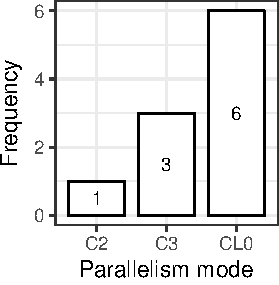
\includegraphics[width=0.32\textwidth]{plots/barplot-modes-static.pdf}
%% 	\caption{\label{fig:freqmodes-static}\Luis{This is wrong, it
%% 	should be \textbf{CF0} instead of \textbf{CL0}}Distribution of parallel modes
%%     identified statically in a subset of \numProjectsPar{} projects.
%%     A project may have support to more than one parallel mode.}
%% \end{figure}


\begin{itemize}
	\item \numRQAdoptionTwo{}. \textbf{\RQAdoptionTwo{}}
\end{itemize}

To answer this research question we surveyed developers involved in a
selection of projects from our benchmark with time-consuming test
suites.  The goal of the survey is to better comprehend developer's
attitude towards the use of parallelism as a mechanism to speedup
regression testing.  We surveyed developers from a total of
\emailsProjects{} projects.  From the initial list of \numMedLong{}
project, we discarded 11 projects that we knew a priori used
parallelization, and \discartedProjects{} projects that we could not find
developer's emails from commit logs.  From this list of projects, we
mined potential participants for our study.  More precisely, we
searched for developer's name and email from the last 20 commits to
the corresponding project repository.  Using this approach, we
identified a total of \emailsSent{} eligible participants.  Finally,
we sent plain-text e-mails, containing the survey, to those developers.  In
total, \emailsAnswered{} developers replied but we discarded
\emailsFalseAnswers{} replies with subjective answers.  Considering
projects covered by the answers, a total of \emailsProjectsAnswered{}
projects (\percEmailsProjectsAnswered{} of the total) were represented
in those replies.  Note that multiple developers on each project
received emails.  We sent the following set of questions to
developers:

\begin{enumerate}
\item How long does it take for tests to run in your environment? Can
  you briefly define your setup?
\item Do you confirm that your regression test suite does *not* run in parallel?
\item\label{questionThree} Select a reason for not using parallelization:
  \begin{enumerate}[label=\alph*)]
  \item I did not know it was possible
  \item I was concerned with concurrency issues
  \item I use a continuous integration server
  \item Some other reason. Please elaborate.
  \end{enumerate}
\end{enumerate}

%% \begin{enumerate}
%% 	\item How long does it take for test to run in your
%%		environment?
%%	\item Can you briefly define your setup?
%%	\item Do you confirm that your project does not run in
%%		parallel?
%%	\item Select a reason for not using paralellization:
%%		\begin{enumarate}
%%			\item I did not know it was possible;
%%			\item I was concerned with concurrency issues;
%%			\item I use a continuous integration server;
%%			\item Some other reason.
%%		\end{enumerate}
%% \end{enumerate}
%% One of the goals of the first questions is to identify potential
%% discrepancies between our experimental environment and the environment
%% of developers.  Overall, we found that \Fix{...}

Considering question 1, we confirmed that execution time was
compatible with the results we reported in Section~\ref{sec:rqA}.
Furthermore, \emailsCI{} of the participants indicated the use of
Continuous Integration (CI) to run tests, with \emailsDistributed{} of
these participants reporting that test suites are modularized and
those modules are tested independetly in CI servers through different
parameters.  Those participants argumented that such practice helps to
reduce time to observe test failures, which is the goal of speeding up
regression testing.  A total of \emailsLocal{} participants answered
that they do run tests in their local machines.  Note, however, that
CI does not preclude low-level parallelization.  For example,
installations of open-source CI tools (\eg{}, Jenkins~\cite{jenkins})
in dedicated servers would benefit from running tests faster through
low-level test suite parallelization.

% \emailsNotDescribed{} developers did not described their environment.

Considering question 2, the answers we collected indicated, to our
surprise, that six of the \emailsProjectsAnswered{} projects execute
tests in parallel.  This mismatch is justified by cases where neither
of our checks (static or dynamic) could detect presence of
parallelism.  A closer look at these projects revealed that one of
them contained a \emph{pom.xml} file encapsulated in a jar file
(similar case as reported in Section~\ref{sec:rqC-2}), in one of the
projects the particpant considered that distributed CI was a form of
parallelism, and in four projects the team preferred to implement
parallelization instead of using existing features from the testing
framework and the build system~---~in two projects the team
implemented concurrency control with custom JUnit test runners and in
two other projects the team implemented concurrency within test
methods.  Note that, considering these four extra cases (ignored two
distributed CI cases), the usage of parallelization increases from
\percentParallel{} to \percentParallelUpdated{}.  We do not consider
this change significant enough to modify our conclusion about
practical adoption of parallelization (\numRQAdoptionOne{}).

%% , one runs a manually created Thread to run some
%% tests, and the other runs in parallel by using Java 8 collection
%% streams, that allows the developers to iterate over a list in
%% parallel.

%% did not confirmed, however,
%% the developers confirmed the need of an extra parameter at the command
%% line to execute in parallel.

Considering question 3, the distribution of answers was as follows.  A
total of \emailsA{} of the \emailsProjectsAnswered{} developers who
answered the survey did not know that parallelism was available in
Maven (option ``a''), \emailsB{} of developers mentioned that they did
not use parallelism concerned with possible concurrency issues (option
``b''), \emailsD{} of developers mentioned that continuous integration
services sufficed to provide timely feedback while running only smoke
\begin{wrapfigure}{r}[0pt]{0pt}%0.525\linewidth
    \centering
    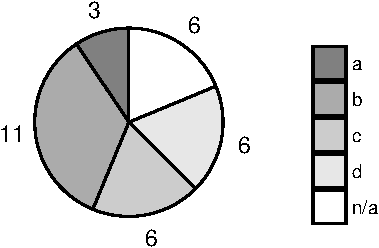
\includegraphics[width=.18\textwidth]{plots/survey.pdf}
    \caption{\label{fig:rq5-answers}Summary of developer's answers to
      survey question~\ref{questionThree}.}
\end{wrapfigure}
tests (\ie{}, short-running tests) locally (option ``c'')\Comment{here
  I want to say that they use it for something like "non-blocking
  testing" while developing in a local machine}, and \emailsD{} of
developers who provided an alternative answer (option ``d'') mentioned
that using parallelism was not worth the effort of preparing the test
suites to take advantage of available processing power.  A total of
\emailsNA{} of participants did not answer the last question of the
survey.  The pie chart in Figure~\ref{fig:rq5-answers} 
summarizes the distribution of answers.

\begin{center}
\fbox{
	\begin{minipage}{8cm}
	  \textit{Answering \numRQAdoptionTwo{}:}~\emph{Results suggest that dealing
       with concurrency issues (\ie{}, the extra work to organize test
       suite to safely explore concurrency) was the principal reason
       for developers not investing in parallelism.  Other reasons
       included availability of continuous integration services and
       unfamiliarity with the technology.}
	\end{minipage}
}
\end{center}

\subsection{Speedups}
\label{sec:rqD}

\begin{itemize}
    \item \numRQSpeedupOne{}. \textbf{\RQSpeedupOne}
\end{itemize}

To answer \numRQSpeedupOne{}, we considered the \numProjectsPar{}
subjects from our benchmark that use parallelization \emph{by default}
(see Figure~\ref{tab:freqmodes-dynamic}).  We compared running times
with parallelization~---~configured by project owners~---~and without
parallelization.

%% In those projects, parallelization is active without
%% passing any extra parameters.  Section~\ref{sec:rqC-1} describes in
%% detail the methodology we used to find these subjects.
%and
%Section~\ref{seq:rq6-tradeoffs}, we verified that both
%% executions produce the same outcome to eliminate noise from failing
%% tests.  To compute the speedup, we divide the time obtained in the
%% sequential execution by the time obtained from the default execution.
%% For instance, if a project runs the tests sequentially in $10m$ and
%% the same execution runs in $5m$ with parallelization enabled (default
%% execution), the speedup is two.

Figure~\ref{tab:speedup} summarizes results.  Lines are sorted by
project names.  Columns ``\emph{Group}'' and
``\emph{Name}'' indicate, respectively, the group and the name of the
subject.  Column ``$T_s$'' shows sequential execution time and column
``$T_p$'' shows parallel execution time. Column ``$T_s/T_p$'' shows
speedup or slowdown.  As usual, a ratio above 1x denotes speedup
and a ratio below 1x denotes slowdown.

\begin{figure}[h!]
\centering
\resizebox{.41\textwidth}{!}{%
  \scriptsize
\begin{tabular}{llrrr}
\toprule
\emph{Group} & \emph{Subject} & \multicolumn{1}{c}{$T_s$} & \multicolumn{1}{c}{$T_p$} & $T_s/T_p$ \\%
\midrule%
Medium & \Comment{BounceStorage }Chaos\Comment{ HTTP Proxy} & 1.51m & 1.47m & 
    \cellcolor{lightgray}1.01x\\%
Medium &\Comment{ Apache }Flink& 11.79m & 2.57m & 4.59x\\%
Long &\Comment{ Jenkins CI }Gerrit\Comment{ Plugin} & 51.19m & 40.31m &  1.26x\\%
Medium &\Comment{ Spotify }Helios& 4.46m & 1.63m & 2.73x\\%  
Medium &Javaslang& 2.18m & 1.82m & 1.19x\\%
Medium &Jcabi\Comment{ GitHub} & 2.76m & 0.30m &
    \cellcolor{lightgray}9.2x\\%
Medium &\Comment{ Hazelcast }Jet& 8.26m & 3.67m & 2.25x\\%
Long &\Comment{ Apache }Log4J2& 8.24m & 8.21m & \cellcolor{lightgray}1.00x\\%
Long &\Comment{ Jankotek }MapDB& 10.06m & 8.58m & 1.17x\\%
\midrule
\textbf{average} &  &  &  & \avgSpeedup{}x\\
\bottomrule%
\end{tabular}}
\caption{\label{tab:speedup}Speedup (or slowdown) of parallel
  execution ($T_p$) over sequential execution ($T_s$).  Default
  parallel configuration of Maven is used.  Highest slowdown/speedup
  appears in gray color.}
\end{figure}

Results indicate that, on average, parallel execution was
\avgSpeedup{} times faster compared to sequential execution.  Three
cases worth special attention: \CodeIn{Chaos}, \CodeIn{Jcabi} and
\CodeIn{Log4J2}.  No significant speedup was observed in
\CodeIn{Chaos}, a project with only three test classes, of which one
monopolizes the bulk of test execution time.  This project uses
configuration \ParClassSeqMeth{}, which runs test classes in parallel
and test methods, declared in each class, sequentially.  Consequently,
speedup cannot be obtained as the cost of the single expensive test
class cannot be broken down with the selected configuration.  Although
project \CodeIn{Jcabi} also uses configuration \ParClassSeqMeth{},
results obtained are very different compared to \CodeIn{Chaos}.  The
speedup observed in \CodeIn{Jcabi} was the highest amongst all
projects.  This project contains test classes with a small number of
test methods and several methods in those classes are time-consuming.
As result, the CPUs available for testing are kept occupied for the
most part during test execution.  Finally, we note that parallel
execution in \CodeIn{Log4J2} was innefective.  We found that Maven
invokes several test modules in this project but the test modules that
dominate execution time run sequentially by default.

%% The third, runs parallel configuration in
%% \Fix{80\%} of the project modules, however, the test time is dominated
%% by one of the sequentially running modules.  \Luis{$\leftarrow$ rework
%%   this} \Fix{falar sobre o resultado geral dos speedups - elaborar
%%   menor e maior speedup... acho que so vale a pena discutir quando
%%   tiver conviccao dos 2 casos}

\begin{center}
\fbox{
  \begin{minipage}{8cm}
    \textit{Answering \numRQSpeedupOne{}:}~\emph{Considering the
      machine setup we used, the average speedup observed with default
      configurations of parallelization was \avgSpeedup{}x.}
  \end{minipage}
}
\end{center}

\begin{itemize}
    \item \numRQSpeedupTwo{}. \textbf{\RQSpeedupTwo}
\end{itemize}

\newcommand{\subjectScalability}{MapDB}

This experiment evaluates the impact of making available to the build
system a growing number of CPUs for testing.  For that reason, we used
a machine with more cores compared to the one described in
Section~\ref{sec:setup}.  We used a Xeon E5-2660v2 (2.20GHz) Intel
processor machine with 80 virtual CPUs (40 cores with two native
threads each) and 256GB of memory, running Ubuntu 14.04 LTS Trusty
Tarr (64-bit version). This experiment uses configuration \ForkSeq{}
\begin{wrapfigure}{r}[0pt]{0pt}%0.525\linewidth
    \centering
    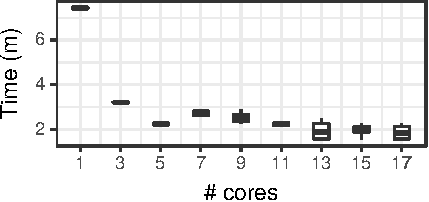
\includegraphics[width=.2\textwidth]{R/scalability/scalability.pdf}
    \caption{\label{fig:scalability}Scalability.}
\end{wrapfigure}
as the goal is to evaluate the impact on runtime of spawning a growing number of
JVMs in different CPUs.  Furthremore, we selected subject
\subjectScalability{} as it represents the case of a long-running test
suite (see Figure~\ref{tab:speedup}) with test cases distributed
across many test classes (194 test classes for \subjectScalability{}).
Note that a test class is the smallest unit that can be used to spawn
a test job on a JVM and that we have no control over which test
classes will be assigned to which JVM that the build system forks.

Figure~\ref{fig:scalability} shows the reduction of running times as
more CPUs contribute to the execution.  \Fix{elaborate...}

\begin{center}
\fbox{
  \begin{minipage}{8cm}
    \textit{Answering \numRQSpeedupTwo{}:}~\emph{...}
  \end{minipage}
}
\end{center}

\subsection{Issues}
\label{sec:rq6-tradeoffs}

This dimension assesses the impact of using distinct parallel
configurations on test flakiness (negative impact) and speedup
(positive impact).  Furthermore, note that Section~\ref{sec:rqD}
evaluated speedup in isolation, focused on projects configured to use
parallelism by default.

\begin{itemize}
    \item \numRQIssuesOne{}. \textbf{\RQIssuesOne{}}
\end{itemize}


%% The intuition is that efficiency and flakiness are inversely
%% proportional in some cases: if too many tests depends on the state of
%% a single external resource, several tests are likely to fail as the
%% degree of concurrency increases by exploiting maximum CPU usage.

%% Table header macros
% $\Uparrow_\text{speed}$
\newcommand{\subcolA}{$\text{speedup}$}
\newcommand{\subcolB}{$\%_\text{fail}$}
\newcommand{\colheader}[1]{\multicolumn{2}{c}{\emph{#1}}}
\newcommand{\blankentry}{\entry{-}{-}}
\newcommand{\subcol}{\subcolA{} & \subcolB{}}
\newcommand{\entry}[2]{#1 & #2}

\begin{figure*}[t]  
\centering
\small
\setlength{\tabcolsep}{3pt}
\begin{tabular}{l|rr|rr|rr|rr|rr|rr}
\toprule
\multirow{2}{*}{\emph{Subject (module)}} & \multicolumn{2}{c|}{\emph{\Seq}} &
    \colheader{\SeqClassParMeth} & \colheader{\ParClassSeqMeth} &
    \colheader{\ParClassParMeth} & \colheader{\ForkSeq} &
    \colheader{\ForkParMeth} \\ %\cline{2-12}
    & $T$ & $\mathit{N}$ & \subcol{} & \subcol{} & \subcol{} & \subcol{}
    & \subcol{}\\%
\midrule%
AWS SDK Java (\CodeIn{core})  & \entry{3.7m}{847}  & \entry{1.95x}{2.24\%} & \entry{2.47x}{2.77\%} & \entry{3.70x}{4.01\%} & \entry{}{} & \entry{}{}\\%

Facebook Linkbench    & \entry{4.3m}{98}  & \entry{1.00x}{0\%} & \entry{1.65x}{1.02\%} & \entry{1.59x}{1.02\%} & \entry{}{} & \entry{}{}\\%

GoogleCloud Dataflow Java (\CodeIn{sdk}) & \entry{1.6m}{3,345}  & \entry{1.23x}{1.67\%} & \entry{2.67x}{1.05\%} & \entry{0.80x}{5.35\%} & \entry{}{} & \entry{}{}\\%

Javaslang (\CodeIn{core})     & \entry{1.1m}{17,513}  & \entry{1.38x}{0\%} & \entry{1.83x}{0\%} & \entry{1.38x}{0\%} & \entry{}{} & \entry{}{}\\ 
JCabi Github                  & \entry{2.6m}{634} & \entry{2.10x}{0\%} & \entry{17.70x}{0\%} & \entry{28.80x}{0\%} & \entry{}{} & \entry{}{} \\
JCTools (\CodeIn{core})       & \entry{3.6m}{690}  & \entry{4.50x}{0\%} & \entry{3.60x}{0\%} & \entry{18.00x}{0\%} & \entry{}{} & \entry{}{}\\%
MapDB  & \entry{8.2m}{5,324}  & \entry{1.52x}{0\%} & \entry{2.73x}{0\%} & \entry{4.82x}{0.05\%}   & \entry{}{} & \entry{}{}\\%
Moquette                      & \entry{3.7m}{169} & \entry{4.62x}{65.64\%} & \entry{3.36x}{32.92\%} & \entry{12.33x}{77.78\%} & \entry{}{} & \entry{}{} \\
RipMe                         & \entry{1.1m}{54}  & \entry{0.94x}{0\%} & \entry{1.63x}{0\%} & \entry{1.63x}{0\%} & \entry{1.37x}{0\%} & \entry{1.42x}{0\%}\\
Stripe Java     & \entry{4.3m}{302}  & \entry{4.78x}{6.31\%} & \entry{3.31x}{7.31\%} & \entry{21.50x}{14.95\%} & \entry{}{} & \entry{}{}\\%





\midrule

\textbf{Average}   & \entry{-}{-} & \entry{-}{-} & \entry{-}{-} & \entry{-}{-}
& \entry{-}{-} & \entry{-}{-} \\%


%%  & \entry{x.xm}{0}  & \entry{}{\%} & \entry{}{\%} & \entry{}{\%} & \entry{}{} & \entry{}{}\\%
%%OpenMRS Core (\CodeIn{api})  & \entry{15.4m}{3436} & \blankentry{}        & \blankentry{}        & \blankentry{} & \entry{1.5x}{0\%} & \entry{1.7x}{0}\\%
%%Apache Flume (\CodeIn{core}) &  \entry{7.7m}{392}  & \blankentry{}        & \blankentry{}        & \blankentry{}       & \entry{0.9x}{0\%} & \blankentry{} \\%
%%Facebook Archive Linkbench   &  \entry{4.5m}{98}   & \entry{1.0x}{0.2\%}  & \entry{1.6x}{1.2\%}       & \entry{1.0x}{0\%}  & \entry{1.7x}{0.5\%}  & \entry{1.7x}{0.2\%}\\%
%%AWS SDK Java (\CodeIn{core}) &  \entry{3.8m}{847}  & \multicolumn{6}{c}{\Fix{requires investigation}} & \entry{2.2x}{0.1\%} & \entry{3.2x}{2.0\%}\\%

%% OpenMRS Core (\CodeIn{api})  & \entry{15.4m}{3436} & \blankentry{}        & \blankentry{}        & \blankentry{} & \entry{1.5x}{0\%} & \entry{1.7x}{0}\\%
%% Jankotek MapDB               &  \entry{9.9m}{5218} & \multicolumn{6}{c}{\cellcolor{lightgray}\emph{JVM Crash}} & \entry{1.5x}{0\%} & \entry{1.7x}{0\%}\\%
%% Apache Flume (\CodeIn{core}) &  \entry{7.7m}{392}  & \blankentry{}        & \blankentry{}        & \blankentry{}       & \entry{0.9x}{0\%} & \blankentry{} \\%
%% Apache Giraph (\CodeIn{core})&  \entry{7.2m}{236}  & \entry{2.1x}{5.1\%}  & \colheader{\cellcolor{lightgray}timeout}   & \entry{1.0x}{0\%} & \entry{1.0x}{0}\% & \colheader{\cellcolor{lightgray}JVM Crash}\\%
%% Facebook Archive Linkbench   &  \entry{4.5m}{98}   & \entry{1.0x}{0.2\%}  & \entry{1.6x}{1.2\%}       & \entry{1.0x}{0\%}  & \entry{1.7x}{0.5\%}  & \entry{1.7x}{0.2\%}\\%
%% Stripe Java                  &  \entry{4.2m}{302}  & \entry{4.2x}{5.2\%}  & \entry{3.5x}{5.7\%}       & \entry{4.2x}{6.3\%} & \entry{1.0x}{0.3\%} & \entry{4.2x}{5.7\%}\\%
%% AWS SDK Java (\CodeIn{core}) &  \entry{3.8m}{847}  & \multicolumn{6}{c}{\Fix{requires investigation}} & \entry{2.2x}{0.1\%} & \entry{3.2x}{2.0\%}\\%

%% Jenkins CI Github            & \entry{Xm}{Z}       & \entry{x}{\%}          & \entry{x}{\%} & \entry{x}{\%} & \entry{x}{\%} & \entry{x}{\%}\\%
%% Jenkins CI Docker Workflow   & \entry{Xm}{Z}       & \entry{x}{\%}          & \entry{x}{\%} & \entry{x}{\%} & \entry{x}{\%} & \entry{x}{\%}\\%
%% Hazelcast                    & \entry{Xm}{Z}       & \entry{x}{\%}          & \entry{x}{\%} & \entry{x}{\%} & \entry{x}{\%} & \entry{x}{\%}\\%

\bottomrule%
\end{tabular}
\caption{Speedup versus Flakiness (\subcolB). Configuration
  \emph{\Seq{}} denotes the comparison baseline, which runs tests
  sequentially.  Columns $T$ and $N$ indicate time and number of
  tests, respectively.  Other columns show speedup and percentage of
  failing tests in different configurations, compared to
  \emph{\Seq{}}.\Mar{Can you please add name of module for all subjects?}}
\label{tab:rq6-table}
\end{figure*}

To answer this research question, we conducted an experiment involving
the six parallel configurations from Section~\ref{sec:modes}  and the
top 10 long-running test modules from our sample set. The rationale
for this selection criteria was to maximize the chances of observing
speedup and flakiness, assuming that long-running tests also have many
tests. Indeed, we confirmed that test suites in these projects contain
at least 236 tests ($1,662.7$ in average). Also, we preferred to compare the
effect of a configuration over a single test module for projects with
multiple test modules.  Recall that large projects may contain several
test modules, and these modules may contain distinct characteristics
that could favor one configuration and not others; therefore, it would
be necessary to check each module individually for a fair comparison.
We are interested in understanding how efficiency (\ie, testing cost)
and flakiness (\ie, failing tests) are affected when we run a test
suite with different parallel configurations.  Recall that increased
resource contention obtained with parallelism can lead to concurrency
issues such as data races.  Flakiness and speedup are contradictory
forces that drive configuration selection.  We used as a \emph{control
group} (\ie, baseline) the sequential execution of each subject's
tests. Notice that for measuring flakiness, we have to consider only
tests that failed due to the concurrency in the parallel execution.
For that reason, we re-executed the tests in sequence ten times and
carefully verified that there are only passing tests in our baseline.
We considered ten as the number of re-executions based on the approach
used by Google reported in a previous work on test
flakiness~\cite{luo-etal-fse2014}.  To obtain parallel configurations,
we implemented a script that takes a subject and a configuration (\eg,
\ForkSeq{}) as inputs, and the script outputs the modified version of
the subject with the desired configuration. The workflow consists in
copying the project directory to a new directory, finding all existing
build files (\ie, \pomf{} files), and modifying all existing Maven
Surefire configurations with new values for the parameters
\CodeIn{parallel}, \CodeIn{forkCount}, and \CodeIn{threadCount} using
an XPath~\cite{xpath} library to manipulate XML documents. For
configurations with forked JVMs enabled (\ie, \ForkSeq{} and
\ForkParMeth{}), we changed the \CodeIn{forkCount} with the value
\CodeIn{1C} (\ie, one JVM per core).  To adjust the pool of threads
for parallelism within a JVM, we changed the parameter
\CodeIn{threadCount} with \Jbc{should we consider 2 as it is the
number of native threads per core OR 6 as it represents 3 Cores * 2
native threads?}.  To run the subjects and their respective variations
(\ie, the modified versions according to the parallelism
configuration), we used a similar approach as described in


Figure~\ref{fig:mvn-execution} except that we added a timeout of one
hour to run the tests. We used the \CodeIn{timeout}
command~\cite{timeout-cmd} to monitor the execution, and we configured
the command to dispatch a \emph{kill} signal if the test execution
exceeds the time limit. We imposed this time constraint to avoid
hanging indefinitely the experiment execution due to some thread
contention that may occur (\eg, deadlock). Finally, we saved each
execution log and XML test reports generated by Maven to collect the
execution time, the number of failing tests, and for reference to
analyze and diagnose outliers in our results. For efficiency, we
reported the speedup (\ie, $\Uparrow_\text{speed} = T_{\text{s}} /
T_{\text{p}}$) in average, and for flakiness, we reported the rate of
failing tests (\ie, $\mathit{\%_\text{fail} = failures / tests}$) in
average.  Figure~\ref{tab:rq6-table} summarizes the obtained results
ordered by the time cost (\ie, $T_\text{cost}$). \Fix{Remember to
explain efficiency cutoff, JVM crashes and timeout}

\Jbc{Lembrar que investigar o slowdown de Dataflow... os logs indicam que varios
dos testes que quebraram tentavam fazer uma autenticacao em algum servico.
Possivelmente o slowdown se deve ao tempo de resposta do servico quando
a autentiticao falha}

%% \begin{figure}[h!]
%% \centering
%% \resizebox{.48\textwidth}{!}{%
%% \begin{tabular}{lcrrrrr}
%% \toprule
%% \emph{Subject} & \emph{\# of tests} & \emph{\SeqClassParMeth{}} & \emph{\ParClassSeqMeth{}} & \emph{\ParClassParMeth{}} & \emph{\ForkSeq{}} & \emph{\ForkParMeth{}}\\%
%% \midrule%
%% Linkedin Pinot & 356 & - & - & - & - & -\\%
%% %% Jenkins CI Github Plugin & - & - & - & - & 0\% & -\\%
%% %% Kite SDK & - & - & - & - & - & -\\%
%% %% \Fix{!?} Apache Giraph & 327 & - & - & - & - & -\\%
%% %% OpenMRS Core & - & - & - & - & - & -\\%
%% %% Jenkins CI Docker Workflow Plugin & - & - & - & - & 0\% & -\\%
%% %% \Fix{Flaky} Apache Eagle & - & - & - & - & - & -\\%
%% %%Geotools & 7701 & - & - & - & - & -\\%
%% %%Kuromoji & 672 & - & - & - & - & -\\%
%% %%Atomix & 99 & - & - & - & - & -\\%
%% %%\Fix{Snazy OHC} & - & - & - & - & - & -\\%
%% %%\Fix{RoaringBitmap} & - & - & - & - & - & -\\%
%% \bottomrule%
%% \end{tabular}}
%% \caption{\Fix{Tabela de flakiness}}
%% \label{tab:rq6-flaky}
%% \end{figure}

\Fix{Elaborate results from efficiency}

\Fix{Elaborate results from flakiness}

\Fix{highlight special cases}

\Fix{Draw conclusions}

\begin{center}
\fbox{
\begin{minipage}{8cm}
\textit{Answering \numRQIssuesOne{}:~\emph{\Jbc{summarize findings...}}}
\end{minipage}
}
\end{center}

%%  LocalWords:  RQ occurence parallelization Tradeoffs API readme th
%%  LocalWords:  mvn clearcut escapeinside xleftmargin untestable LTS
%%  LocalWords:  framexleftmargin CPUs Tahr sysstat gh Vagrantfile
%%  LocalWords:  javadoc isolcpus JUnit's JUnitCore Gligoric boxplots
%%  LocalWords:  outliers apache uber chaperone facebookarchive
%%  LocalWords:  linkbench priori

\chapter{Discussion}

This paper reports our finding on a study to evaluate impact and usage
of test suite parallelization, enabled by modern build systems and
testing frameworks.  This study is important given the importance to
speedup testing.  Note that test suite parallelization is
complementary to alternative approach to speedup testing
(see~Section~\ref{sec:related}).  The observations we made in this
study trigger multiple actions:

\begin{itemize}
\item \emph{Incentivize forking.}~Forked JVMs manifest low rates of
  test flakiness.  For instance, in \emph{\ForkSeq{}}, only 4 of 10
  projects manifest flakiness and, excluding the extreme case of
  \CodeIn{Moquette}, projects manifest flaky tests in low rates 0.23\%
  to 1.70\%.  Developers of projects with long-running test suites
  should consider using that feature, which is available in modern
  build systems today (\eg{}, Maven).
\item \emph{Break test dependencies.}~Non-forked JVMs can achieve
  impressive speedups at the expense of sometimes impressive rates of
  flakiness.  Breaking test dependencies to avoid flakiness and take
  full advantage of those options is advised for developers with
  greater interest in efficiency.
\item \emph{Refactor tests for load balancing.}~Forked JVMs scales
  better with the number of cores when the test workload is balanced
  across testing classes.  To balance the workload, automated
  user-oblivious refactoring can help in scenarios where developers
  are not willing to change test code but have access to machines with
  a high number of cores.
\item \emph{Improve debugging for build systems.}~While preparing our
  experiments, we found scenarios\Comment{, related to test
    parallelization,} where Maven's executions did not reflect
  corresponding JUnit's executions. \Comment{(Docker reproduction scripts
  available.)} Those issues can hinder developers from using parallel
  testing. Better debugging infrastructure is important.
\end{itemize}

This study brings to light the benefits and burdens of test suite
parallelization to improve test efficiency. It provides
recommendations to practitioners and developers of new techniques and
tools aiming to speed up test execution with parallelization.


%%  LocalWords:  parallelization Incentivize JVMs Moquette Refactor
%%  LocalWords:  refactoring JUnit's

\section{Threats to Validity}

The main threats to validity of this study are the following.

\textit{External Validity:} Generalization of our findings is limited
to our selection of subjects, testing framework, and build system.  To
mitigate that issue, we selected subjects according to an objective
criteria, described in Section~\ref{sec:subjects}.  It remains to
evaluate the extent to which our observations would change when using
different testing frameworks and build systems.
Also, some of the selected subjects contain failing tests. Test
failures may reduce the testing time due to early termination
or even inflate the time (\eg, test waiting indefinitely for
an unavailable resources).
To mitigate this threat, we eliminated subjects with flaky tests and
filtered projects with at least 90\% of the tests passing.
Only 17\% of our subjects have failing tests.
We carefully inspected our rawdata to identify and ignore these
failures with JUnit's \CodeIn{@Ignore} annotation.

\textit{Internal Validity:} Our results could be influenced by
unintentional mistakes made by humans who interpreted survey data and
implemented scripts and code to collect and analyze the data.
For example, we developed JUnit runners to reproduce Maven's parallel
configurations and implemented several scripts to automate our
experiments (\eg, run tests and detect parallelism enabled by default
in the subjects).
All those tasks could bias our results.
To mitigate those threats, the first two authors of this paper
validated/inspected each other to increase chances of capturing
unintentional mistakes.

\textit{Construct Validity:} We considered a number of metrics in this
study that could influence some of our interpretations.  For example,
we measured number of test cases per suite, distribution of test costs
in a suite, time to run a suite, etc.  In principle, these metrics may
not reflect the main problems associated with test
efficiency.

%%  LocalWords:  QA dockerfile StackOverflow

\section{Related Work}
\label{sec:related}
We discuss most related work in the following.
%% Researchers and practitioners have been shedding light to the demand
%% of techniques for optimizing test execution.

%% For instance, a recent paper from the automotive industry reported
%% that test suites can take days to run~\cite{artl-etal-icst2015}.
%% There are different aspects to consider when dealing with the
%% challenge of reducing test cost.

%ekstazi-web,
Regression testing research has focused mostly on test suite
minimization, prioritization, reduction, and
selection~\cite{yoo-harman-stvr2012,soetens-etal-2016}.  Most of these
techniques are unsoud (\ie{}, they do not guarantee that
fault-revealing tests will be considered for testing).  The test
selection technique
Ekstazi~\cite{gligoric-etal-issta2015,celik-etal-fse2017} is an
example of a sound regression testing technique. It conservatively
computes which tests have been impacted by file changes.  A test is
discarded for execution if it does not depend on any changed file
dynamically reachable from execution.\Comment{ Curiously Ekstazi's
  evaluation discovered subjects with parallelism enabled by
  default.}\Comment{ \c{C}elik~\etal{}~\cite{} recently extended
  Ekstazi to track files accessed outside JVM boundaries.} Important
to note that regression testing techniques, including test selection,
is complementary to test suite parallelization.

%\Luis{maybe we should create another division for test acceleration}

ElectricTest~\cite{bell-etal-esecfse2015} is a tool for efficiently
detecting data dependencies across test cases.  Dependency tracking is
important as to avoid test flakiness when parallelizing test
suites. ElectricTest observes reads and writes on global resources
made by tests to identify these dependencies at low cost. We remain to
investigate the impact of ElectricTest to reduce flakiness in
unrestricted test suite parallelization.

%% \textit{Usage of massively parallel hardware:}
%\textit{Hardware level massive parallelization:}

The use of the Single Instruction Multiple Data (SIMD) design has been
previoulsy explored in research to accelerate test
execution~\cite{damorim-etal-issta2007,damorim-etal-tse2008,kim-etal-issre2012,nguyen-etal-icse2014,rajan-etal-ase2014,sen-etal-fse2015,yaneva-etal-issta2017}. The
SIMD architecture, as implemented in modern GPUs, for instance, allows
the execution of a given instruction simultaneously against multiple
data.  For that reason, in principle, one test could be ran
simulteneously against multiple inputs provided that multiple test
inputs exist associated to that one test.  Recent
work~\cite{rajan-etal-ase2014,yaneva-etal-issta2017} explored that
idea to speedup test execution of embedded software using graphic
cards. Although benchmarks indicate superior performance compared to
traditional multicore CPUs, the use of the technology in broader
settings is limited. For example, execution of more general programs
can violate the SIMD's lock-step assumption on the control-flow of
threads.  This violation would affect negatively performance.
Furthermore, handling complex data is challenging in
SIMD~\cite{damorim-etal-issta2007,damorim-etal-tse2008}.  The approach
is promising when multiple input vectors exist for each test and the
testing code heavily manipulates scalar data types.  The datasets used
in those papers satisfied those constraints.


%% existing GPU programming-models (\eg{}, CUDA~\cite{cuda}, and
%% OpenCL~\cite{opencl}) are compatible only with a subset of the C/C++
%% language.
%% Recent work proposed a compiler-assisted approach to make programs
%% compatible with the relying programming-model used by
%% GPUs to parallelize tests~\cite{}.
%% \Jbc{...Justify they are out of scope for our subjects...}.

\Mar{can you complete this AND add text on high-level paralellism?}

\textit{Continuous integration services:}
Recent work showed us that Continuous Integration Services are widely
used and improve the productivity~\Fix{ref ref ref}. 

%% \Jbc{Missing work about testing in the cloud and Jon Bell}

\Comment{
\Fix{Please:
  (i) consider categorizing related work in sections  
  (ii) list papers that need to be discussed
  (iii) discuss papers that use multi-execution (SIMD cpus like GPUs)
  to speedup testing
  }
}
\Comment{
Similar approach to regression test selection has been recently
applied in the context of the GCC~\cite{gcc} configurable
system~\cite{souto-damorim-jss}.
O Trabalho de Hilton et al~\cite{hilton-etal-ase2016}, embora tenha
como objetivo entender o uso de CI, mostra que existe uma demanda em
acelerar o build e execucao de testes em servidores de integracao
    continua
}

\section{Conclusions}

Testing is expensive.  Despite all advances in regression testing
research, dealing with high testing costs remains an important problem
in Software Engineering.  This paper reports our findings on the usage
and impact of test execution parallelization in open-source projects.
Multicore CPUs, as well as testing frameworks and build systems to
capitalize on them, are widely available today.  Despite some
resistance observed from practicioners, our results suggest that
parallelization can be done in many cases without sacrificing
reliability and more research needs to be done to improve automation
(\eg{}, breaking test dependencies and refactoring test suites) as to
safely optimize parallel execution.  The artifacts we produced as
result of this study are available from the following web
page \webpage{}.


%% Overall, this study brings to light the benefits and burdens of test
%% suite parallelization to improve test efficiency. It provides
%% recommendations to practicioners and developers of new techniques and
%% tools aiming to speed up test execution with parallelization.

%% Considering a set of \numSubjs{} popular Java projects we analyzed, we
%% found that \percentMedLongRunning{} of the projects contain costly
%% test suites but parallelization features still seem underutilized in
%% practice~---~only \percentParallelUpdated{} of costly projects use
%% parallelization.  The main reported reason for adoption resistance was
%% the concern to deal with concurrency issues.  Results suggest that, on
%% average, developers prefer high predictability than high performance
%% in running tests.







% if have a single appendix:
%\appendix[Proof of the Zonklar Equations]
% or
%\appendix  % for no appendix heading
% do not use \section anymore after \appendix, only \section*
% is possibly needed

% use appendices with more than one appendix
% then use \section to start each appendix
% you must declare a \section before using any
% \subsection or using \label (\appendices by itself
% starts a section numbered zero.)

% \appendices
% \section{Proof of the First Zonklar Equation}
% Appendix one text goes here.
% 
% % you can choose not to have a title for an appendix
% % if you want by leaving the argument blank
% \section{}
% Appendix two text goes here.


% use section* for acknowledgment
\ifCLASSOPTIONcompsoc
  % The Computer Society usually uses the plural form
  \section*{Acknowledgments}
\else
  % regular IEEE prefers the singular form
  \section*{Acknowledgment}
\fi


Jean(derson) and Luis are supported by FACEPE scholarphips
IBPG-0632-1.03/15 and IBPG-1175-1.03/16, respectively.  This work was
partially supported by CNPq grants 457756/2014-4 and 203981/2014-6.


% Can use something like this to put references on a page
% by themselves when using endfloat and the captionsoff option.
\ifCLASSOPTIONcaptionsoff
  \newpage
\fi



% trigger a \newpage just before the given reference
% number - used to balance the columns on the last page
% adjust value as needed - may need to be readjusted if
% the document is modified later
%\IEEEtriggeratref{8}
% The "triggered" command can be changed if desired:
%\IEEEtriggercmd{\enlargethispage{-5in}}

% references section

% can use a bibliography generated by BibTeX as a .bbl file
% BibTeX documentation can be easily obtained at:
% http://mirror.ctan.org/biblio/bibtex/contrib/doc/
% The IEEEtran BibTeX style support page is at:
% http://www.michaelshell.org/tex/ieeetran/bibtex/
%\bibliographystyle{IEEEtran}
% argument is your BibTeX string definitions and bibliography database(s)
%\bibliography{IEEEabrv,../bib/paper}
%
% <OR> manually copy in the resultant .bbl file
% set second argument of \begin to the number of references
% (used to reserve space for the reference number labels box)
\bibliographystyle{IEEEtran}
\bibliography{tmp}

% biography section
% 
% If you have an EPS/PDF photo (graphicx package needed) extra braces are
% needed around the contents of the optional argument to biography to prevent
% the LaTeX parser from getting confused when it sees the complicated
% \includegraphics command within an optional argument. (You could create
% your own custom macro containing the \includegraphics command to make things
% simpler here.)
%\begin{IEEEbiography}[{\includegraphics[width=1in,height=1.25in,clip,keepaspectratio]{mshell}}]{Michael Shell}
% or if you just want to reserve a space for a photo:

\begin{IEEEbiography}{Michael Shell}
Biography text here.
\end{IEEEbiography}

% if you will not have a photo at all:
\begin{IEEEbiographynophoto}{John Doe}
Biography text here.
\end{IEEEbiographynophoto}

% insert where needed to balance the two columns on the last page with
% biographies
%\newpage

\begin{IEEEbiographynophoto}{Jane Doe}
Biography text here.
\end{IEEEbiographynophoto}

% You can push biographies down or up by placing
% a \vfill before or after them. The appropriate
% use of \vfill depends on what kind of text is
% on the last page and whether or not the columns
% are being equalized.

%\vfill

% Can be used to pull up biographies so that the bottom of the last one
% is flush with the other column.
%\enlargethispage{-5in}



% that's all folks
\end{document}


